% !TeX root = main.tex
\documentclass{article}
\usepackage[utf8]{inputenc}
\usepackage[T1]{fontenc} % Meglio per i caratteri accentati in locale
\usepackage[italian]{babel} % Per sillabazione e titoli automatici (es. "Indice")

\usepackage{array}
\usepackage{tabularx}
\usepackage{booktabs}
\usepackage{graphicx}
\usepackage{hyperref}
\usepackage{float}
\usepackage{svg}
\usepackage{fancyhdr}
\usepackage{geometry}
\geometry{a4paper, margin=1in}
\usepackage{pdfpages}
\usepackage[most]{tcolorbox}
\usepackage{tabularx}
\usepackage{booktabs}
\usepackage{pgfplots}
\usepgfplotslibrary{polar}
\pgfplotsset{compat=1.18}

% --- GESTIONE COLORI (Tutti qui, senza duplicati) ---
\usepackage[table, svgnames]{xcolor} 
\definecolor{codegreen}{rgb}{0,0.6,0}
\definecolor{codegray}{rgb}{0.5,0.5,0.5}
\definecolor{codepurple}{rgb}{0.58,0,0.82}
\definecolor{backcolour}{rgb}{0.97,0.97,0.98}
\definecolor{DarkBlue}{HTML}{356698}
\definecolor{highlight}{HTML}{0072B2} % Definizione mancante aggiunta qui
% Definizione dei colori della palette
\definecolor{DeepNavy}{HTML}{173857}
\definecolor{SteelBlue}{HTML}{4D7396}
\definecolor{DeepEarth}{HTML}{573E17}
\definecolor{SandGold}{HTML}{AC9166}
\definecolor{WarmCream}{HTML}{FFF3DF}
\definecolor{AccentOrange}{HTML}{F39C12}

% --- CONFIGURAZIONE LISTINGS ---
\usepackage{listings}
\lstdefinelanguage{JavaScript}{
  keywords={break, case, catch, continue, debugger, default, delete, do, else, false, finally, for, function, if, in, instanceof, new, null, return, switch, this, throw, true, try, typeof, var, void, while, with, const, let, async, await, export, default, import, from, expect, it, describe, toBe, toBeTrue, toThrowError},
  morecomment=[l]{//},
  morecomment=[s]{/*}{*/},
  morestring=[b]',
  morestring=[b]",
  morestring=[b]`
}

\lstdefinestyle{mystyle}{
    backgroundcolor=\color{backcolour},   
    commentstyle=\color{codegreen},
    keywordstyle=\color{DarkBlue}\bfseries,
    numberstyle=\tiny\color{codegray},
    stringstyle=\color{codepurple},
    basicstyle=\ttfamily\footnotesize,
    breaklines=true,                 
    captionpos=b,                    
    numbers=left,                    
    numbersep=5pt,                  
    tabsize=2,
    language=JavaScript,
    showstringspaces=false
}
\lstset{style=mystyle}

% --- INTESTAZIONI ---
\pagestyle{fancy}
\fancyhf{}
\renewcommand{\headrulewidth}{0pt}
\fancyfoot[C]{%
    \textcolor{DarkBlue}{\rule{\textwidth}{1.5pt}} \\
    \textcolor{DarkBlue}{\textbf{\small Dieti Estates -- \textbf{a.a. 2024/2025}}}%
    \hfill%
    \textcolor{black}{\textbf{\textsf{\fboxsep=6pt{\thepage}}}}
}

\renewcommand{\contentsname}{Indice} % to change the title of table of contents

% Imposta lo stile dell'intestazione e del piè di pagina
\pagestyle{fancy}
\fancyhf{} % Rimuove intestazioni e footer predefiniti

% Configurazione del footer con barra
\renewcommand{\headrulewidth}{0pt} % Rimuove la riga superiore
\renewcommand{\footrulewidth}{0pt} % Rimuove la riga inferiore predefinita

% Personalizzazione della barra
\fancyfoot[C]{%
    \textcolor{DarkBlue}{\rule{\textwidth}{1.5pt}} \\ % Barra orizzontale
    \textcolor{DarkBlue}{\textbf{\small Dieti Estates -- \textbf{a.a. 2024/2025}}}%
    \hfill%
    \textcolor{black}{\textbf{\textsf{\fboxsep=6pt{\thepage}}}}
}
\renewcommand{\contentsname}{Indice} % to change the title of table of contents

\begin{document}

% Frontespizio
\begin{center}
    \textbf{\small UNIVERSIT\`A DEGLI STUDI DI NAPOLI FEDERICO II}

    \vspace{0.125 cm} \footnotesize SCUOLA POLITECNICA E DELLE SCIENZE DI BASE\\
    \vspace{0.125cm}
    \scriptsize DIPARTIMENTO DI INGEGNERIA ELETTRICA E TECNOLOGIE DELL'INFORMAZIONE \\
    \vspace{0.125 cm}
    \begin{figure}
        \centering
        
\includegraphics[width=0.5\linewidth]{images/LogoUnina.jpg}
        \label{fig:enter-label}
    \end{figure}

    \scriptsize CORSO DI LAUREA IN INFORMATICA \\
    INSEGNAMENTO DI BASE DI DATI E SISTEMI INFORMATIVI I

    \vspace{2cm}

    \LARGE \textbf{DietiEstates-INGSW2425\_071} \\
    \vspace{0.5cm}
    \normalsize Gennaro De Luca (N86004471), Antonio Caruso (N86004571)
    \vspace{2cm}
    \LARGE \\ Marzo 2026
\end{center}

% Indice
\newpage
\tableofcontents

% Contenuto del documento
\newpage
\section{Introduzione}
\label{sec:introduzione}
DietiEstate25 \`e una piattaforma per la gestione di servizi immobiliari, realizzata come applicazione web-based, consente a pi\`u agenzie di pubblicare inserzioni immobiliari in modo semplice e veloce. Gli utenti possono accedere all'applicazione tramite browser, sia da mobile che da computer, per visualizzare le inserzioni disponibili, prenotare visite e inviare offerte per acquistare o affittare immobili.
L'applicazione \`e stata progettata per garantire alte prestazioni e affidabilit\`a, offrendo un'esperienza utente intuitiva, rapida e piacevole. Le funzionalit\`a sono facilmente accessibili grazie a un'interfaccia user-friendly, ottimizzata per agevolare la navigazione e soddisfare le esigenze sia delle agenzie immobiliari che degli utenti finali.

\section{Analisi e specifica dei requisiti}
\label{sec:descrizione}
La funzionalit\`a principali che il cliente ha richiesto sono le seguenti:

\begin{enumerate}

    \item Ogni installazione di DietiEstates25 include un'utenza di amministrazione per il gestore dell'agenzia immobiliare, che viene creata con credenziali predefinite. Dopo aver effettuato l'accesso, \`e possibile modificare la password di amministrazione. L'amministratore pu\`o creare altri account di supporto all'amministrazione. I gestori di agenzie immobiliari possono a loro volta creare account per gli agenti immobiliari. Un utente interessato ai servizi immobiliari pu\`o registrarsi con un'e-mail e una password. \`E apprezzata la possibilit\`a di effettuare la registrazione/login tramite credenziali di terze parti (e.g.: accedi con account Google, Facebook o GitHub). Gli utenti possono effettuare il login e accedere all'applicativo. Le credenziali devono essere salvate in modo sicuro.

    \item Gli agenti immobiliari possono caricare nuovi immobili con una serie di dettagli: foto, descrizione, prezzo, dimensioni, indirizzo, numero di stanze, piano, presenza di ascensore, classe energetica, ulteriori servizi presenti (portineria, climatizzazione, ...), ecc. Gli immobili devono essere categorizzati in \emph{vendita} e \emph{affitto}. Forse in futuro sar\`a introdotto il supporto per affitti brevi e \emph{case vacanze} (ma questa funzionalit\`a al momento non \`e prevista). Ogni immobile inoltre \`e associato alla posizione geografica esatta, individuata interagendo con una mappa interattiva (tipo Google Maps).

    \item Gli utenti possono eseguire una ricerca avanzata di immobili con parametri multipli: tipologia di inserzione, prezzo minimo e massimo, numero di stanze, classe energetica, posizione, ecc. In particolare, deve essere possibile effettuare filtraggi per posizione geografica almeno al livello di comune o citt\`a. \`E apprezzata -- ma non obbligatoria -- la possibilit\`a di effettuare ricerche di immobili che si trovano in un raggio arbitrario da un certo punto specificato dall'utente e selezionato su una mappa interattiva. La ricerca deve essere efficiente e performante. Gli immobili individuati nelle ricerche vengono visualizzati su una mappa interattiva (tipo Google Maps).

    \item Il sistema deve tenere traccia delle ricerche effettuate da un utente in precedenza, in modo tale che un utente possa facilmente ri-eseguire interrogazioni già eseguite in passato per vedere se sono presenti nuove inserzioni che soddisfano le caratteristiche richieste.

    \item Il sistema deve inviare notifiche agli utenti per vari eventi: nuove proprietà in linea con le loro ricerche precedenti e messaggi promozionali.Gli utenti devono poter visualizzare singole categorie di notifiche.
\end{enumerate}
\label{subsec:ElencoFunDev}
\newpage
Abbiamo dunque reinterpretato le sopracitate funzionalità nei seguenti modi:
\begin{enumerate}

    \item Abbiamo assunto che alla creazione di DietiEstate25 sono già presenti degli utenti amministratori ({\color{highlight}Amministratori di sistema}) per agenzie immobiliari quali avranno il compito di verificare ed eventualmente approvare un'agenzia che ha fatto richiesta di registrazione sul sistema.
          Una volta che l'amministratore del sistema ha approvato l'agenzia, quest'ultima riceverà delle credenziali di accesso, collegate ad un account amministrativo di quella agenzia ({\color{highlight}Account amministrativo agenzia}), con password provvisoria che dovrà essere obbligatoriamente cambiata una volta effettuato il primo login.
          L'account amministratore dell'agenzia può creare a sua volta altri account amministratore dell'agenzia, oltre a ciò possono anche creare degli account per gli agenti immobiliari ({\color{highlight}Account agente immobiliare}).
          Un utente comune può registrarsi tramite un'email e password, inoltre, si può accedere anche tramite credenziali di terze parti ({\color{highlight}Account utente}).
          \vspace{0.25cm}

          Inoltre assumiamo l’esistenza di un altro tipo di utente, ossia di colui che accede al sistema senza avere un account ({\color{highlight}Utente non registrato}).

    \item Gli agenti immobiliari hanno la possibilità di caricare nuovi {\color{highlight}immobili} all'interno del sistema.

          Gli immobili saranno classificati principalmente tra quelli in \emph{vendita} e in \emph{affitto}, con la possibilità di ulteriori categorie in futuro. Ogni immobile verrà visualizzato in una pagina dedicata contenente le seguenti informazioni:

          \begin{itemize}
              \item foto;
              \item descrizione;
              \item prezzo;
              \item dimensioni;
              \item indirizzo;
              \item numero di stanze;
              \item piano;
              \item presenza di ascensore;
              \item classe energetica;
              \item ulteriori servizi presenti (ad esempio, portineria, climatizzazione, ecc.).
          \end{itemize}

          Inoltre, nella medesima pagina, sarà disponibile una mappa digitale che mostra la posizione geografica dell’immobile, fornendo così un'esperienza utente più chiara e completa.

    \item Gli utenti possono effettuare la ricerca degli immobili attraverso una pagina dedicata, utilizzando diversi parametri di filtro. Tra i principali criteri di ricerca disponibili si includono:

          \begin{itemize}
              \item tipologia di inserzione;
              \item prezzo minimo e massimo;
              \item numero di stanze;
              \item classe energetica;
              \item posizione geografica;
              \item altri parametri aggiuntivi specifici.
          \end{itemize}

          Un filtro avanzato permette di interagire geograficamente con la ricerca, consentendo agli utenti di individuare immobili in aree specifiche, come un comune o una città.

          Gli immobili trovati tramite i criteri di ricerca vengono inoltre visualizzati all'interno di una mappa interattiva, che evidenzia i punti in cui essi sono geograficamente localizzati, offrendo un'esperienza utente intuitiva e immediata.

    \item il sistema deve tenere traccia delle ricerche effettuate da un utente in precedenza, in modo tale
          che un utente possa facilmente ri-eseguire interrogazioni gi`a eseguite in passato per vedere se sono
          presenti nuove inserzioni che soddisfano le caratteristiche richieste

    \item Il sistema deve inviare notifiche agli utenti per vari eventi: nuove proprietà in linea con le loro
          ricerche precedenti e messaggi promozionali.Gli utenti devono poter
          visualizzare singole categorie di notifiche.

\end{enumerate}
\newpage

\subsection{Modelazione dei casi d'uso}
I casi d'uso rappresentano uno strumento per descrivere le interazioni tra un utente e un sistema, utilizzando una rappresentazione grafica accompagnata da un linguaggio naturale. Questa rappresentazione viene realizzata attraverso la modellazione UML. Gli use case assumono un ruolo cruciale in quanto definiscono le funzionalità che il sistema deve implementare, senza entrare nel merito di come tali funzionalità verranno effettivamente realizzate.
\vspace{0.25cm}

\subsubsection{Use Case Diagram Completo}

\begin{figure}[H]
    \centering
    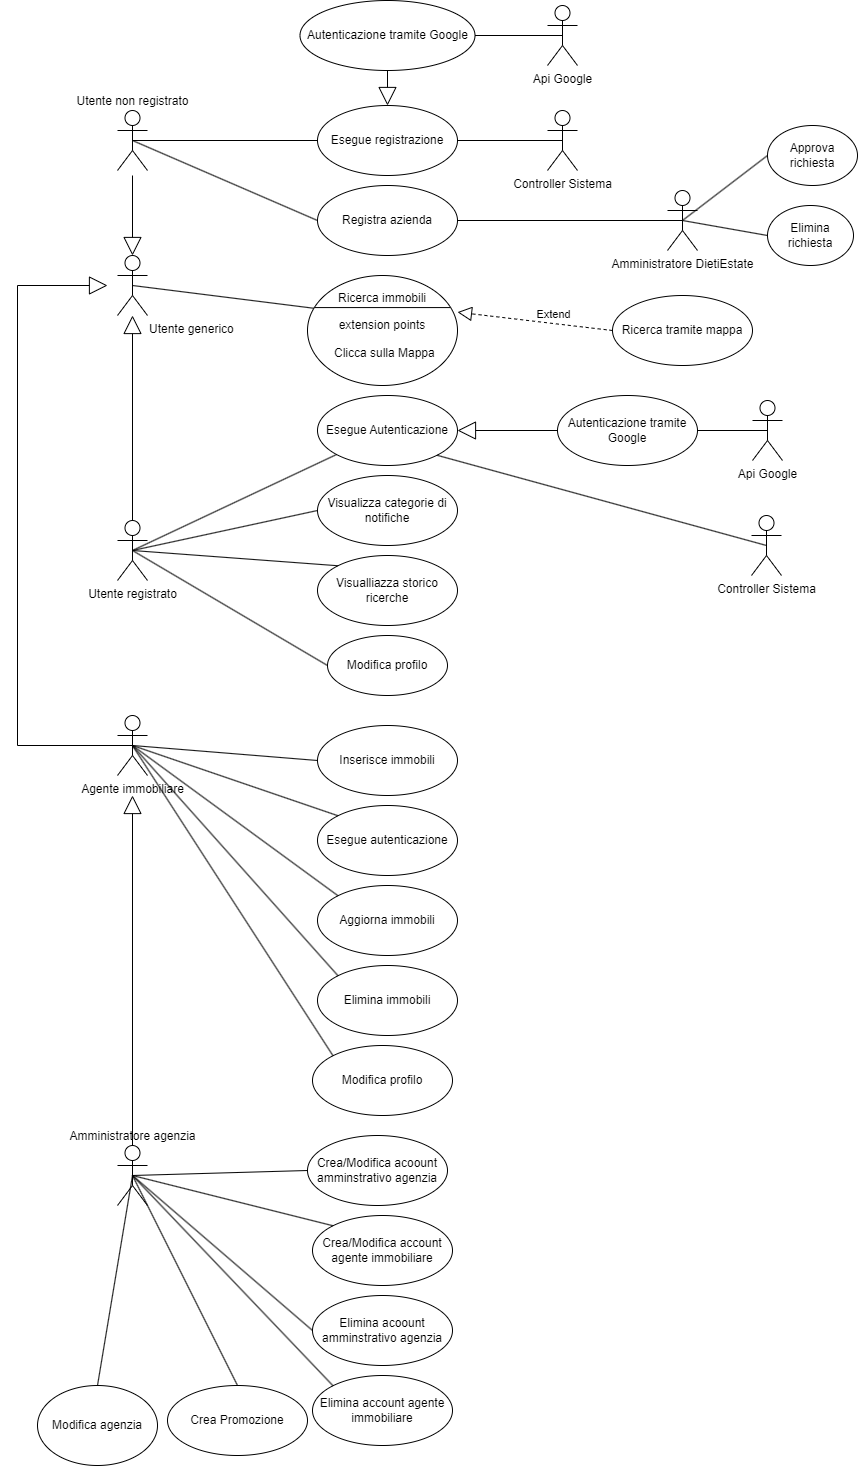
\includegraphics[width=0.73\linewidth]{images/fotoUseCase/UseCaseFinale.png}
    \label{fig:usecase}
\end{figure}
\newpage

\subsection{Diagramma caso d'uso - Utente Generico}
\begin{figure}[H]
    \centering
    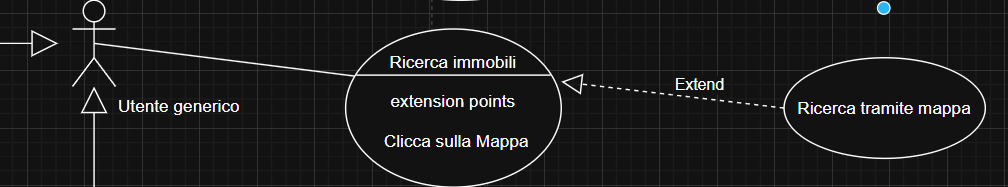
\includegraphics[width=1\linewidth]{images/fotoUseCase/UtenteGenericoUseCase.png}
    \label{fig:usecase}
\end{figure}
Questo diagramma rappresenta le funzionalità accessibili a un utente generico, ovvero a chiunque acceda al sistema senza effettuare il login. In questo caso, l'unica funzionalità disponibile è la ricerca di immobili, che consente agli utenti di esplorare le offerte presenti sulla piattaforma senza dover necessariamente registrarsi o autenticarsi.
\subsubsection{Attori}
\begin{itemize}
    \item \textbf{Attore principale}: Utente generico
    \item \textbf{Attori secondari}: Nessuno
\end{itemize}

\subsection{Diagramma caso d'uso - Utente non registrato}
\begin{figure}[H]
    \centering
    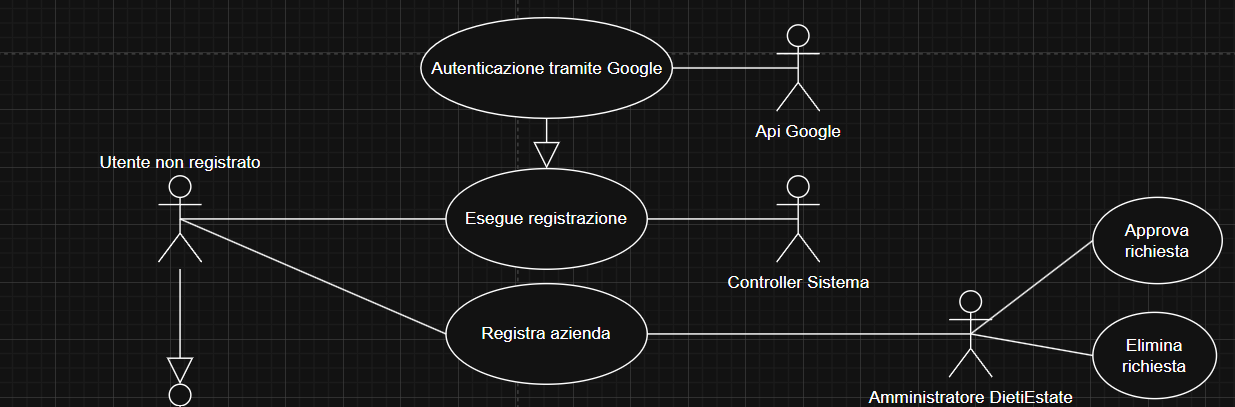
\includegraphics[width=1\linewidth]{images/fotoUseCase/UtenteNonRegistratoUseCase.png}
    \label{fig:usecase}
\end{figure}
Questo diagramma rappresenta le funzionalità accessibili a un utente non registrato, ovvero tutte le funzionalità di un utente generico più la possibilità di registrarsi e di registrare un'azienda. Queste funzionalità consentono agli utenti di creare un account per accedere a funzionalità più avanzate e di registrare un'azienda per gestire le proprie inserzioni immobiliari.
\begin{itemize}
    \item \textbf{Attore principale}: Utente non registrato
    \item \textbf{Attori secondari}: Controller sistema, Api google, Amministratore sistema
    \item \textbf{Eredità da}: Utente generico
\end{itemize}
\newpage

\subsection{Diagramma caso d'uso - Utente registrato}
\begin{figure}[H]
    \centering
    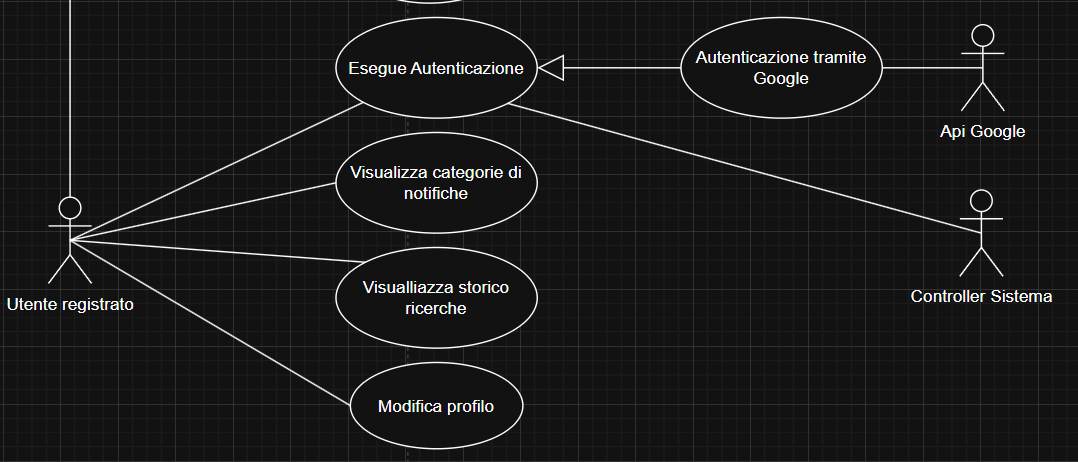
\includegraphics[width=1\linewidth]{images/fotoUseCase/UtenteRegistratoUseCase.png}
    \label{fig:usecase}
\end{figure}
Questo diagramma rappresenta le funzionalità accessibili a un utente registrato, ovvero tutte le funzionalità di un utente generico più la possibilità di accedere a funzionalità avanzate. Queste funzionalità consentono agli utenti di ricevere e gestire le notifiche, visualizzare lo storico delle ricerche e modficare le proprie credenziali.
\begin{itemize}
    \item \textbf{Attore principale}: Utente registrato
    \item \textbf{Attori secondari}: Controller sistema, Api google
    \item \textbf{Eredità da}: Utente generico
\end{itemize}

\subsection{Diagramma caso d'uso - Agente immobiliare}
\begin{figure}[H]
    \centering
    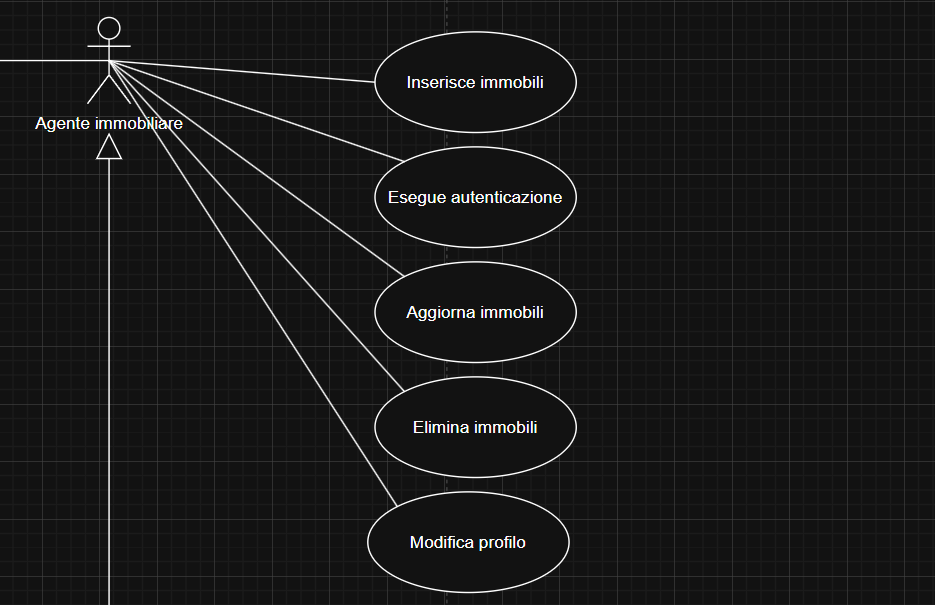
\includegraphics[width=1\linewidth]{images/fotoUseCase/AgenteImmobilirareUseCase.png}
    \label{fig:usecase}
\end{figure}
Questo diagramma rappresenta le funzionalità accessibili a un agente immobiliare, ovvero tutte le funzionalità di un utente generico più la possibilità di inserire e gestire immobili. Queste funzionalità consentono agli agenti immobiliari di caricare, modficare, eliminare immobili nel sistema, inoltre può aggiornare anche le informazioni dell'account.
\begin{itemize}
    \item \textbf{Attore principale}: Agente immobiliare
    \item \textbf{Attori secondari}: Nessuno
    \item \textbf{Eredità da}: Utente generico
\end{itemize}

\subsection{Diagramma caso d'uso - Amministratore agenzia}
\begin{figure}[H]
    \centering
    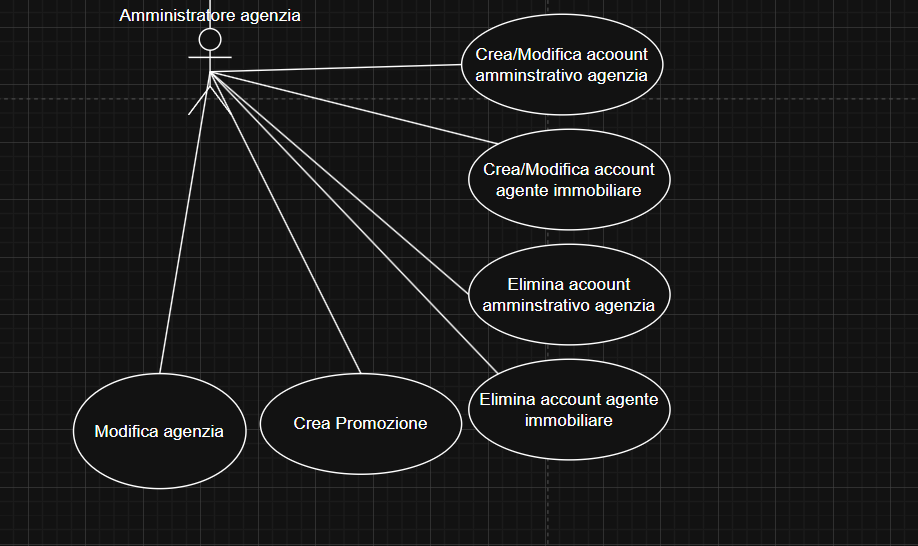
\includegraphics[width=1\linewidth]{images/fotoUseCase/AmministratoreAgenziaUseCase.png}
    \label{fig:usecase}
\end{figure}
Questo diagramma rappresenta le funzionalità accessibili a un amministratore dell'agenzia, ovvero tutte le funzionalità di un agente immobiliare più la possibilità di creare e gestire account, promozioni e l'agenzia. Queste funzionalità consentono agli amministratori di creare e gestire account amministrativi e degli agenti, poter modificare tutte le informazioni dell'agenzia e creare promozioni in una zona specifica dato un'immobile.
\begin{itemize}
    \item \textbf{Attore principale}: Amministratore agenzia
    \item \textbf{Attori secondari}: Nessuno
    \item \textbf{Eredità da}: Agente immobiliare
\end{itemize}

\newpage


\subsubsection{Tabella dei casi d'uso}
\begin{tabularx}{\textwidth}{|>{\raggedright\arraybackslash}X|>{\raggedright\arraybackslash}X|>{\raggedright\arraybackslash}X|}
    \hline
    \textbf{Attore}                               & \textbf{Casi d'uso} & \textbf{Descrizione}                                                                                                                                 \\
    \hline
    Utente non registrato                         &
    \begin{itemize}
        \item Esegue Registrazione
        \item Registra azienda
    \end{itemize}                    &
    Utenti che non hanno ancora un account nel sistema possono registrarsi o registrare una azienda per accedere alle funzionalità.                                                                                            \\
    \hline
    Utente registrato                             &
    \begin{itemize}
        \item Esegue autenticazione
        \item Visualizza storico ricerche
        \item Visualizza categorie di notifiche
        \item Modifica profilo
    \end{itemize}       &
    Gli utenti registrati possono autenticarsi (tramite anche account di terze parti) per accedere ai servizi, gestire notifiche, visualizzare ricerche precedenti, ricevere notifiche rilevanti e modificare il loro profilo. \\
    \hline
    Utente generico                               &
    \begin{itemize}
        \item Ricerca immobile
    \end{itemize}                        &
    Gli utenti possono effettuare ricerche avanzate di immobili utilizzando diversi parametri per individuare proprietà che soddisfano i loro criteri, inoltre possono visualizzare dettagli specifici di ogni immobile.       \\
    \hline
    Agente immobiliare                            &
    \begin{itemize}
        \item Inserisce immobili
        \item Elimina immobili
        \item Esegue autenticazione
        \item Modifica profilo
        \item Aggiorna immobili
    \end{itemize}                   &
    Gli agenti immobiliari possono autenticarsi per caricare immobili nel sistema, aggiornare le informazioni delle proprietà, ed eliminare immobili.                                                                          \\
    \hline
    Amministratore agenzia                        &
    \begin{itemize}
        \item Crea account amministrativo agenzia
        \item Aggiorna account amministrativo agenzia
        \item Elimina account amministrativo agenzia
        \item Crea promozione
        \item Aggiorna informazioni agenzia
        \item Crea account agente immobiliare
        \item Aggiorna account agente immobiliare
        \item Elimina account agente immobiliare
    \end{itemize} &
    Gli amministratori dell'agenzia possono creare e gestire account amministrativi e degli agenti, aggiornare le informazioni dell'agenzia e creare promozioni.                                                               \\
    \hline
\end{tabularx}

\newpage
\subsection{Personas}
Le \textit{Personas} di riferimento per delineare i requisiti funzionali e di usabilità del sistema. La scelta dei profili è stata guidata dalla necessità di rappresentare scenari d'uso estremamente eterogenei, garantendo che il software possa rispondere efficacemente a diverse categorie di utenti.

I casi analizzati di seguito sono stati selezionati per coprire un ampio spettro di target:
\begin{itemize}
    \item \textbf{Utenti privati con diverse competenze digitali:} dall'utente senior che necessita di estrema semplicità, al genitore focalizzato su parametri logistici e familiari.
    \item \textbf{Profili professionali e tecnici:} soggetti che richiedono strumenti avanzati di monitoraggio, rapidità di esecuzione e funzionalità specifiche per il mercato immobiliare e degli investimenti.
\end{itemize}

Tale diversificazione permette di validare l'architettura del software sotto molteplici punti di vista, assicurando un'esperienza d'uso inclusiva e performante per ogni tipologia di utente finale.

\begin{figure}[H]
    \centering
    
\includegraphics[width=1\linewidth]{images/Personas1.jpg}
    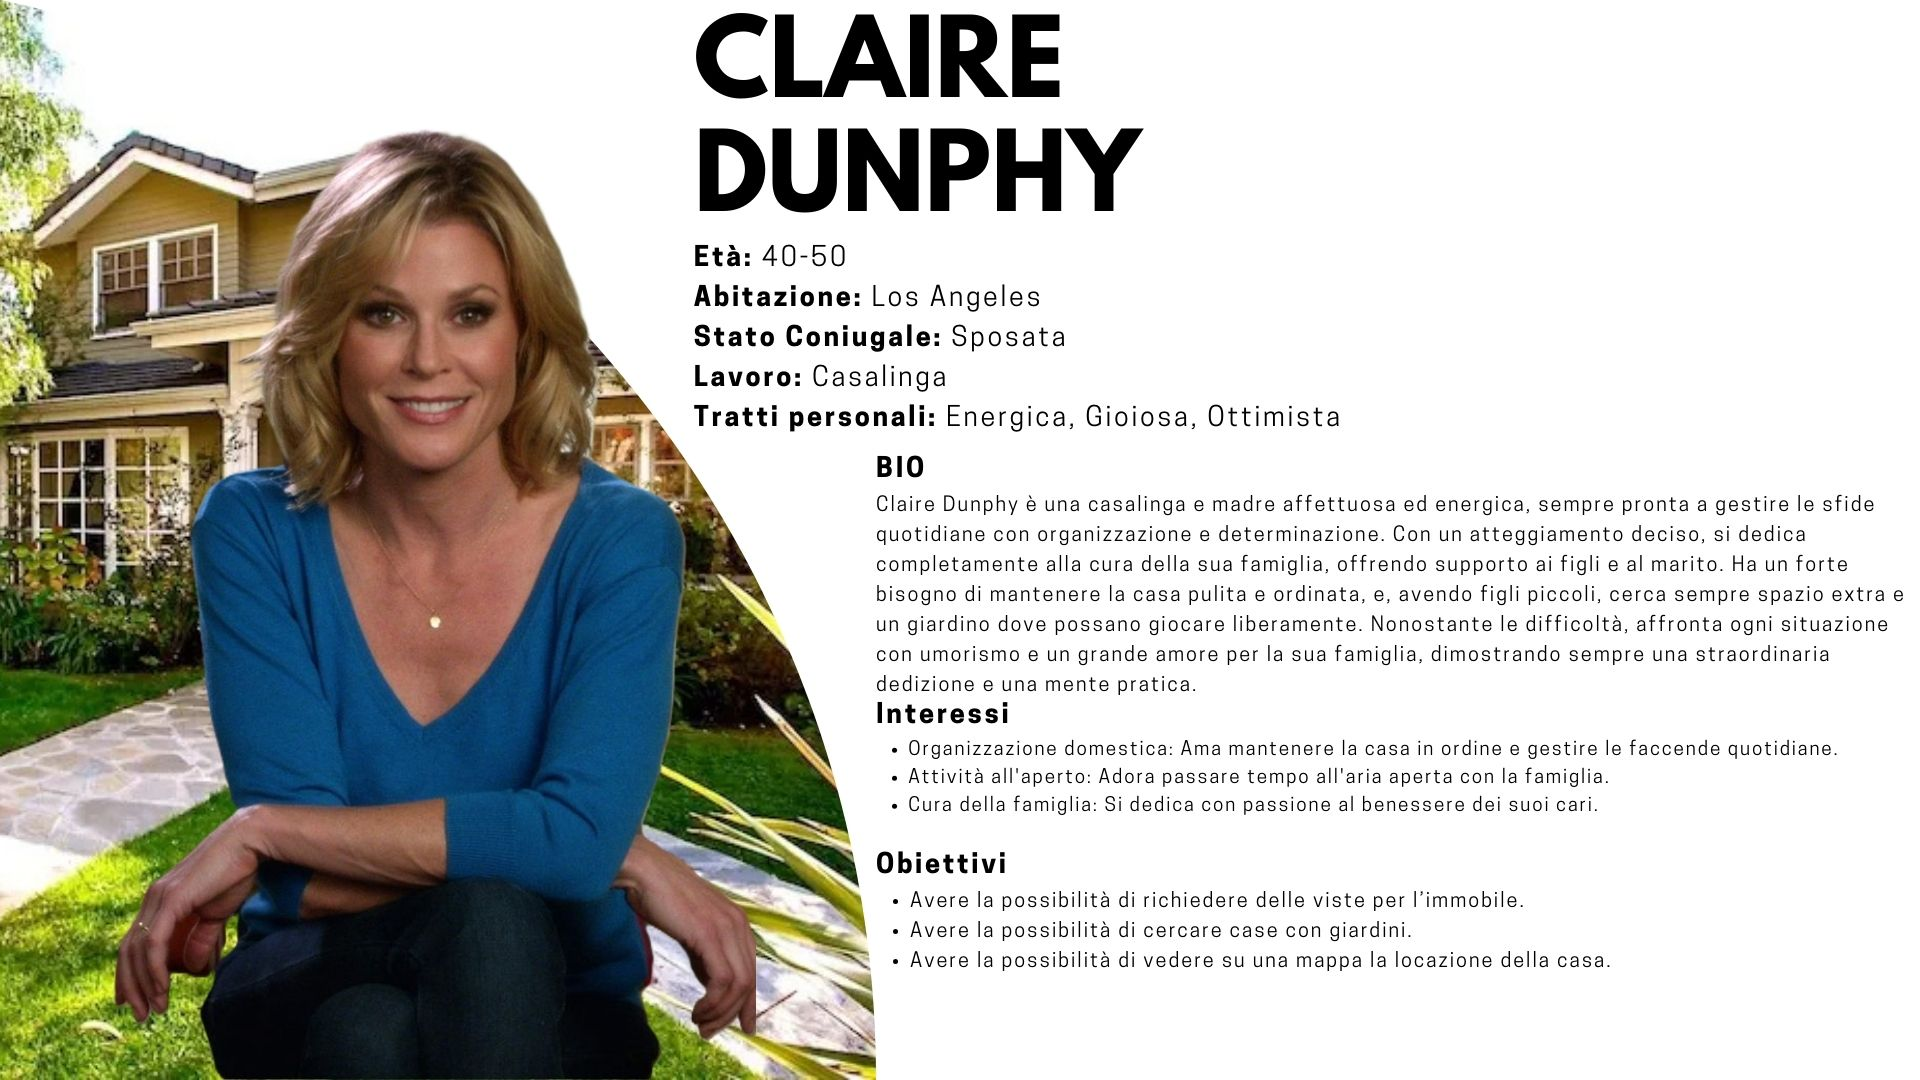
\includegraphics[width=1\linewidth]{images/Personas2.jpg}
    \label{fig:usecase}
\end{figure}

\begin{figure}[H]
    \centering
    
\includegraphics[width=1\linewidth]{images/Personas3.jpg}
    
\includegraphics[width=1\linewidth]{images/Personas4.jpg}
    \label{fig:usecase}
\end{figure}


\newpage
\subsection{Descrizione testuale strutturate dei casi d'uso}
In questa sezione vengono analizzati alcuni casi d'uso utilizzando la notazione tabellare proposta da Alistair Cockburn, al fine di rappresentare in modo chiaro e strutturato le interazioni tra gli utenti e il sistema. Per supportare e rendere più immediata la comprensione delle tabelle, sono stati inoltre realizzati dei mock-up a bassa fedeltà che illustrano visivamente i principali scenari d’uso.

\subsubsection{Cockburn caso uso: Ricerca immobile}
\begin{figure}[H]
    \centering
    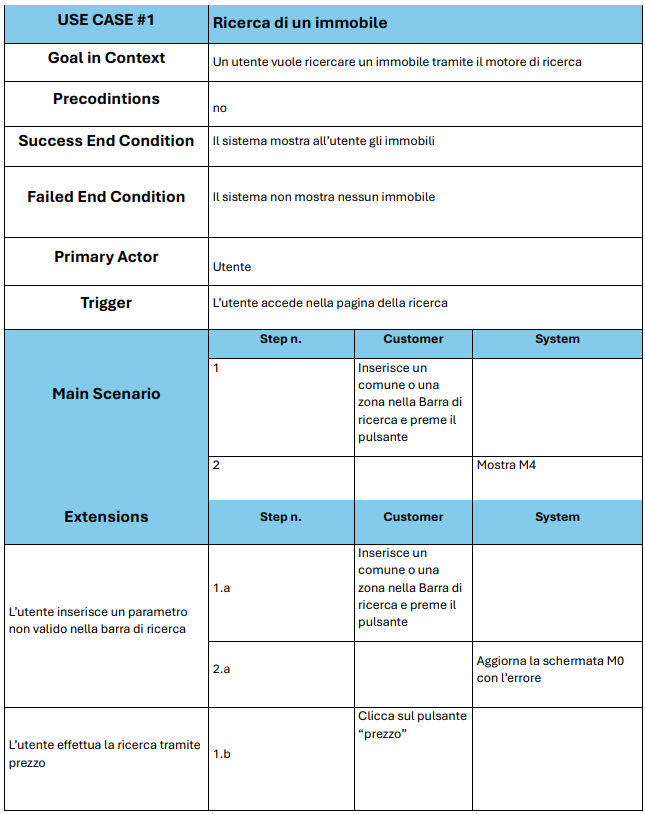
\includegraphics[width=0.73\linewidth]{images/CockBurnRicercaImmobile.png}
    \label{fig:usecase}
\end{figure}
\begin{figure}[H]
    \centering
    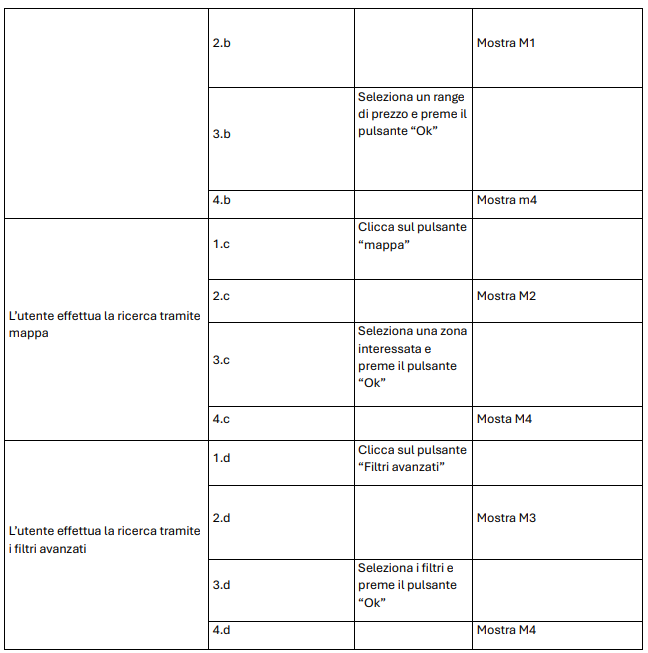
\includegraphics[width=0.73\linewidth]{images/CockBurnRicercaImmobile2.png}
    \label{fig:usecase}
\end{figure}
\newpage
\subsubsection{Cockburn caso uso: Caricamento di un immobile}
\begin{figure}[H]
    \centering
    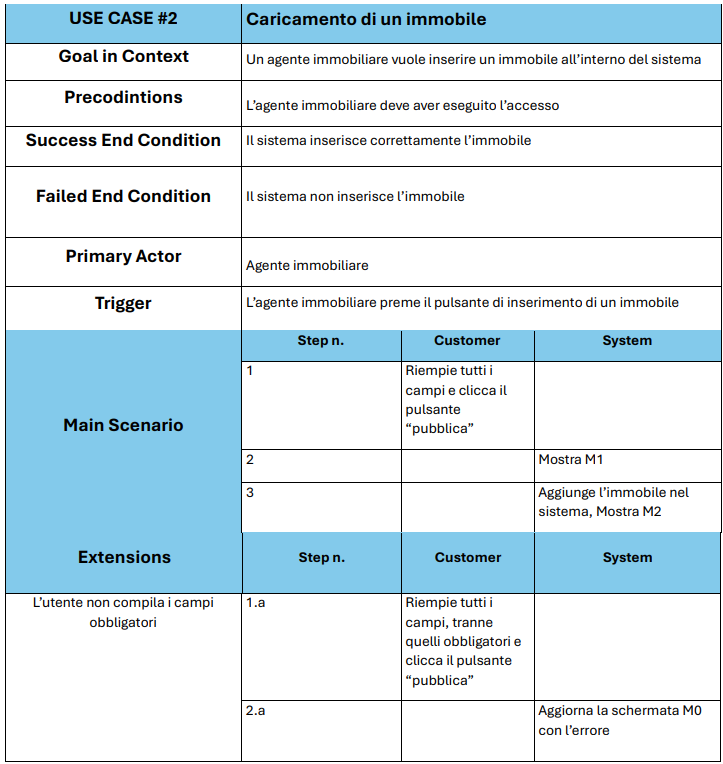
\includegraphics[width=0.73\linewidth]{images/CockBurnCaricamentoImmobile.png}
    \label{fig:usecase}
\end{figure}\textbf{}
\newpage
\subsubsection{Cockburn caso uso: Aggiornamento di un immobile}
\begin{figure}[H]
    \centering
    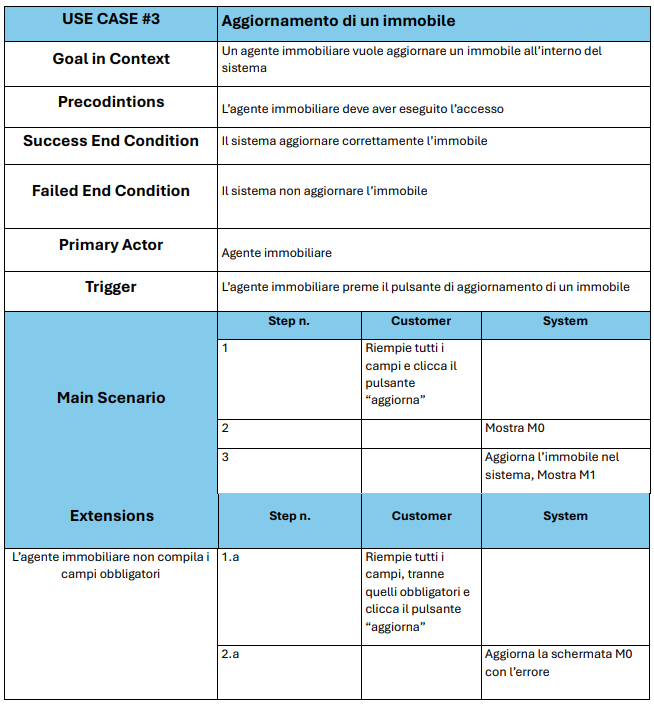
\includegraphics[width=0.73\linewidth]{images/CockBurnAggiornamentoImmobile.png}
    \label{fig:usecase}
\end{figure}
\newpage
\subsubsection{Cockburn caso uso: Creazione account agente immobiliare}
\begin{figure}[H]
    \centering
    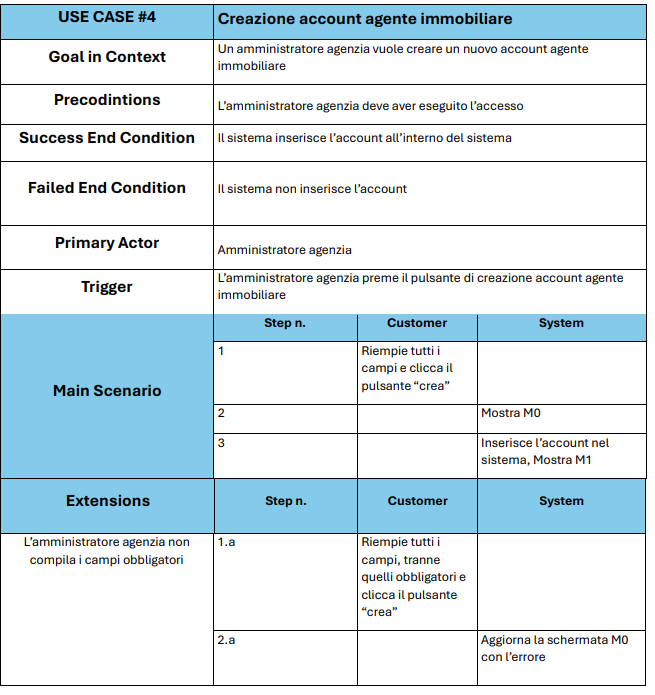
\includegraphics[width=0.73\linewidth]{images/CockBurnCreazioneAgente.png}
    \label{fig:usecase}
\end{figure}

\newpage


\subsection{Introduzione Mockup a bassa fedeltà}
Il seguente parte del documento descrive le funzionalità e l'interfaccia delle varie pagine che compongono il mockup del portale immobiliare \textbf{DietiEstate24}. Ogni sezione analizza una specifica vista, illustrandone lo scopo e i componenti principali attraverso l'analisi dei mockup tecnici forniti.

\subsection{Homepage}
La pagina principale del portale funge da punto di ingresso per gli utenti. Offre un'interfaccia chiara per avviare rapidamente una ricerca o navigare verso altre sezioni.

\textbf{Funzionalità principali:}
\begin{itemize}
    \item \textbf{Barra di navigazione superiore (Header):} Contiene i collegamenti alle sezioni principali (``Annunci'', ``Vendi'', ``Agenzie'') e i pulsanti per l'autenticazione (``Accedi'', ``Registrati'').
    \item \textbf{Hero Section e Motore di Ricerca:} Un'area prominente dove l'utente può inserire la località desiderata e selezionare il prezzo massimo tramite un menu a tendina.
    \item \textbf{Anteprima Mappa Interattiva Generator:} Un modulo per la visualizzazione geografica degli immobili.
    \item \textbf{Vetrina Immobili in Evidenza:} Una griglia dinamica che mostra le ``migliori offerte di oggi'', sotto forma di card cliccabili contenenti l'immagine, il prezzo, il titolo, l'indirizzo e i dettagli sintetici (locali, bagni, quadratura).
\end{itemize}

\begin{figure}[H]
    \centering
    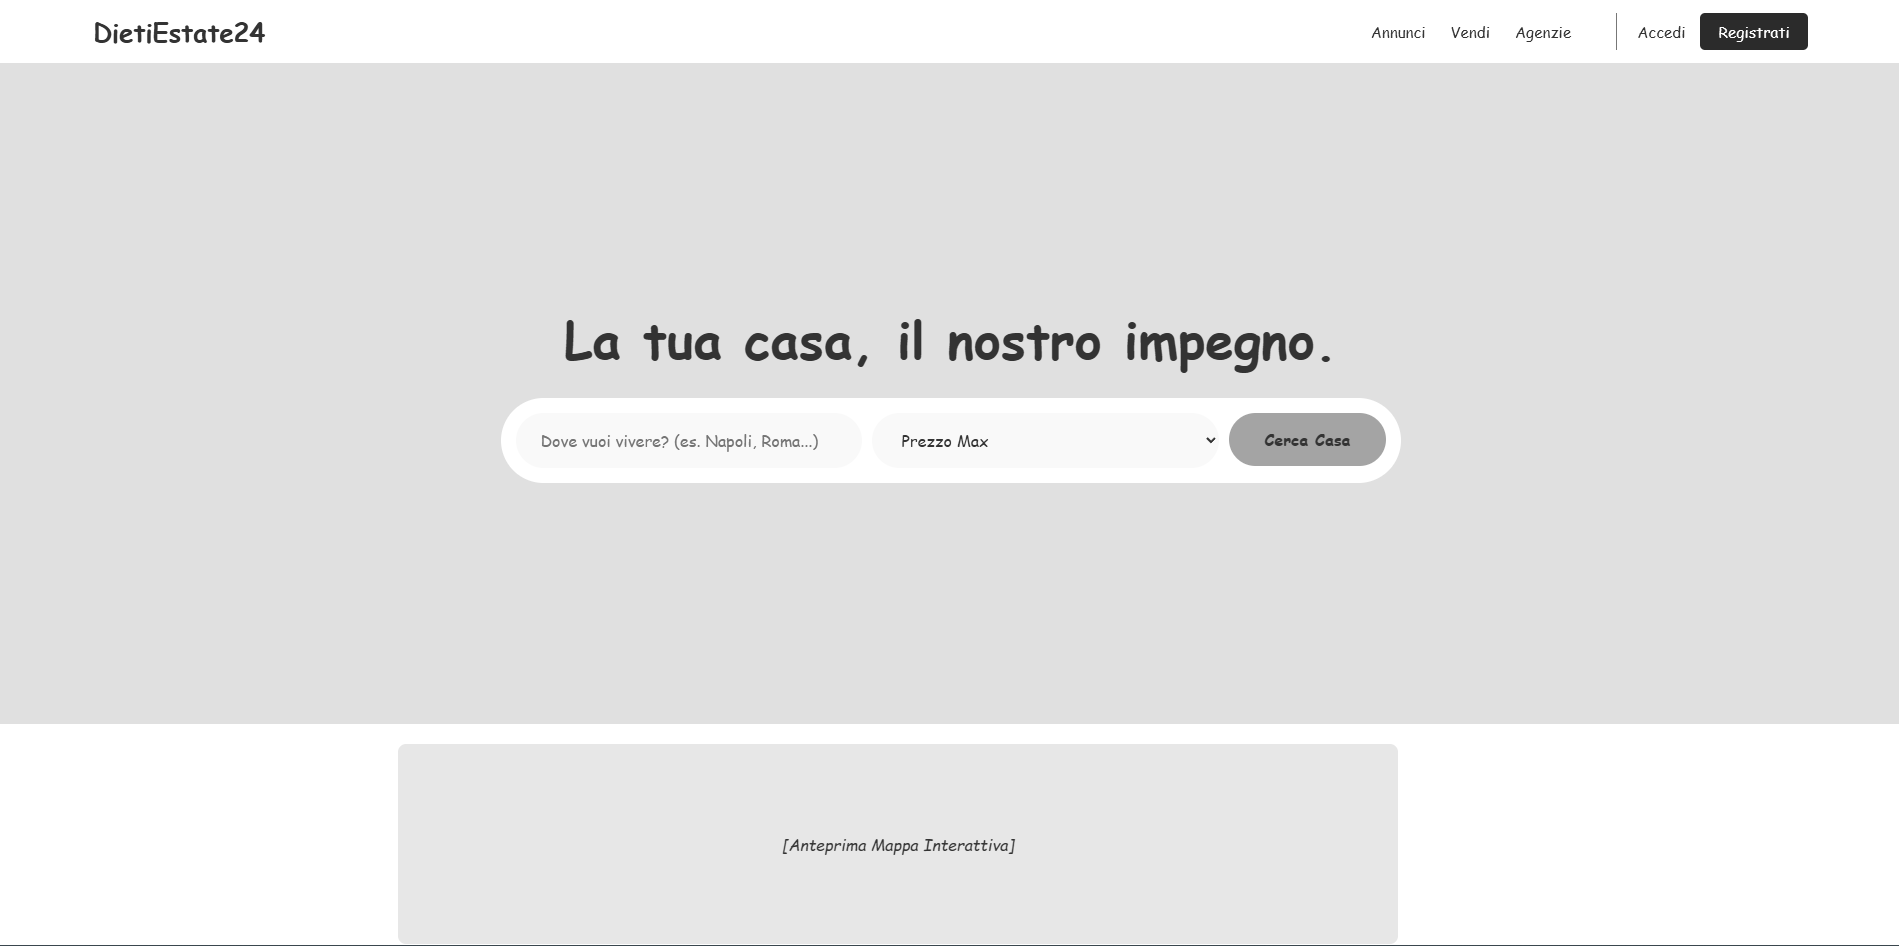
\includegraphics[width=0.8\textwidth]{images/fotomockup/index/1.png}
    \caption{Homepage vista 1}
\end{figure}

\begin{figure}[H]
    \centering
    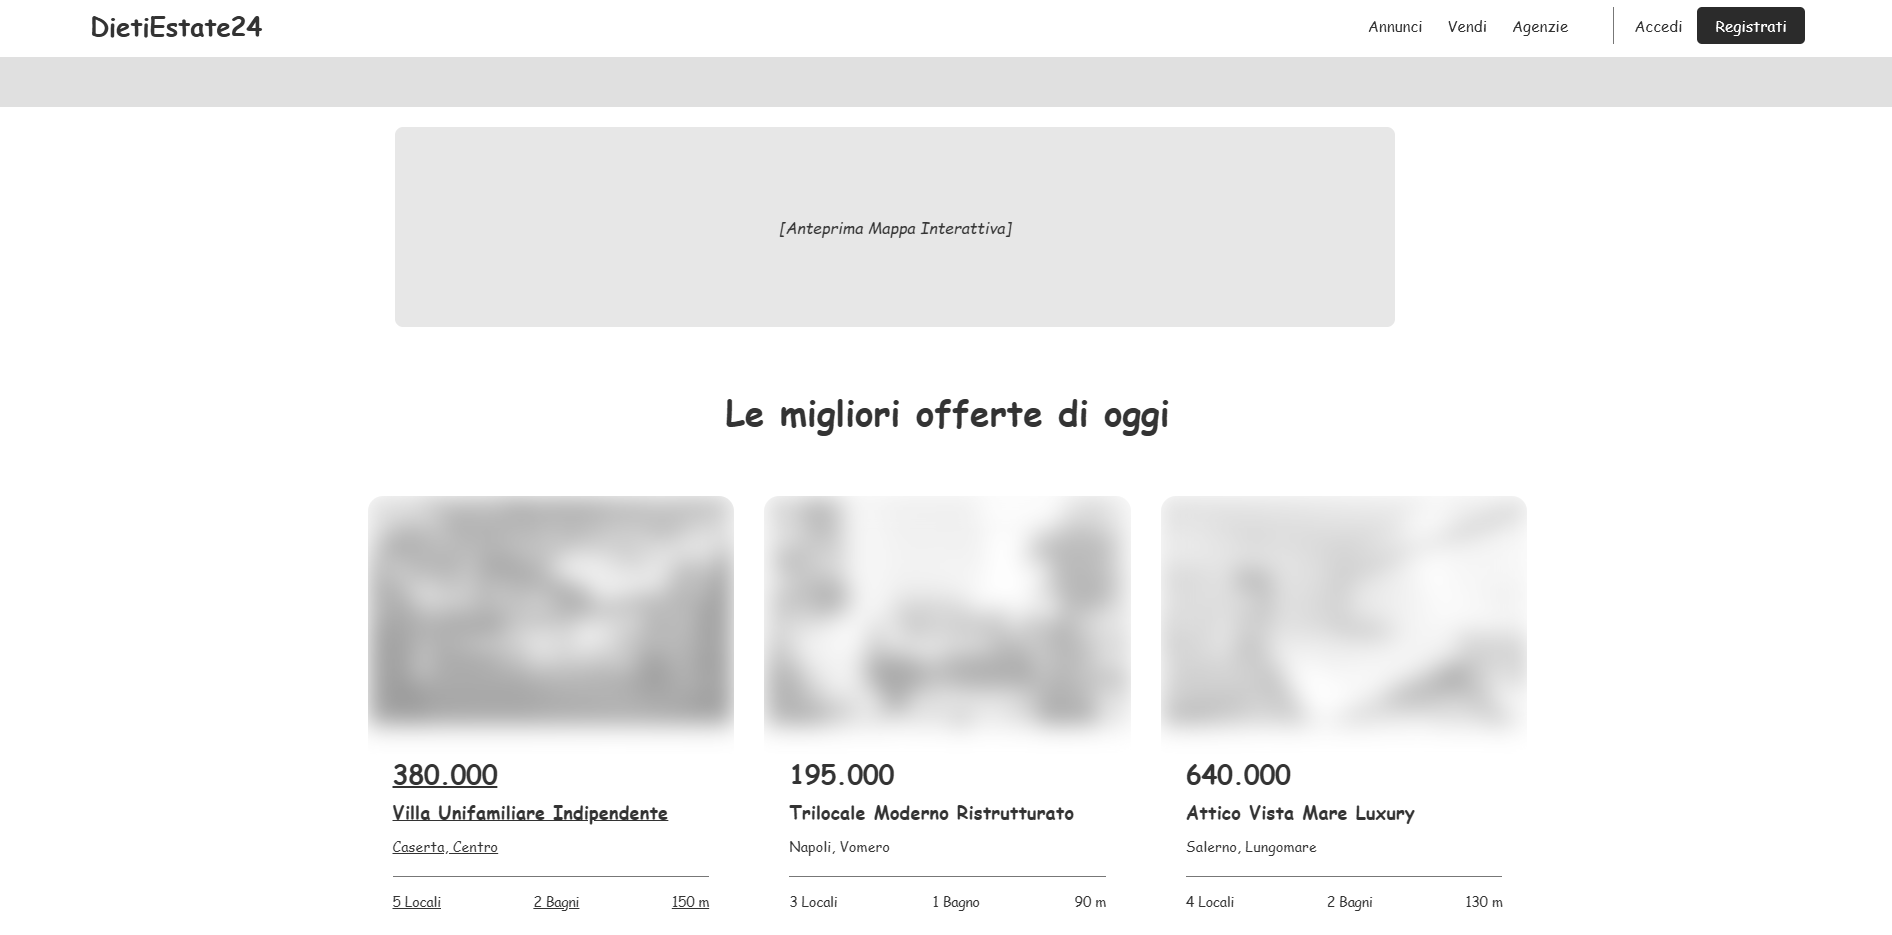
\includegraphics[width=0.8\textwidth]{images/fotomockup/index/2.png}
    \caption{Homepage vista 2}
\end{figure}


\subsection{Pagina di Ricerca}
Accessibile sia dalla homepage che dalla barra di navigazione, questa pagina presenta i risultati della ricerca e permette di affinarli tramite filtri avanzati.

\textbf{Funzionalità principali:}
\begin{itemize}
    \item \textbf{Sidebar Filtri Avanzati:} Permette di filtrare i risultati per Località, Tipologia (Appartamento, Villa, Rustico, Ufficio), Prezzo Massimo (tramite slider interattivo) e Caratteristiche specifiche (Balcone, Posto Auto, ecc.).
    \item \textbf{Ordinamento Risultati:} Menu a tendina per ordinare la lista (Più recenti, Prezzo crescente/decrescente, Superficie).
    \item \textbf{Griglia Risultati:} Mostra le card degli immobili corrispondenti ai criteri di ricerca, con eventuali badge personalizzati (es. ``In Evidenza'').
\end{itemize}

\begin{figure}[H]
    \centering
    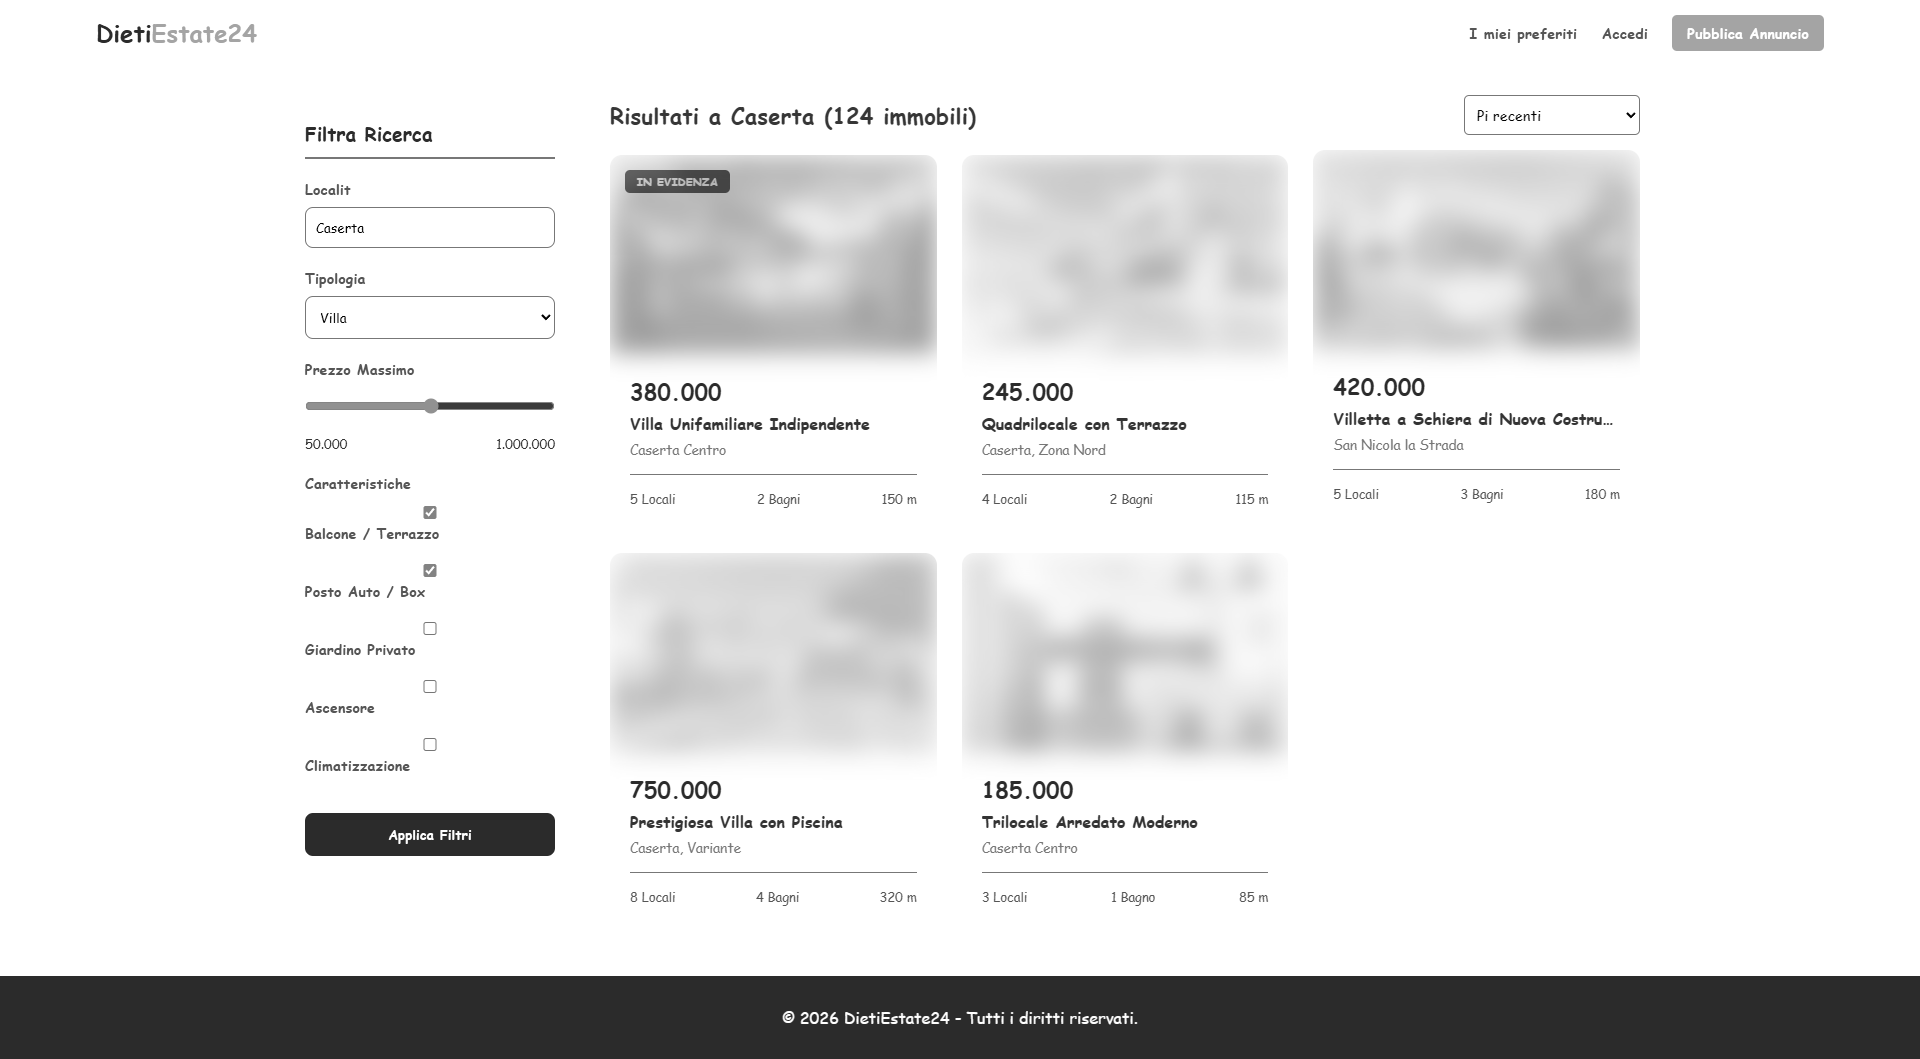
\includegraphics[width=0.8\textwidth]{images/fotomockup/Ricerca.png}
    \caption{Ricerca Immobili}
\end{figure}

\newpage
\subsection{Dettaglio Immobile}
Questa vista fornisce tutte le informazioni dettagliate relative a uno specifico immobile selezionato dall'utente.

\textbf{Funzionalità principali:}
\begin{itemize}
    \item \textbf{Galleria Media:} Un layout a griglia asimmetrica che mostra l'immagine principale e delle anteprime per scorrere gli spazi interni ed esterni della casa.
    \item \textbf{Scheda Informativa:} Riassume il prezzo, il badge dello stato (es. ``In Vendita''), il titolo dell'annuncio e l'indirizzo esatto.
    \item \textbf{Griglia Caratteristiche:} Indicatori numerici e iconografici rapidi per Locali, Bagni, Metratura e Classe Energetica.
    \item \textbf{Sidebar di Contatto:} Una scheda fissa (sticky) con form rapido per email e pulsante integrato per contatto diretto su WhatsApp.
\end{itemize}

\begin{figure}[H]
    \centering
    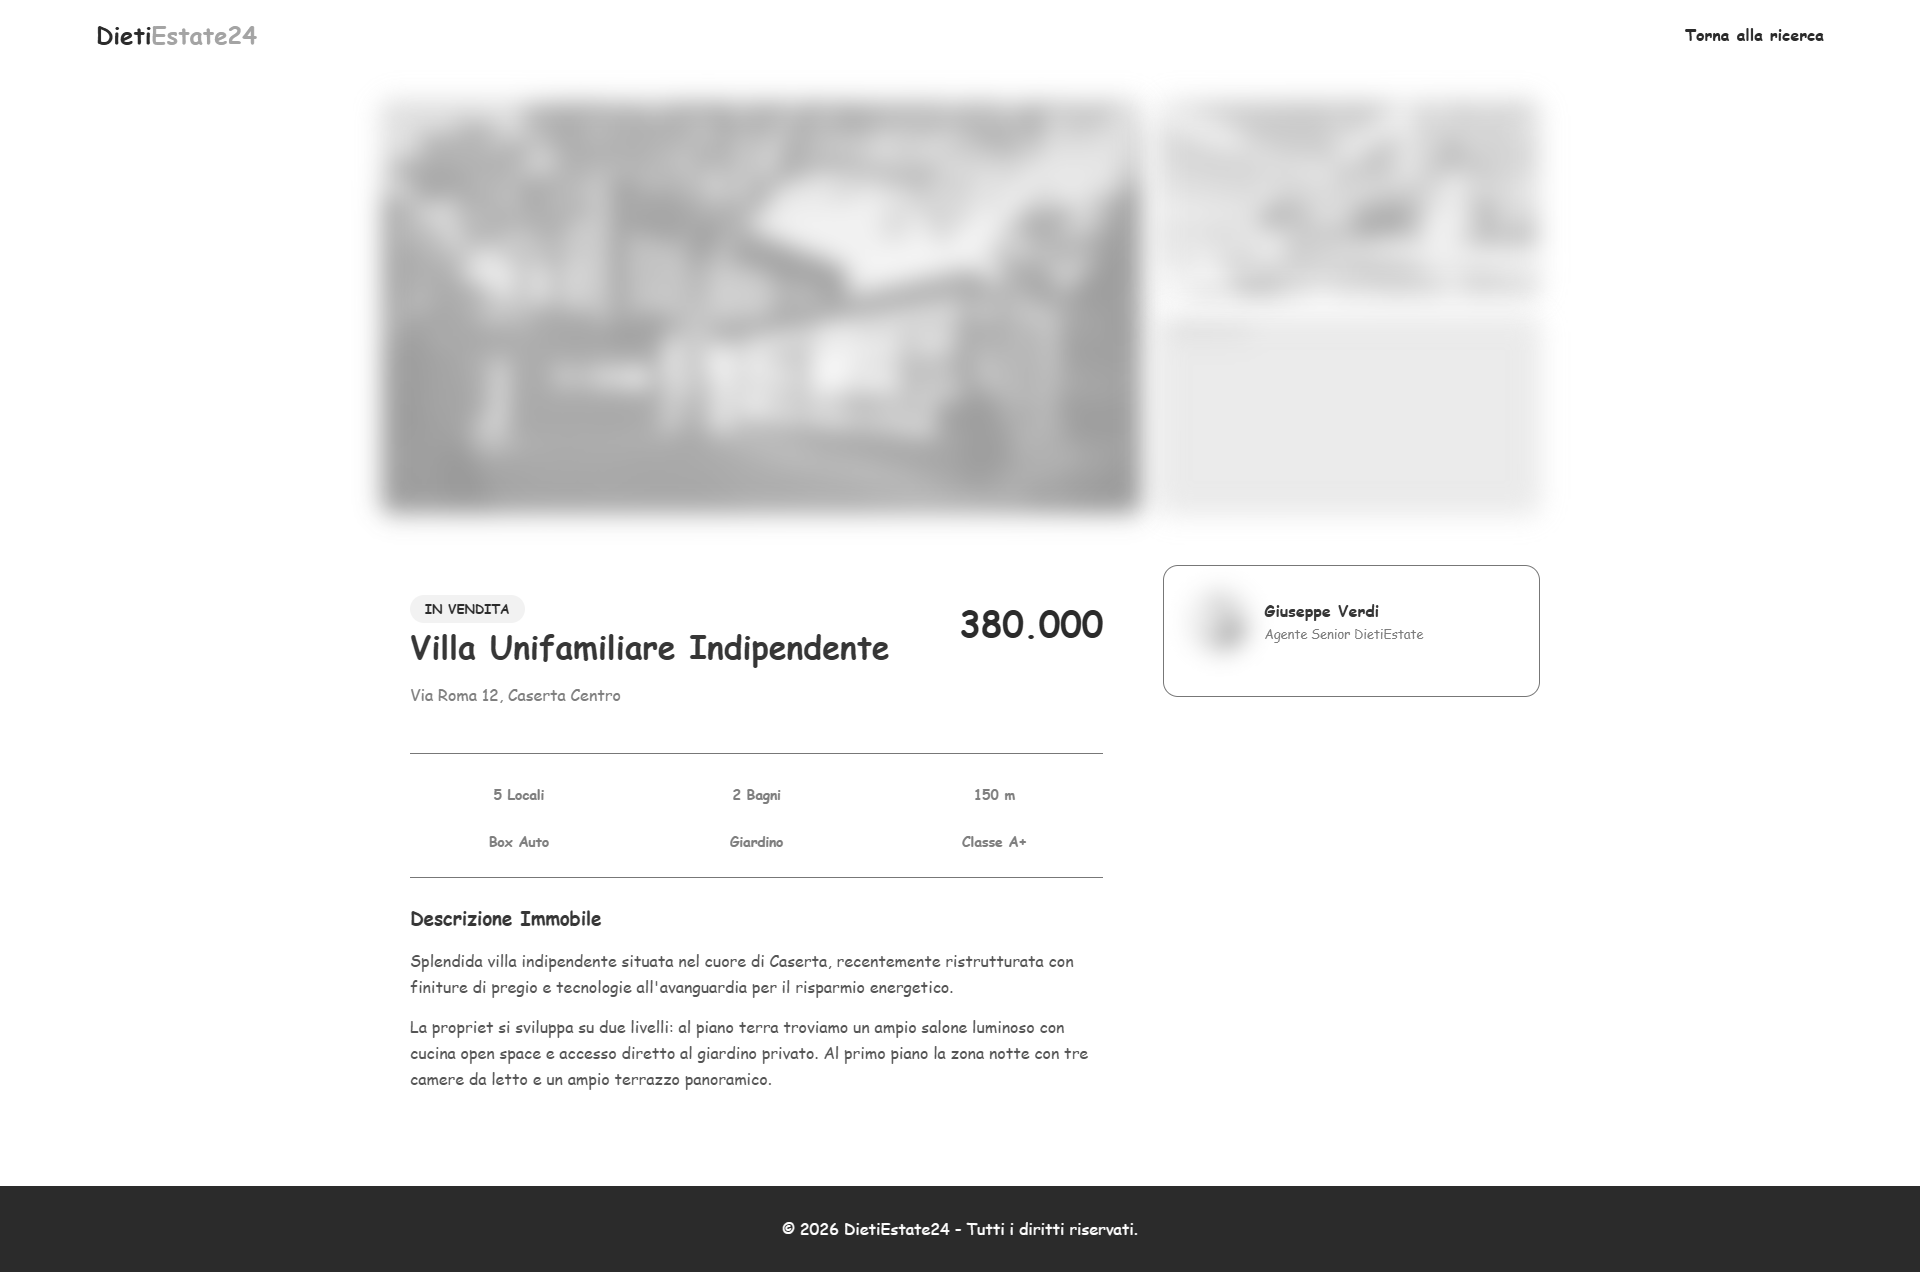
\includegraphics[width=0.8\textwidth]{images/fotomockup/visualizzazione immobile.png}
    \caption{Dettaglio Immobile}
\end{figure}
\newpage
\subsection{Pagina Agenzia Immobiliare}
Rappresenta la vetrina pubblica di un'agenzia immobiliare registrata sul portale DietiEstate24.

\textbf{Funzionalità principali:}
\begin{itemize}
    \item \textbf{Hero Banner dell'Agenzia:} Presenta logo, nome, indirizzo e statistiche chiave (totale immobili, anni di attività, feedback medio).
    \item \textbf{Schede di Navigazione Interne:} Permettono di filtrare il portafoglio tra immobili ``In Vendita'', ``In Affitto'' o ``Venduti''.
    \item \textbf{Sidebar Contatti e Team:} Offre bottoni rapidi per contattare l'ufficio e documenta la composizione del team aziendale.
\end{itemize}

\begin{figure}[H]
    \centering
    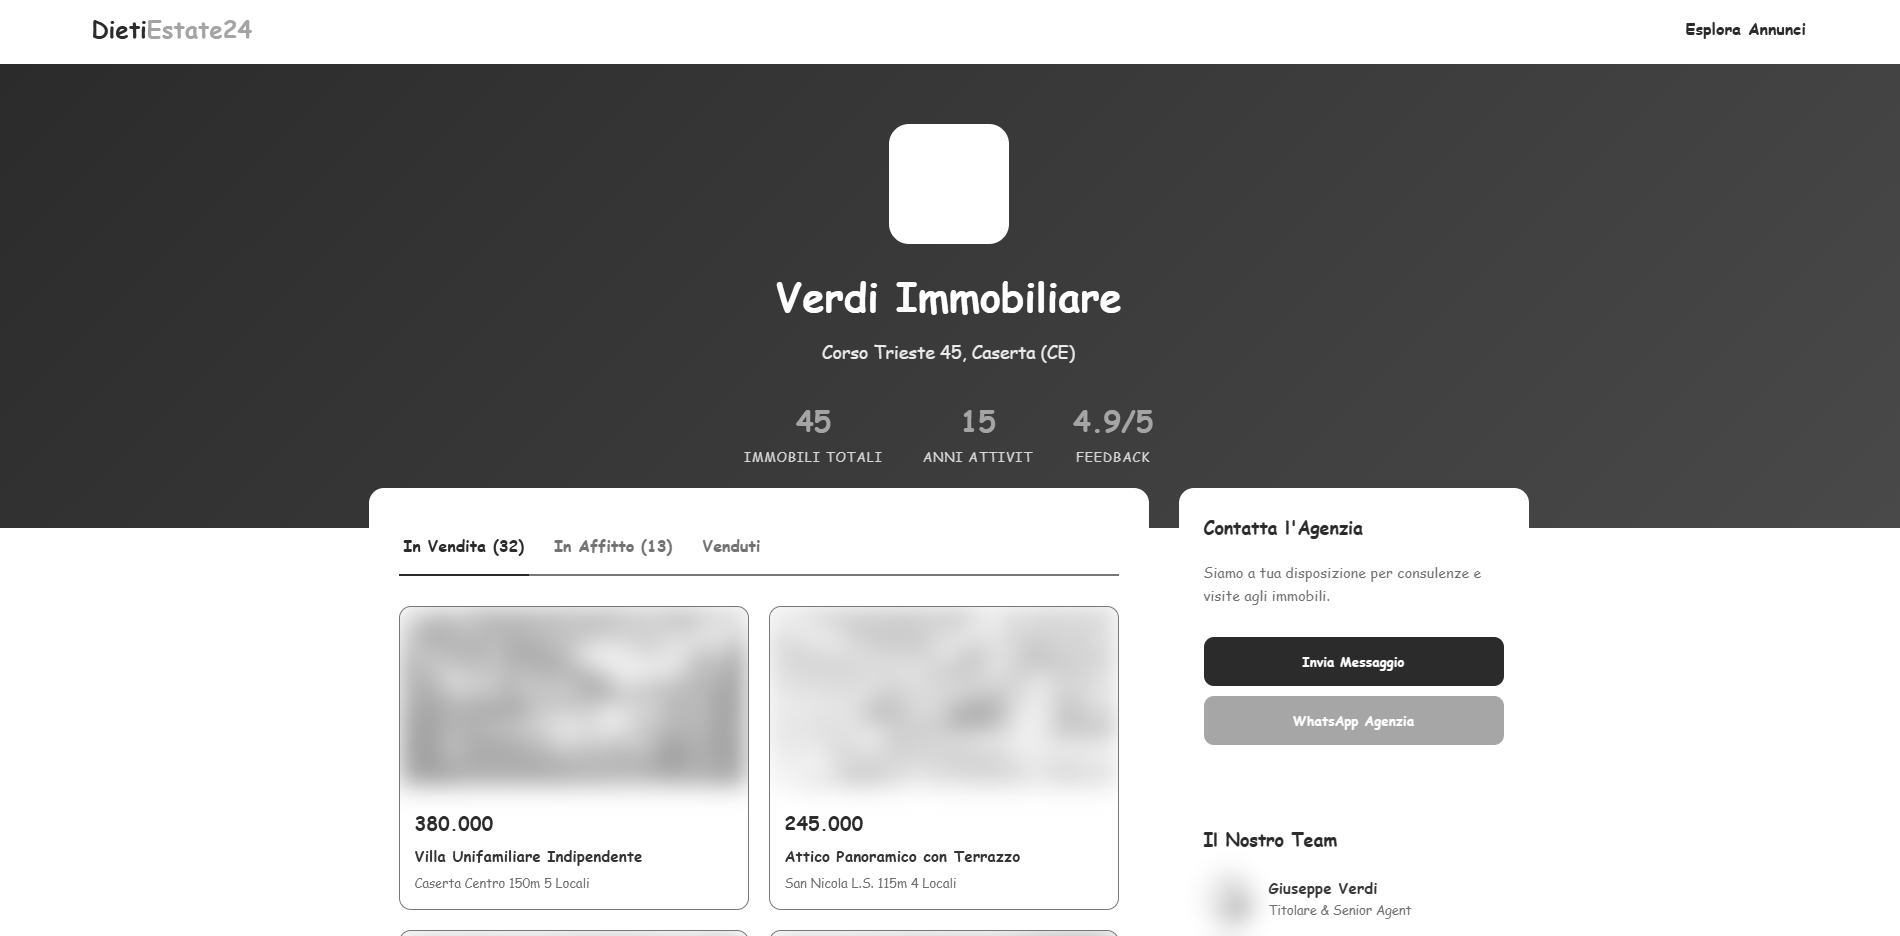
\includegraphics[width=0.8\textwidth]{images/fotomockup/mia agenzia/3.png}
    \caption{Profilo Agenzia vista 1}
\end{figure}

\newpage
\subsection{Inserimento Immobile}
Dedicata agli utenti registrati o agli agenti per la pubblicazione di nuovi annunci immobiliari.

\textbf{Funzionalità principali:}
\begin{itemize}
    \item \textbf{Form Modulare:} Suddiviso in sezioni tematiche chiare (Informazioni di base, Posizione, Caratteristiche).
    \item \textbf{Mappa Interattiva Integrata:} Per indicare e confermare visivamente la posizione della proprietà.
    \item \textbf{Area Upload Media:} Finestra drag \& drop per caricare le immagini dell'immobile.
    \item \textbf{Gestione Bozza:} Opzione per salvare il lavoro e riprenderlo in seguito.
\end{itemize}

\begin{figure}[H]
    \centering
    
\includegraphics[width=0.8\textwidth]{images/fotomockup/inserimento  immobile/screencapture-file-C-Users-giggi-Desktop-DieitiEstateFrontEnd-aggiuntaImmobile-html-2026-03-16-17_07_54.png}
    \caption{Inserimento Immobile}
\end{figure}

\newpage
\subsection{Accesso e Registrazione}
Pagine standard per la gestione dell'identità e l'autenticazione degli utenti.

\textbf{Funzionalità principali:}
\begin{itemize}
    \item \textbf{Login:} Form di autenticazione standard e SSO (Single Sign-On) tramite Google e Facebook.
    \item \textbf{Registrazione:} Raccolta dati anagrafici, accettazione privacy e supporto alla registrazione social.
\end{itemize}

\begin{figure}[H]
    \centering
    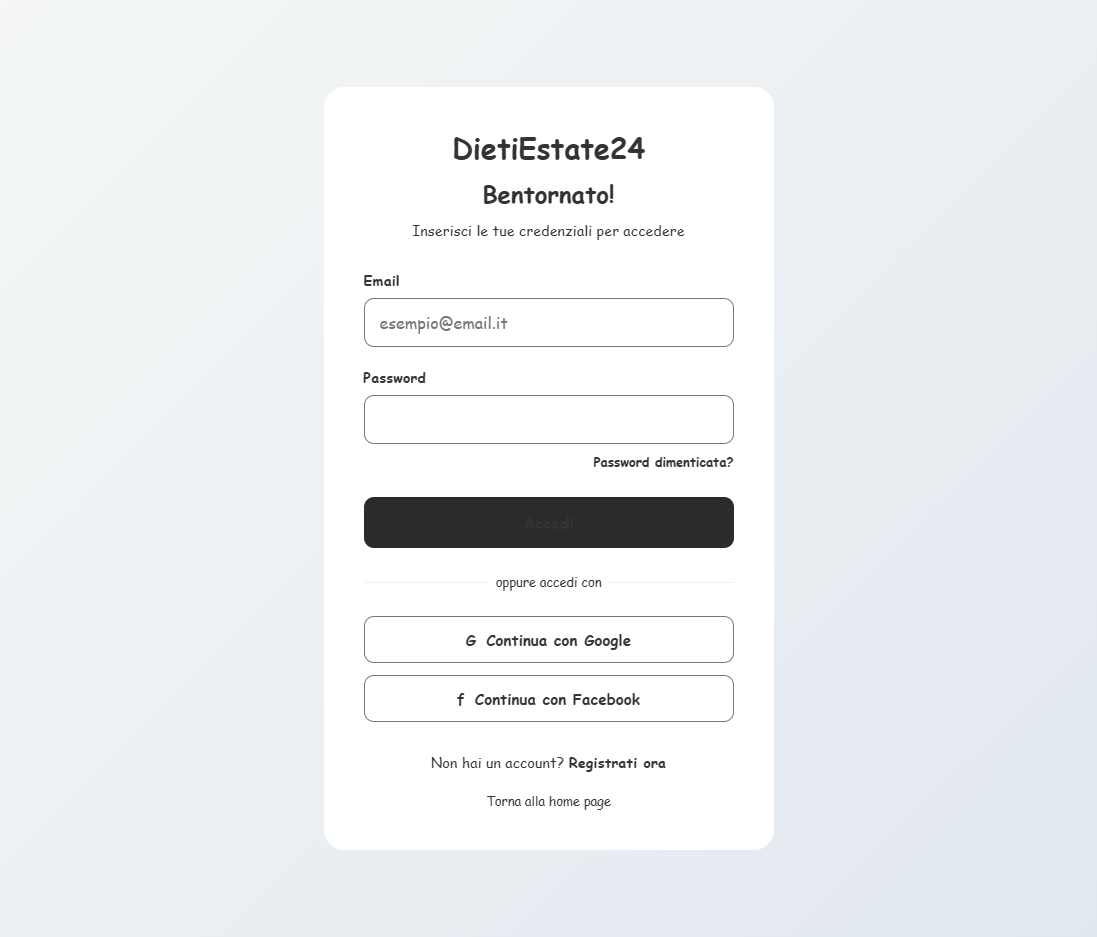
\includegraphics[width=0.6\textwidth]{images/fotomockup/login.png}
    \caption{Mockup Login}
\end{figure}

\begin{figure}[H]
    \centering
    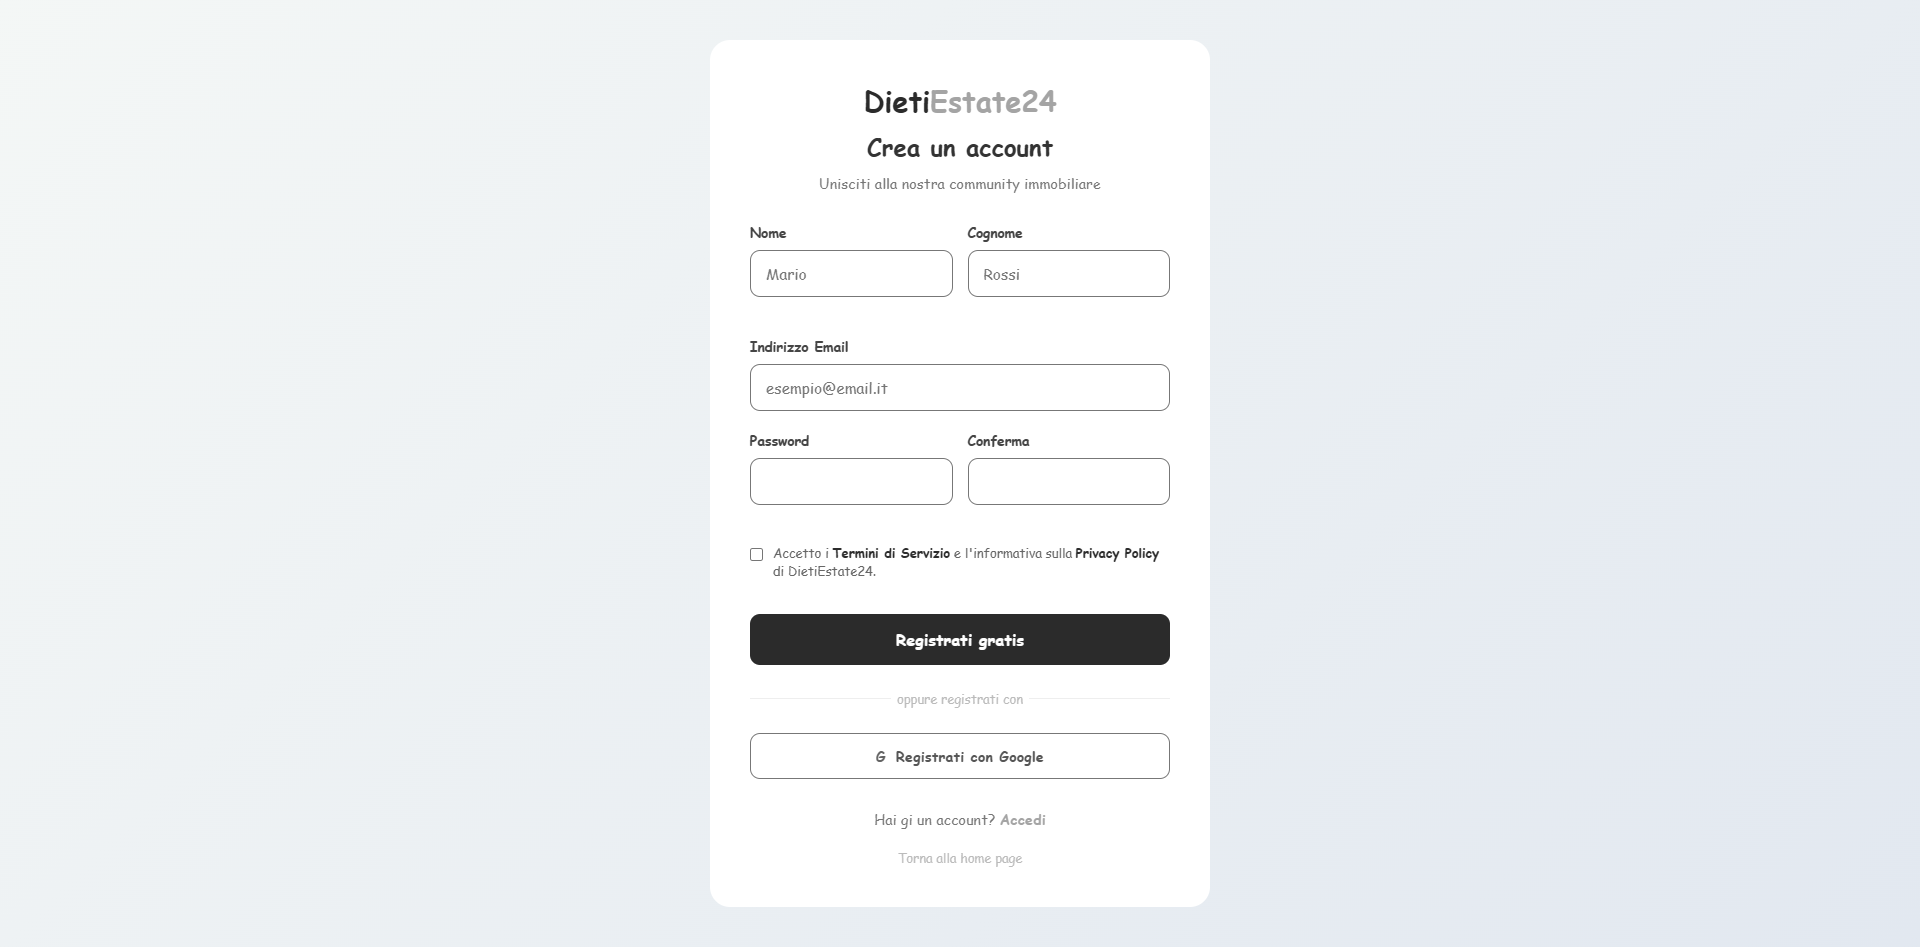
\includegraphics[width=0.6\textwidth]{images/fotomockup/registrazione.png}
    \caption{Mockup Registrazione}
\end{figure}

\newpage
\subsection{Pannelli di Profilo}
Il portale gestisce l'area riservata in base alla tipologia di account.

\subsection{Profilo Utente Privato}
\textbf{Funzionalità:} Sidebar di navigazione personale, form di modifica informazioni e feed attività recente per ritrovare immobili salvati.

\begin{figure}[H]
    \centering
    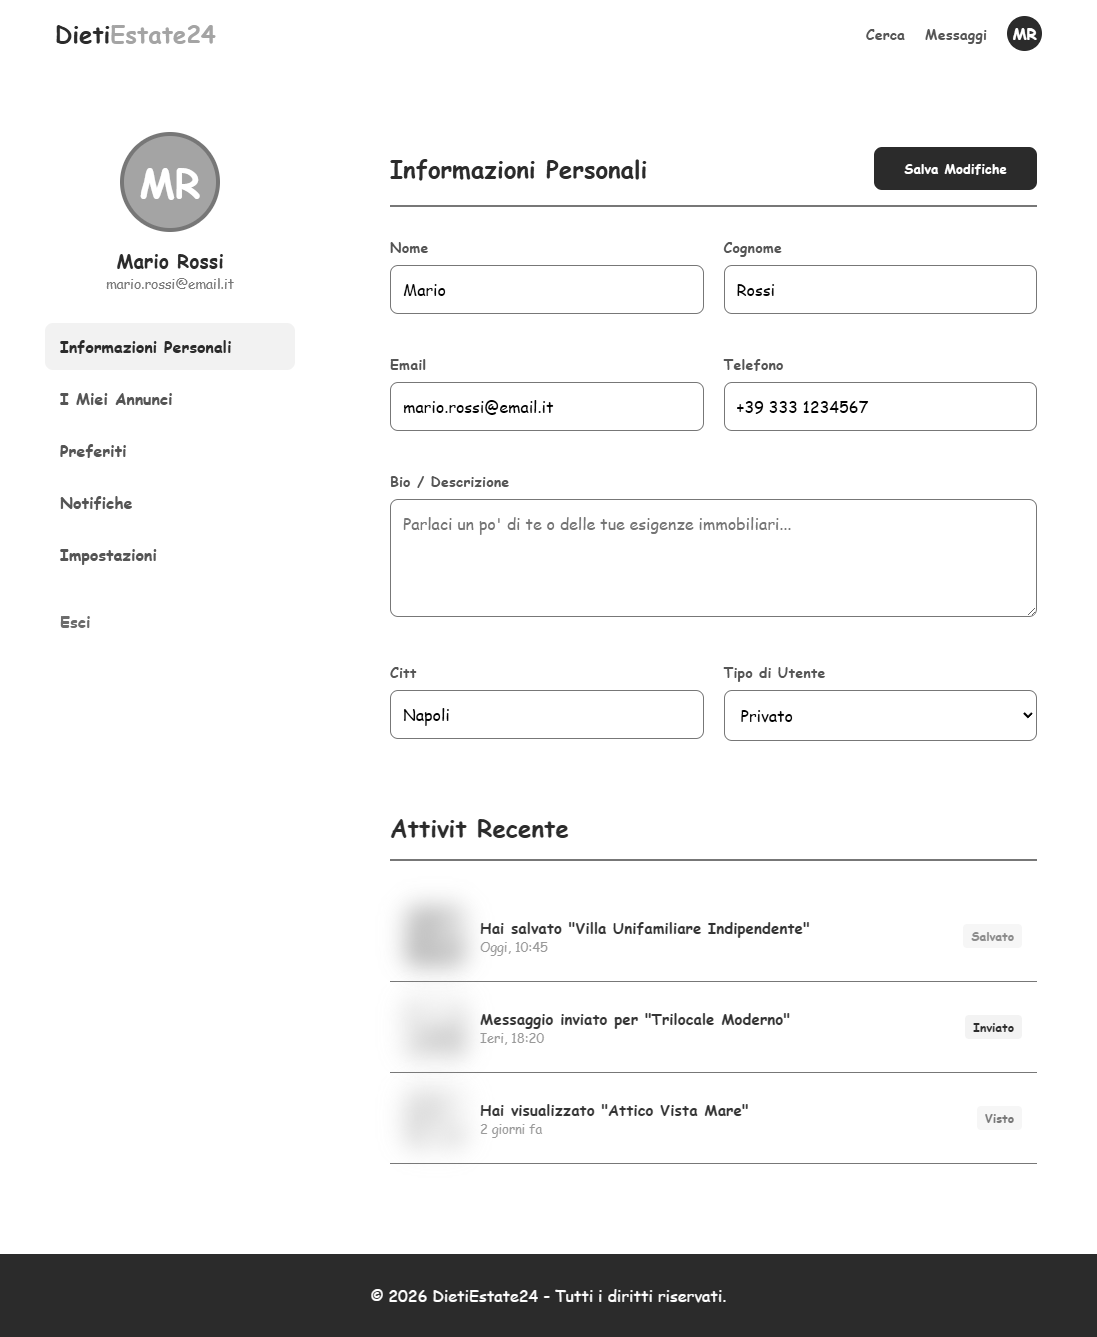
\includegraphics[width=0.8\textwidth]{images/fotomockup/profilo utente.png}
    \caption{Profilo Utente Privato}
\end{figure}

\newpage
\subsection{Profilo Agente}
\textbf{Funzionalità:} Dashboard con statistiche Quick View, gestione dati professionali e billing, gestione del portafoglio (modifica/disattivazione annunci).

\begin{figure}[H]
    \centering
    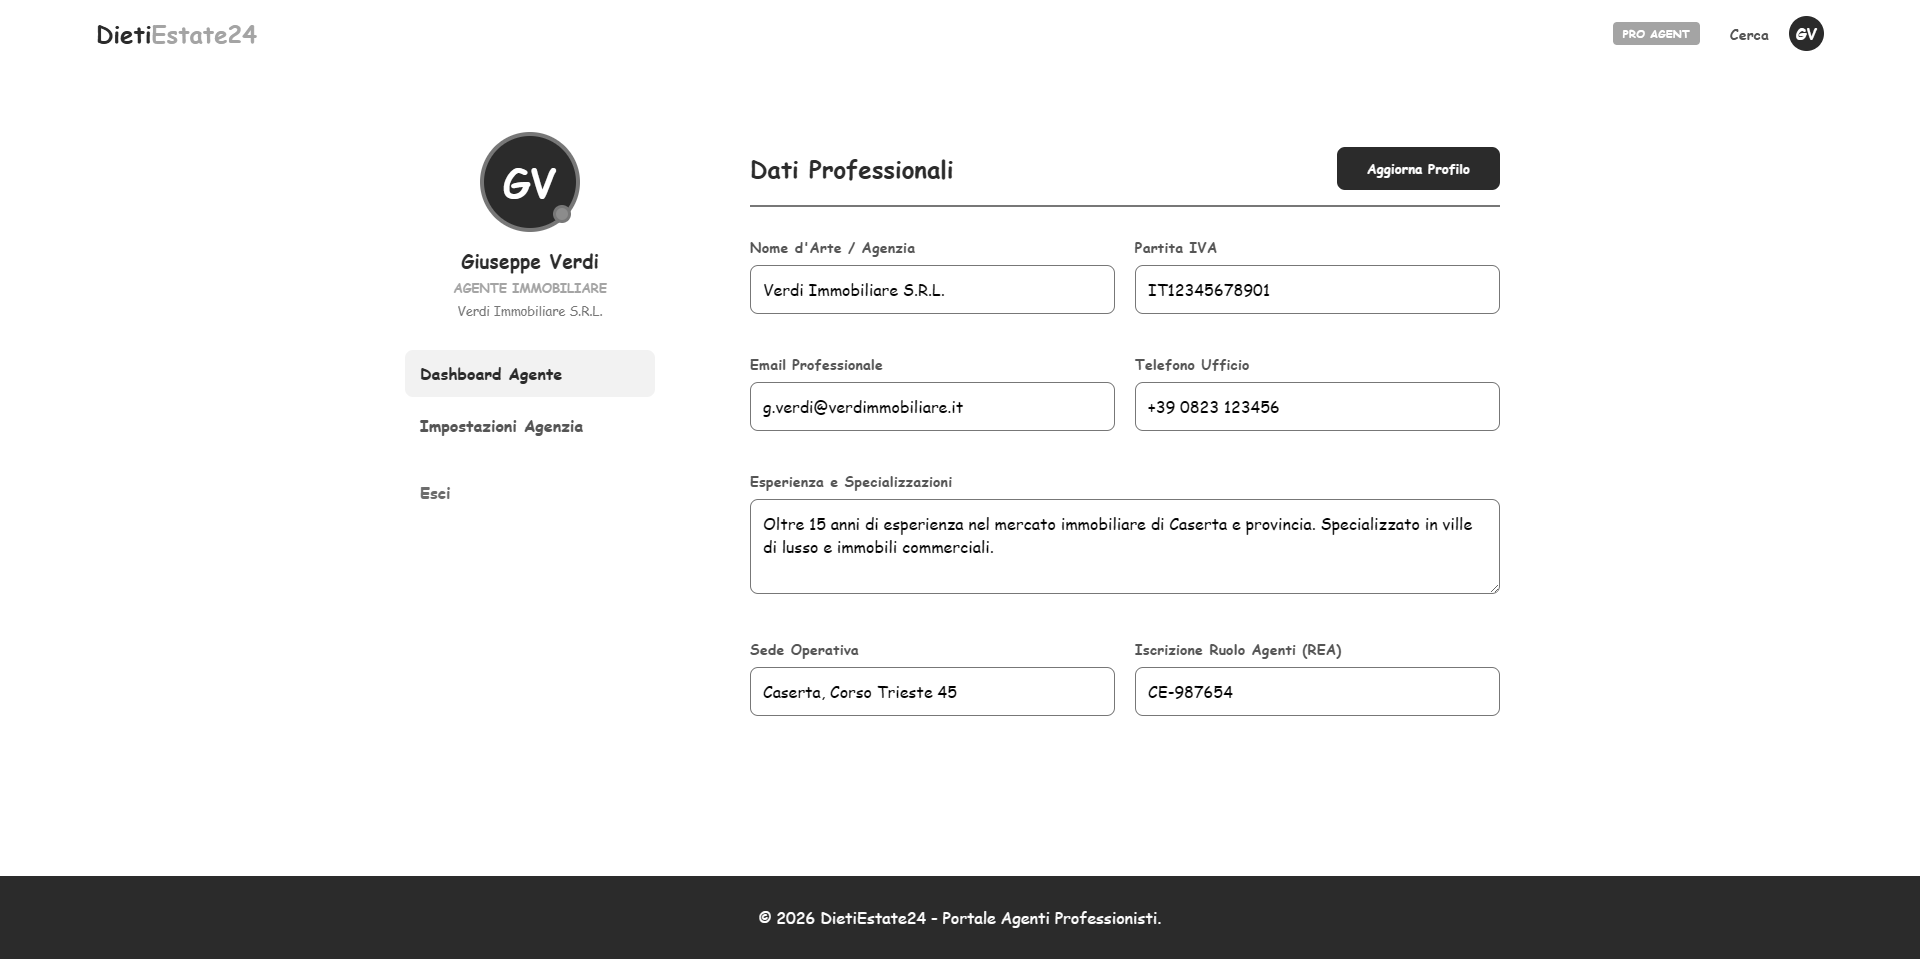
\includegraphics[width=0.8\textwidth]{images/fotomockup/profilo agente.png}
    \caption{Profilo Agente}
\end{figure}







\newpage
\subsection{Descrizione dei requisiti non funzionali e di dominio}
Nella presente sezione saranno individuati e illustrati in modo dettagliato i requisiti non funzionali e di dominio. I requisiti non funzionali rappresentano le specifiche che indicano il modo in cui il sistema deve operare, delineando le proprietà e la qualità del sistema stesso. I requisiti di dominio stabiliscono le regole, i vincoli e le peculiarità del contesto in cui il sistema è attivo, nello specifico il settore immobiliare.

\subsubsection{Requisiti non funzionali}
I requisiti non funzionali possono essere distinti in:\begin{enumerate}

    \item \textbf{Requisiti di prodotto}:\begin{itemize}
              \item \textbf{Usabilità}: \begin{enumerate}
                        \item L'interfaccia dovrebbe essere facile da usare e accessibile a tutti gli utenti.
                        \item Il sistema deve permettere l'utilizzo di app di terze parti (Facebook, Google, GitHub) per semplificare il processo di registrazione e accesso.
                    \end{enumerate}
              \item \textbf{Prestazioni}: \begin{enumerate}
                        \item Il sistema dovrebbe assicurare tempi di risposta inferiori a 3 secondi per operazioni comuni come la ricerca di immobili e il caricamento delle pagine.
                        \item La ricerca con filtri avanzati dovrebbe fornire i risultati in meno di 5 secondi, anche quando vengono applicati numerosi filtri.
                    \end{enumerate}
              \item \textbf{Sicurezza}: \begin{enumerate}
                        \item Il sistema dovrebbe supportare diversi livelli di accesso (Amministratori di agenzia, Agenti immobiliari).
                        \item Le password devono essere salvate nel database utilizzando algoritmi di hashing.
                        \item Il sistema deve impedire attacchi SQL Injection.
                    \end{enumerate}
              \item \textbf{Affidabilità}: \begin{enumerate}
                        \item È necessario che il sistema assicuri un uptime del 99,9% per minimizzare le interruzioni del servizio.
                    \end{enumerate}
              \item \textbf{Scalabilità}: \begin{enumerate}
                        \item Il sistema dovrebbe supportare la distribuzione su server cloud scalabili come AWS e Azure.
                    \end{enumerate}
              \item \textbf{Manutenibilità}: \begin{enumerate}
                        \item Il codice dovrebbe essere modulare per semplificare l'integrazione di nuove funzionalità.
                    \end{enumerate}
          \end{itemize}
    \item \textbf{Requisiti organizzativi}: \begin{enumerate}
              \item Il sistema dev'essere costruito come un sistema distribuito composto da due componenti principali: Back-end e Front-end.
              \item Dev'essere sviluppato usando linguaggi di programmazione Object-Oriented.
          \end{enumerate}
\end{enumerate}

\newpage
\subsubsection{Requisiti di Dominio}
In seguito verranno elencati i vari requisiti di dominio
\begin{enumerate}
    \item \textbf{Pubblicazione di annunci immobiliari}: Gli agenti immobiliari devono avere la capacità di caricare dettagli sugli immobili, dove ciascuno deve essere completamente descritto. Le informazioni necessarie includono il prezzo, le dimensioni, l'indirizzo, le fotografie, una breve descrizione, il piano, e vari servizi (come portineria, climatizzazione e così via).
    \item \textbf{Ricerca avanzata degli immobili}: I beni immobili possono essere trovati tramite filtri avanzati che consentono di specificare parametri quali la tipologia dell'annuncio, il range di prezzo, il numero di stanze, la classe energetica e la posizione geografica (ricerca per comune o città).
    \item \textbf{Cronologia delle ricerche}: Gli utenti devono poter consultare lo storico delle ricerche eseguite. Ogni volta che un utente effettua una ricerca, il sistema deve registrare la ricerca.
    \item \textbf{Notifiche per gli utenti}: Gli utenti devono ricevere notifiche relative a nuove proprietà in linea con le loro ricerche recenti (basate sull'area selezionata) e messaggi promozionali. Gli utenti devono anche avere la possibilità di visualizzare singolarmente le categorie di notifiche.
    \item \textbf{Ricerca e visualizzazione degli immobili sulla mappa}: Gli utenti possono trovare gli immobili attraverso una mappa interattiva che consente di selezionare un'area e cercare proprietà nell'area selezionata. Inoltre, gli immobili devono essere visualizzati sulla mappa.
    \item \textbf{Gestione dei Ruoli e dei Permessi}: Il sistema deve supportare una gerarchia di ruoli specifica del settore immobiliare, con diversi livelli di accesso.
\end{enumerate}
\newpage

\section{Design del sistema}
Una volta completata l’acquisizione e l’analisi dei requisiti, è necessario tradurre il dominio dei requisiti nel dominio del sistema, definendo l'architettura e le tecnologie da adottare.
Il primo passo consiste nella selezione dell'architettura più adeguata alle esigenze del sistema, tenendo conto di fattori quali scalabilità, manutenibilità e prestazioni. Successivamente, si procede alla scelta delle tecnologie, includendo i linguaggi di programmazione e il database più idonei per l’implementazione.
Infine, il sistema viene descritto anche attraverso diagrammi UML, che ne rappresentano la struttura e il comportamento, facilitando la comprensione e la documentazione del progetto.

\vspace{0.25cm} % Spaziatura verticale
\noindent % Disabilita l'indentazione del nuovo paragrafo
\subsection{Descrizione dell’architettura proposta}
Per offrire una maggiore flessibilità, accessibilità e immediatezza, è stata adottata una soluzione web-based.
Questa scelta consente di raggiungere un ampio target di utenti, i quali possono accedere alla piattaforma in modo semplice e veloce, senza la necessità di installare applicativi esterni ma utilizzando un qualsiasi browser moderno.
L’adozione di una web application offre inoltre la possibilità di integrare numerose librerie esterne, che permettono di:
\begin{itemize}
    \item personalizzare e ottimizzare l’interfaccia grafica, garantendo un’esperienza utente semplice, intuitiva e reattiva;
    \item sviluppare un codice scalabile, modulare e facilmente manutenibile, riducendo la ridondanza;
\end{itemize}


\vspace{0.25cm} % Spaziatura verticale
\noindent % Disabilita l'indentazione del nuovo paragrafo
Un primo approccio per la progettazione del sistema consiste nella suddivisione in sottosistemi.
Questa strategia consente di migliorare la gestibilità del sistema, favorire la riusabilità del codice e rendere l’architettura complessiva più comprensibile.
La decomposizione in sottosistemi permette inoltre di isolare le diverse funzionalità, semplificando la manutenzione e l’evoluzione del sistema nel tempo.
Di seguito ci sono i moduli che abbiamo individuato:
\begin{itemize}
    \item Auth: Gestisce l'autenticazione e l'autorizzazione degli utenti.
    \item User Management: gestisce la  creazione del profilo e l'assegnazione del ruolo all'utente. Inoltrte gestisce anche la modifica dei dati del profilo
    \item Property Management: Gestisce l'intera fase di vita di un immobile, dalla creazione fino alla cancellazione. Inoltre gestisce anche il caricamento delle foto per ogni immobile;
    \item Search: gestisce tutte le ricerche effettuate dagli utenti in modo da riutilizzarle in futuro;
    \item Notification: gestisce l'invio delle relative notifiche da mandare agli utenti (promozioni, nuovi immobili, ecc.);
\end{itemize}


\vspace{0.25cm} % Spaziatura verticale
\noindent % Disabilita l'indentazione del nuovo paragrafo
L’architettura segue il paradigma monolitico modulare, organizzato in diversi \textbf{moduli} per garantire separazione delle responsabilità e manutenibilità del codice. Questa scelta garantisce una gestione semplificata dei dati e delle sessioni, mantenendo al contempo un'alta manutenibilità grazie alla netta separazione delle responsabilità tramite il pattern MVC..

\vspace{0.25cm} % Spaziatura verticale
\noindent % Disabilita l'indentazione del nuovo paragrafo

\vspace{0.25cm} % Spaziatura verticale
\noindent % Disabilita l'indentazione del nuovo paragrafo
\begin{tcolorbox}[colback=gray!10,colframe=black,title=Nota architetturale]
    Sebbene l'architettura sia stata progettata con una chiara separazione logica dei domini, abbiamo optato per un'implementazione Monolitica Modulare anziché a microservizi. Questa scelta è motivata dalla necessità di garantire una forte consistenza e gestione dei dati tramite l'uso di un database relazionale unico e di minimizzare l'overhead di rete e la complessità di gestione dell'infrastruttura, pur mantenendo una struttura del codice scalabile e pronta per un'eventuale futura migrazione verso sistemi a microservizi.
\end{tcolorbox}



\subsection{Descrizione e motivazione delle scelte tecnologiche}
Per lo sviluppo della piattaforma web sono state adottate le seguenti tecnologie:
\begin{itemize}
    \item  \textbf{Backend – Node.js \& Express.js}: scelti per la caratteristica non-blocking dell'I/O e  per la grande flessibilità nello sviluppo di API REST.
    \item \textbf{Database – PostgreSQL}: un database relazionale (RDBMS) robusto, scelto per la sua capacità di gestire vincoli di integrità complessi e relazioni tra entità.
    \item  \textbf{ORM – Sequelize}: adottato per semplificare l’accesso al database e rendere il codice più manutenibile.
    \item \textbf{Sicurezza – Bcrypt \& Express-session}: utilizzati rispettivamente per l'hashing sicuro delle password e la gestione della persistenza delle sessioni utente lato server.
    \item \textbf{Gestione Media – Multer}: middleware essenziale per il caricamento e la gestione dei file, che permette la memorizzazione fisica delle immagini sul server.
    \item \textbf{Frontend – Angular}: selezionato per il supporto alle SPA e la modularità della sua architettura a componenti.
    \item \textbf{Containerizzazione – Docker}: utilizzato per containerizzare l'applicazione e il database, garantendo la replicabilità dell'ambiente di esecuzione e semplificando le fasi di deployment e testing.
    \item \textbf{Test \& Debug – Postman, Jasmine}: Postman utilizzato per il testing delle rotte API; Jasmine per gli unit test.
    \item \textbf{Servizi esterni - Google, Geopify, OpenStreetMap}: Servizi Google ulitillizati per l'autenticazione; Geopify per il recupero delle città/indirizzi; OpenStreetMap utilizzato per intregare mappe interattive.
\end{itemize}

\newpage

\subsection{Comunicazione Backend-Frontend}

L'architettura del sistema si basa sul paradigma \textbf{Client-Server}, dove la comunicazione tra l'interfaccia utente (Frontend) e la logica di business (Backend) avviene esclusivamente tramite \textbf{API RESTful}. Questo approccio garantisce un elevato disaccoppiamento tra i componenti, permettendo al frontend di evolvere indipendentemente dalla struttura del database.

\subsubsection{Protocollo di Comunicazione e Formato Dati}
Tutte le interazioni avvengono su protocollo \textbf{HTTP}. Il formato di interscambio dati utilizzato è il \textbf{JSON}, sia per le richieste inviate dal client che per le risposte generate dal server. Ogni endpoint è progettato per essere \textbf{stateless}, delegando la gestione della sessione a middleware specifici.

\subsubsection{Mapping delle Operazioni CRUD}
Il sistema utilizza i metodi standard del protocollo HTTP per mappare le operazioni sui dati, come evidenziato nel modulo:

\begin{itemize}
    \item \textbf{GET}: Utilizzato per il recupero delle informazioni. Ad esempio, la rotta \texttt{GET /agencies/all} richiama il metodo \texttt{getAllAgencies} del controller per restituire la lista completa delle agenzie.
    \item \textbf{POST}: Utilizzato per la creazione di nuove risorse. La rotta \texttt{POST /agencies/create} riceve i dati dell'agenzia nel corpo della richiesta (body) e invoca \texttt{createAgency}.
    \item \textbf{PUT}: Utilizzato per l'aggiornamento parziale o totale di una risorsa esistente, come nel caso della rotta \texttt{PUT /agencies/update/:id}.
    \item \textbf{DELETE}: Utilizzato per la rimozione logica o fisica di una risorsa tramite l'endpoint \texttt{DELETE /agencies/delete/:id}.
\end{itemize}

\subsubsection{Sicurezza e Validazione}
La comunicazione è protetta da un layer di middleware che intercettano la richiesta prima che questa raggiunga il controller.
\begin{enumerate}
    \item \textbf{Autenticazione}: Controllo dei cookie di sessione tramite.
    \item \textbf{Autorizzazione}: Verifica dei privilegi dell'utente.
    \item \textbf{Validazione}: Controllo formale dell'integrità dei dati.
\end{enumerate}
Solo se tutti i controlli hanno esito positivo, il \textbf{Controller} viene eseguito.
\newpage
\begin{lstlisting}[language=javascript, caption=Middleware di autenticazione e autorizzazione]
export function enforceAuthentication(req, res, next) {
    if (req.session && req.session.auth) {
        req.user = {
            id: req.session.userId,
            username: req.session.username,
            role: req.session.role
        };
        next();
    } else {
        next({ status: 401, message: "Non autorizzato" });
    }
}

export async function ensureAgentOwnsProperty(req, res, next) {
    try {
        const allowedRoles = ['agent', 'agencyAdmin'];

        if (!allowedRoles.includes(req.user.role)) {
            return next({ status: 403, message: "Non hai i permessi per modifcare l'immobile" });
        }

        const propertyId = req.params.id;
        const property = await Properties.findByPk(propertyId);

        if (!property) {
            return next({ status: 404, message: "Immobile non trovato" });
        }

        if (property.agentId !== req.user.id && !(req.user.role === 'agencyAdmin' && property.agencyId === req.user.agencyId)) {
            return next({ status: 403, message: "Non hai il permesso per modificare l'immobile" });
        }

        next();
    } catch (err) {
        next(err);
    }
}
\end{lstlisting}

\begin{lstlisting}[language=javascript, caption=Middleware di validazione degli input del login e del signup]
/**
 * This middleware controls the input for Login and Signup
 */

import { body} from "express-validator";

export const validationSignup = [
    body("username").trim().notEmpty().withMessage("L'username e' obbligatorio.").escape(),
    body("name").trim().notEmpty().withMessage("Il nome e' obbligatorio.").escape(),
    body("surname").trim().notEmpty().withMessage("Il cognome e' obbligatorio.").escape(),
    body("email").trim().notEmpty().withMessage("L'email e' obbligatoria.").isEmail().withMessage("Inserisci una email valida.").normalizeEmail(),
    body("password").notEmpty().withMessage("La password e' obbligatoria.").isStrongPassword().withMessage("La password deve contenere minimo 8 caratteri, 1 maiuscola, 1 minuscola, 1 numero e 1 simbolo."),
    body("role").trim().optional().notEmpty().withMessage("Il ruolo e' obbligatorio.").isIn(['admin', 'agencyAdmin', 'agent', 'user']).withMessage("Ruolo non valido.")
]

export const validationLogin =[
    body("username").trim().notEmpty().withMessage("L'username e' obbligatorio.").escape(),
    body("password").notEmpty().withMessage("La password e' obbligatoria.")
]
\end{lstlisting}

\newpage

\subsection{Descrizione dello schema per la persistenza dati}
La persistenza dei dati è stata progettata seguendo un approccio modulare, in cui le entità sono raggruppate logicamente per domini funzionali.
Di seguito è riportato lo schema UML che rappresenta la persistenza dei dati e le relazioni tra le entità principali all’interno del database.


\begin{figure}[H]
    \centering
    % pages=1 indica che vogliamo solo la prima pagina del PDF
    % scale=0.9 regola la dimensione (puoi mettere 1 per grandezza massima)
    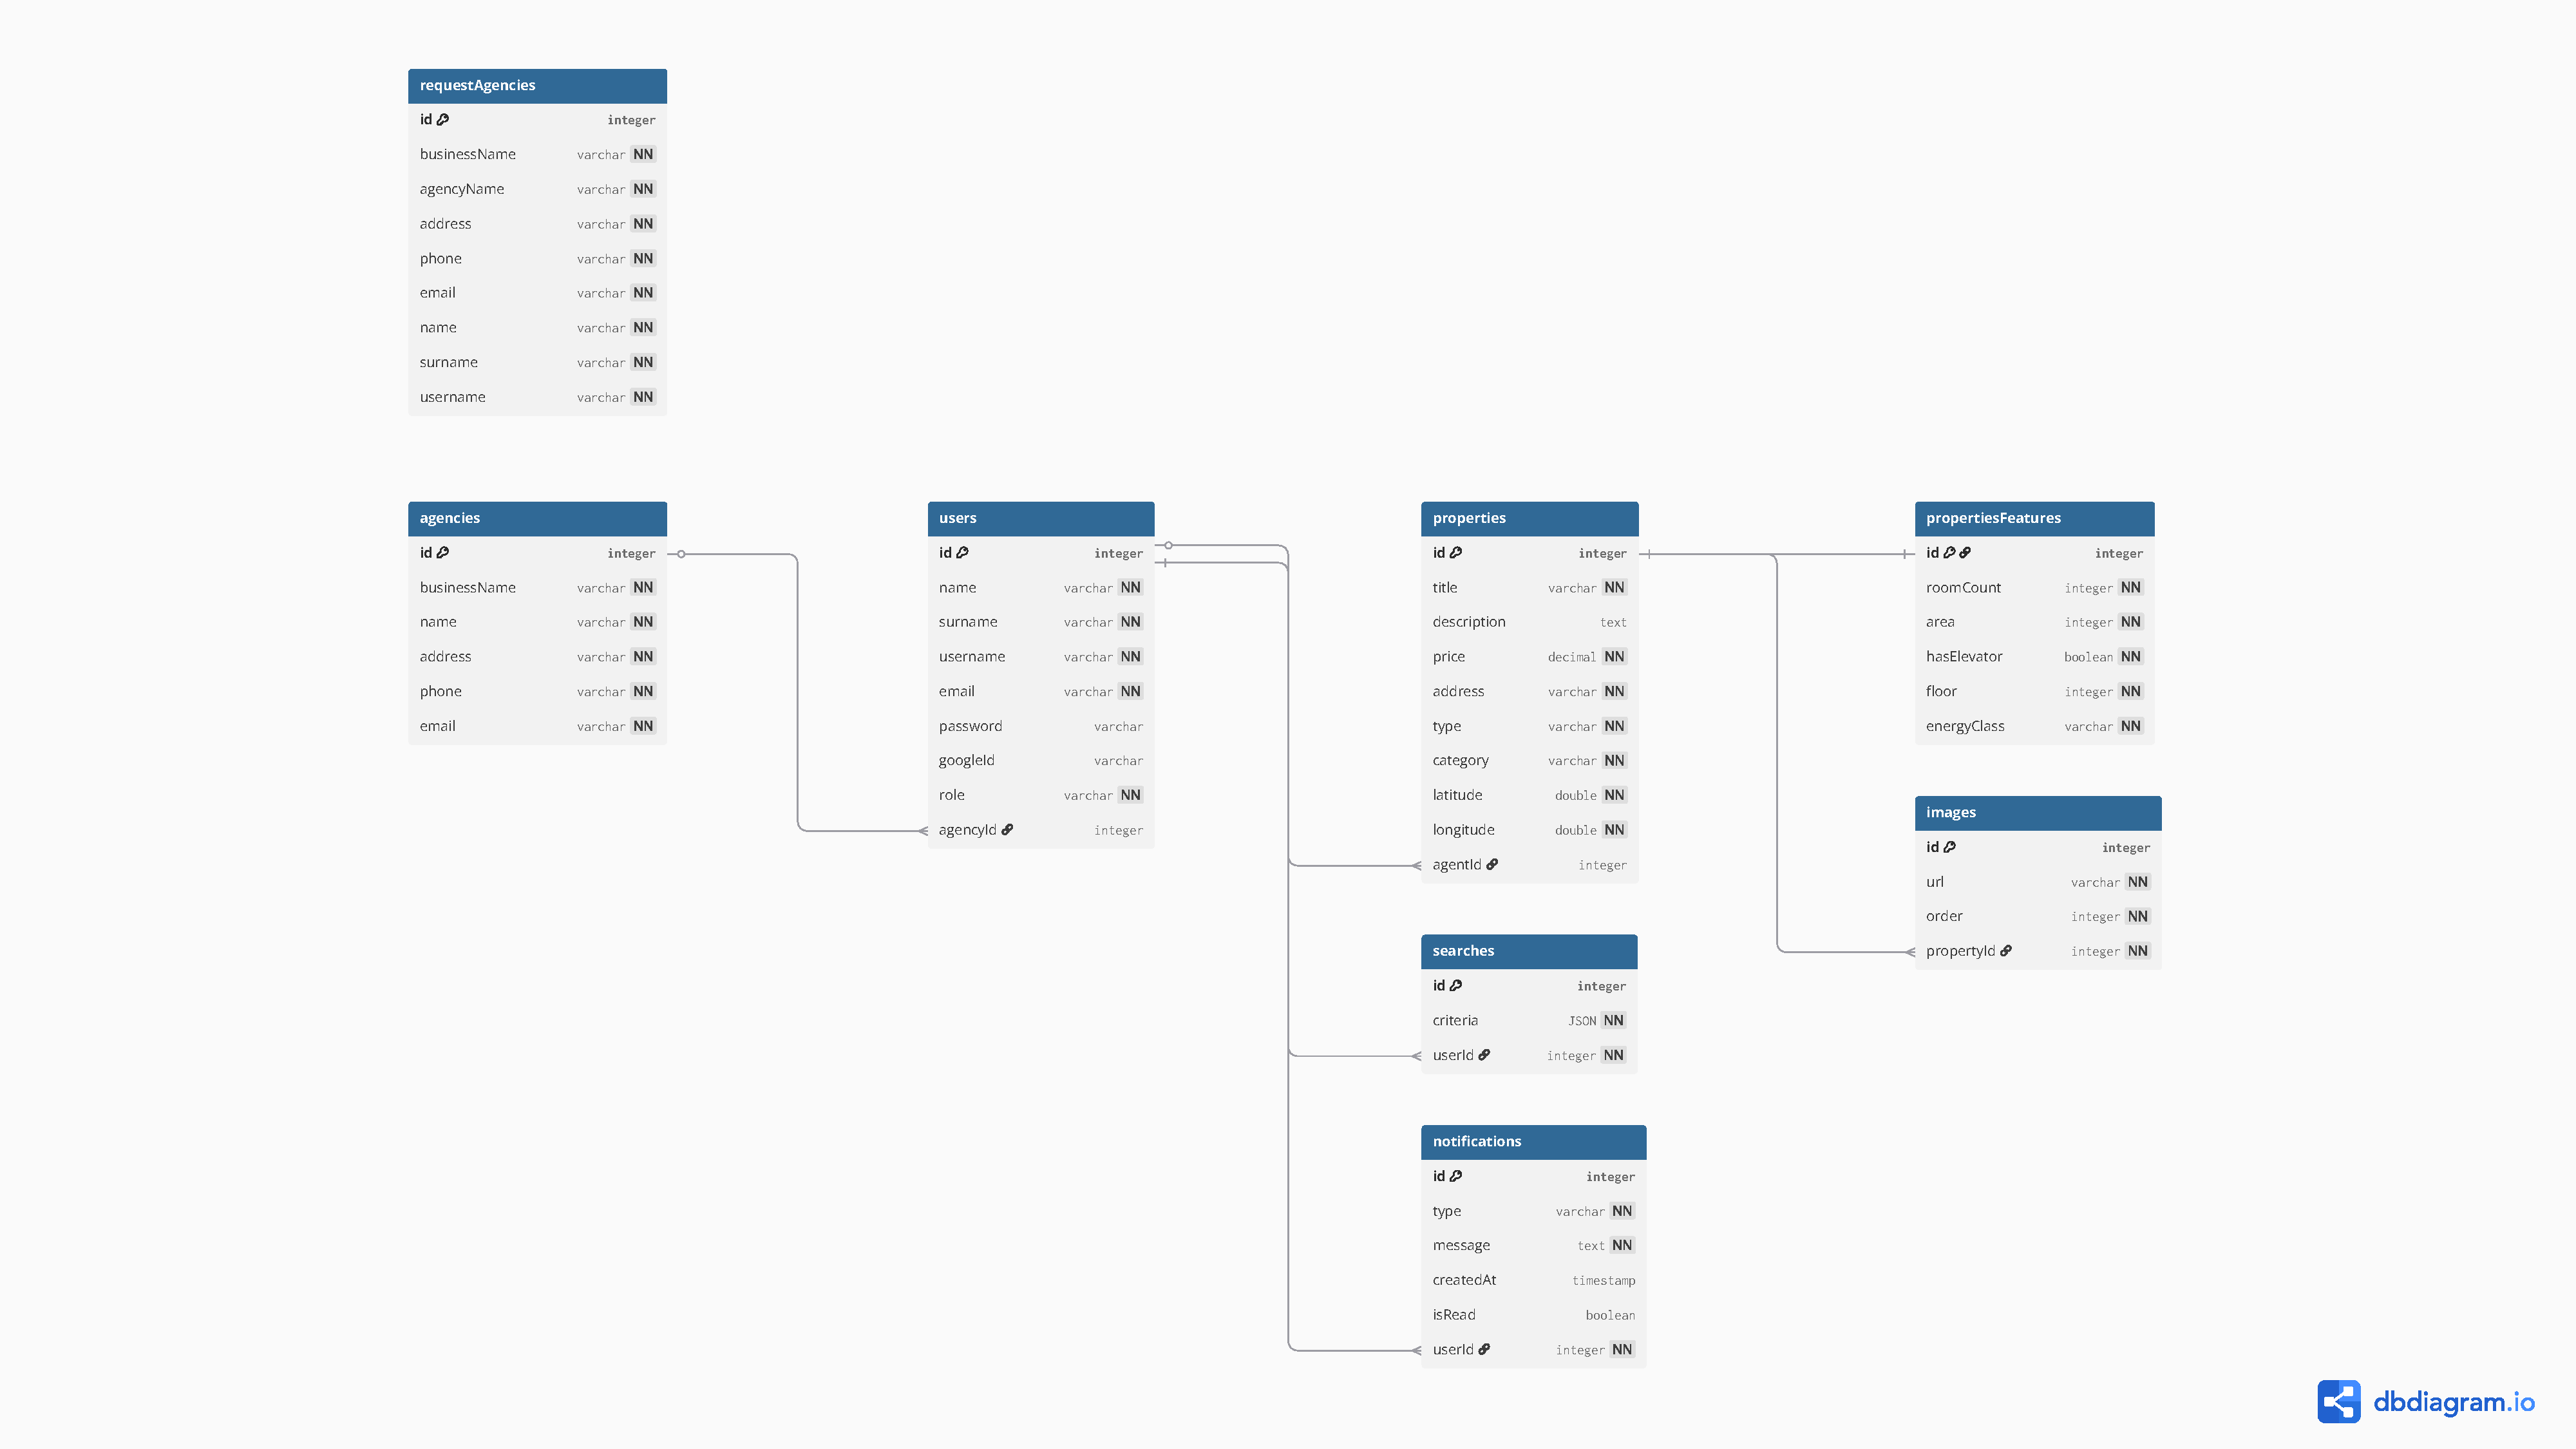
\includepdf[pages=1,scale=0.9,pagecommand={}]{images/DatabaseUML.pdf}
    \label{fig:usecase}
\end{figure}

\newpage

\subsection{Implementazione}

Per la gestione della persistenza dei dati, il sistema si avvale di \textbf{Sequelize}, un \textbf{Object-Relational Mapper} (ORM) per Node.js basato su \textbf{promise}. L'integrazione di Sequelize ha permesso di mappare le classi del dominio applicativo direttamente sulle tabelle del database relazionale, offrendo diversi vantaggi significativi:

\begin{itemize}
    \item \textbf{Astrazione del linguaggio SQL}: Sequelize consente di interagire con la base di dati utilizzando la sintassi JavaScript, eliminando la necessità di scrivere query SQL manuali e riducendo drasticamente il rischio di errori sintattici.
    \item \textbf{Gestione semplificata delle relazioni}: Tramite l'uso di metodi come \texttt{hasMany} e \texttt{belongsTo}, è stato possibile definire in modo programmatico le associazioni tra le entità (es. la relazione tra \texttt{Agencies} e \texttt{Users}), delegando alla libreria la gestione automatica delle chiavi esterne e dei vincoli di integrità.
    \item \textbf{Sincronizzazione e Manutenibilità}: La funzione \texttt{sync()} di Sequelize permette di generare o aggiornare automaticamente lo schema del database partendo dai modelli definiti nel codice, garantendo che la struttura dei dati sia sempre allineata con l'ultima versione dell'applicazione.
    \item \textbf{Sicurezza}: L'ORM fornisce una protezione nativa contro le vulnerabilità di \textbf{SQL Injection}, gestendo in modo sicuro l'escape dei parametri nelle query.
    \item \textbf{Portabilità}: L'astrazione offerta da Sequelize consente di cambiare facilmente il database sottostante (ad esempio, passando da PostgreSQL a MySQL) con minime modifiche al codice, rendendo l'applicazione più flessibile e adattabile a diversi ambienti di produzione.
\end{itemize}

Di seguito viene riportato il codice relativo alla configurazione del database e un esempio di definizione dei modelli principali:

\subsubsection{Creazione del database}
\begin{lstlisting}[language=javascript, caption=Configurazione del database e definizione dei modelli con Sequelize]
import { Sequelize } from "sequelize";
import { createModel as createAgenciesModel } from "./agencies.js";
import { createModel as createUserModel } from "./users.js";
import { createModel as createPropertiesModel } from "./properties.js";
import { createModel as createCaratteristichePropertiesModel } from "./propertiesFeatures.js";
import { createModel as createNotificationsModel } from "./notifications.js";
import { createModel as createSearchesModel } from "./searches.js";
import { createModel as createImagesModel } from "./images.js";
import { createModel as createRequestAgenciesModel } from "./requestAgency.js";

const database = new Sequelize(
  process.env.DB_NAME || 'dietiestates',
  process.env.DB_USER || 'postgres',
  process.env.DB_PASS || 'password',
  {
    host: process.env.DB_HOST || 'localhost',
    dialect: 'postgres',
    retry: { // if connection fails, retry
      match: [/ECONNREFUSED/],
      max: 5
    },
    port: process.env.DB_PORT || 5432,
    logging: false,
  }
);

createUserModel(database);
createAgenciesModel(database);
createPropertiesModel(database);
createCaratteristichePropertiesModel(database);
createNotificationsModel(database);
createSearchesModel(database);
createImagesModel(database);
createRequestAgenciesModel(database);

export const { Users, Agencies, Properties, PropertiesFeatures, Notifications, Searches, Images, RequestAgencies } = database.models;

Agencies.hasMany(Users, { foreignKey: 'agencyId', onDelete: 'CASCADE' });
Users.belongsTo(Agencies, { foreignKey: 'agencyId' });

Users.hasMany(Properties, { foreignKey: 'agentId', onDelete: 'SET NULL' });
Properties.belongsTo(Users, { foreignKey: 'agentId' });

Users.hasMany(Notifications, { foreignKey: 'userId', onDelete: 'CASCADE' });
Notifications.belongsTo(Users, { foreignKey: 'userId' });

Users.hasMany(Searches, { foreignKey: 'userId', onDelete: 'CASCADE' });
Searches.belongsTo(Users, { foreignKey: 'userId' });

PropertiesFeatures.belongsTo(Properties, { foreignKey: 'id', onDelete: 'CASCADE' });
Properties.hasOne(PropertiesFeatures, { foreignKey: 'id', onDelete: 'CASCADE' });

Properties.hasMany(Images, { foreignKey: 'propertyId', allowNull: false, onDelete: 'CASCADE' });
Images.belongsTo(Properties, { foreignKey: 'propertyId' });

export default database;

export async function startConnection() {
  try {
    await database.authenticate();
    await database.sync({ alter: true });
    console.log('Connection has been established successfully.');
  } catch (error) {
    console.error('Unable to connect to the database:', error);
    throw error;
  }
}
\end{lstlisting}

\subsubsection{Creazione di un modello}
\begin{lstlisting}[language=javascript, caption=Creazione del modello "Users" con Sequelize]

import { DataTypes } from 'sequelize';

export function createModel(database){
    database.define('Users', {
        id: {
            type: DataTypes.INTEGER,
            autoIncrement: true,
            primaryKey: true
        },
        name : {
            type: DataTypes.STRING,
            allowNull: false
        },
        surname : {
            type: DataTypes.STRING,
            allowNull: false
        },
        username : {
            type: DataTypes.STRING,
            allowNull: false,
            unique: true
        },
        email : {
            type: DataTypes.STRING,
            allowNull: false,
            unique: true,
        },
        password : {
            type: DataTypes.STRING,
            allowNull: true 
        },
 
        googleId: {
            type: DataTypes.STRING,
            allowNull: true,
            unique: true
        },
        role : {
            type: DataTypes.STRING,
            allowNull: false,
            
        },
        agencyId : {
            type: DataTypes.INTEGER,
            allowNull: true,
            references: {
                model: 'Agencies',
                key: 'id'
            }
        }
    });
}
\end{lstlisting}

\begin{tcolorbox}[colback=gray!10,colframe=black,title=Nota sulla definizione dei modelli]
    Il frammento di codice presentato illustra a titolo esemplificativo la definizione del modello \texttt{Users}. Gli altri modelli presenti nel sistema (come \texttt{Agencies}, \texttt{Properties} o \texttt{Notifications}) seguono una struttura di implementazione analoga: ciascuno viene istanziato tramite il metodo \texttt{database.define}, variando esclusivamente negli attributi specifici e nei vincoli di integrità relativi al proprio dominio funzionale.
\end{tcolorbox}


\newpage

\subsection{Descrizione delle scelte di design dell'interfaccia utente}

\subsubsection{Introduzione}
Abbiamo adottato per la piattaforma di compravendita immobiliare una palette di colori che risponde a precise necessità psicologiche: la generazione di fiducia, il richiamo alla solidità materica e la massimizzazione dei tassi di conversione attraverso il contrasto visivo.

\subsubsection{Visualizzazione della Palette}

Di seguito sono riportati i codici colore principali che compongono l'identità visiva:

\begin{center}
    \begin{minipage}{0.3\textwidth}
        \begin{tcolorbox}[colback=DeepNavy, colframe=black!10, height=3cm, title=\textcolor{DeepEarth}{Deep Navy}, center title]
            \vfill \centering \color{white} \#173857
        \end{tcolorbox}
    \end{minipage}
    \begin{minipage}{0.3\textwidth}
        \begin{tcolorbox}[colback=SteelBlue, colframe=black!10, height=3cm, title=\textcolor{DeepEarth}{Steel Blue}, center title]
            \vfill \centering \color{white} \#4D7396
        \end{tcolorbox}
    \end{minipage}
    \begin{minipage}{0.3\textwidth}
        \begin{tcolorbox}[colback=DeepEarth, colframe=black!10, height=3cm, title=\textcolor{DeepEarth}{Deep Earth}, center title]
            \vfill \centering \color{white} \#573E17
        \end{tcolorbox}
    \end{minipage}

    \vspace{0.5cm}

    \begin{minipage}{0.3\textwidth}
        \begin{tcolorbox}[colback=SandGold, colframe=black!10, height=3cm, title=\textcolor{DeepEarth}{Sand Gold}, center title]
            \vfill \centering \color{white} \#AC9166
        \end{tcolorbox}
    \end{minipage}
    \begin{minipage}{0.3\textwidth}
        \begin{tcolorbox}[colback=WarmCream, colframe=black!10, height=3cm, title=\textcolor{DeepEarth}{Warm Cream}, center title]
            \vfill \centering \color{DeepEarth} \#FFF3DF
        \end{tcolorbox}
    \end{minipage}
    \begin{minipage}{0.3\textwidth}
        \begin{tcolorbox}[colback=AccentOrange, colframe=black!10, height=3cm, title=\textcolor{DeepEarth}{Accent Color}, center title]
            \vfill \centering \color{white} \#F39C12
        \end{tcolorbox}
    \end{minipage}
\end{center}

\subsubsection{Il Pilastro della Fiducia: Deep Navy (\#173857)}
Il colore dominante della composizione è il \textbf{Deep Navy}. In un mercato dove l'investimento del cliente è massivo, il blu scuro funge da ancora psicologica.
\begin{itemize}
    \item \textbf{Istituzionalità:} Comunica che l'agenzia non è solo un intermediario, ma un'istituzione solida.
    \item \textbf{Serietà Finanziaria:} È il colore associato globalmente ai servizi bancari e legali, essenziali nella fase di rogito e mutuo.
    \item \textbf{Leggibilità:} Utilizzato per gli header e la tipografia principale, garantisce un'esperienza utente riposante e autorevole.
\end{itemize}

\subsubsection{Elementi Materici e Accoglienza}
Mentre il blu stabilisce la professionalità, i toni terra (\textbf{\#573E17} e \textbf{\#AC9166}) introducono il concetto di ``Casa''.
\begin{itemize}
    \item \textbf{Richiamo Naturale:} Questi colori evocano materiali nobili come il legno di rovere, il cuoio e la pietra.
    \item \textbf{Comfort Domestico:} Il \textbf{Warm Cream (\#FFF3DF)}, utilizzato per gli sfondi delle schede o delle sezioni, sostituisce il bianco puro per eliminare il senso di freddezza, creando un ambiente digitale accogliente.
\end{itemize}

\subsubsection{Il Trigger di Conversione: Arancione Ambra (\#F39C12)}
L'elemento di forza della strategia è l'uso di piccoli ma intensi punti di contrasto in \textbf{Arancione Ambra}. Questo colore è posizionato strategicamente al di fuori dell'armonia principale per creare un'interruzione visiva.

\begin{tcolorbox}[colback=AccentOrange!10, colframe=AccentOrange, title=Logica della Call to Action (CTA)]
    L'arancione è il colore complementare dinamico dei toni bluastri. Quando l'utente scorre una lista di immobili (dominata dai blu e dai marroni), l'occhio viene naturalmente attratto dai pulsanti \textit{``Cerca''} o \textit{``Prezzo''} colorati con \#F39C12. Questo riduce il carico cognitivo e accelera la decisione d'acquisto.
\end{tcolorbox}

\subsubsection{Conclusioni}
L'equilibrio tra la freddezza autorevole del blu e il calore organico dei toni sabbia crea un'immagine di marca premium. L'integrazione dell'arancione come elemento di contrasto puro garantisce che il sito non sia solo una vetrina elegante, ma una macchina da conversione efficiente.

\newpage

\subsection{Diagramma delle Classi}

Il design del sistema è stato guidato dai principi di \textbf{modularità} e \textbf{Separation of Concerns} (Separazione degli Interessi), con l'obiettivo di massimizzare la manutenibilità e la testabilità del codice. L'architettura adotta il pattern \textbf{MVC} (Model-View-Controller) e si fonda su due pilastri fondamentali della progettazione orientata agli oggetti:

\begin{itemize}
    \item \textbf{Single Responsibility Principle (SRP)}: Ogni classe e modulo è progettato per avere un'unica responsabilità ben definita. Questo riduce la complessità interna e facilita l'individuazione di bug o la modifica di funzionalità specifiche senza impatti imprevisti sul resto del sistema.
    \item \textbf{Basso Accoppiamento (Low Coupling)}: Le interazioni tra i diversi layer avvengono tramite interfacce chiare (metodi statici dei controller), riducendo le dipendenze dirette tra componenti distanti. Ciò permette, ad esempio, di modificare la logica di business senza dover alterare la struttura delle rotte o la configurazione del database.
\end{itemize}

\subsubsection{Organizzazione a Livelli e Responsabilità}
La scomposizione in classi segue una stratificazione logica dove ogni livello rispetta rigorosamente il principio della singola responsabilità:

\begin{itemize}
    \item \textbf{Routing Layer (Rotte)}: Gestisce esclusivamente l'interfaccia con il protocollo HTTP. La sua unica responsabilità è mappare gli endpoint alle funzioni dei controller e orchestrare la catena di middleware (autenticazione, autorizzazione e validazione). Questo layer non contiene logica di business, garantendo un \textit{disaccoppiamento} totale tra l'endpoint e l'implementazione della funzione.

    \item \textbf{Controller Layer (Logica di Business)}: Costituisce il cuore operativo. La sua responsabilità è l'orchestrazione dei dati e l'applicazione delle regole di business. Grazie al basso accoppiamento, i controller rimangono agnostici rispetto al trasporto (HTTP) e si interfacciano con il database esclusivamente tramite i modelli, facilitando la scrittura di \textbf{Unit Test} isolati.

    \item \textbf{Model Layer (Persistenza)}: Ha l'unica responsabilità di definire la struttura dei dati e le relazioni tra le entità tramite l'ORM Sequelize. Centralizzando la definizione dello schema e dei vincoli di integrità, si assicura che la validità dei dati sia garantita in modo uniforme in tutta l'applicazione.
\end{itemize}

\vspace{0.25cm} % Spaziatura verticale
\noindent % Disabilita l'indentazione del nuovo paragrafo
\begin{tcolorbox}[colback=gray!10,colframe=black,title=Nota schema UML]
    Alcuni modelli sono stati raggruppati insieme ad altri siccome il loro accoppiamento serve per riflettere le dipendenze funzionali strette e l'uso di modelli di dati condivisi, garantendo una visione d'insieme più aderente alla logica del codice. Questa scelta progettuale permette di ridurre la complessità visiva dello schema, evidenziando come i controller collaborino per operare sugli stessi set di dati fondamentali.
\end{tcolorbox}

\subsubsection{Diagramma UML del modulo "Auth \& User"}
\begin{figure}[H]
    \centering
    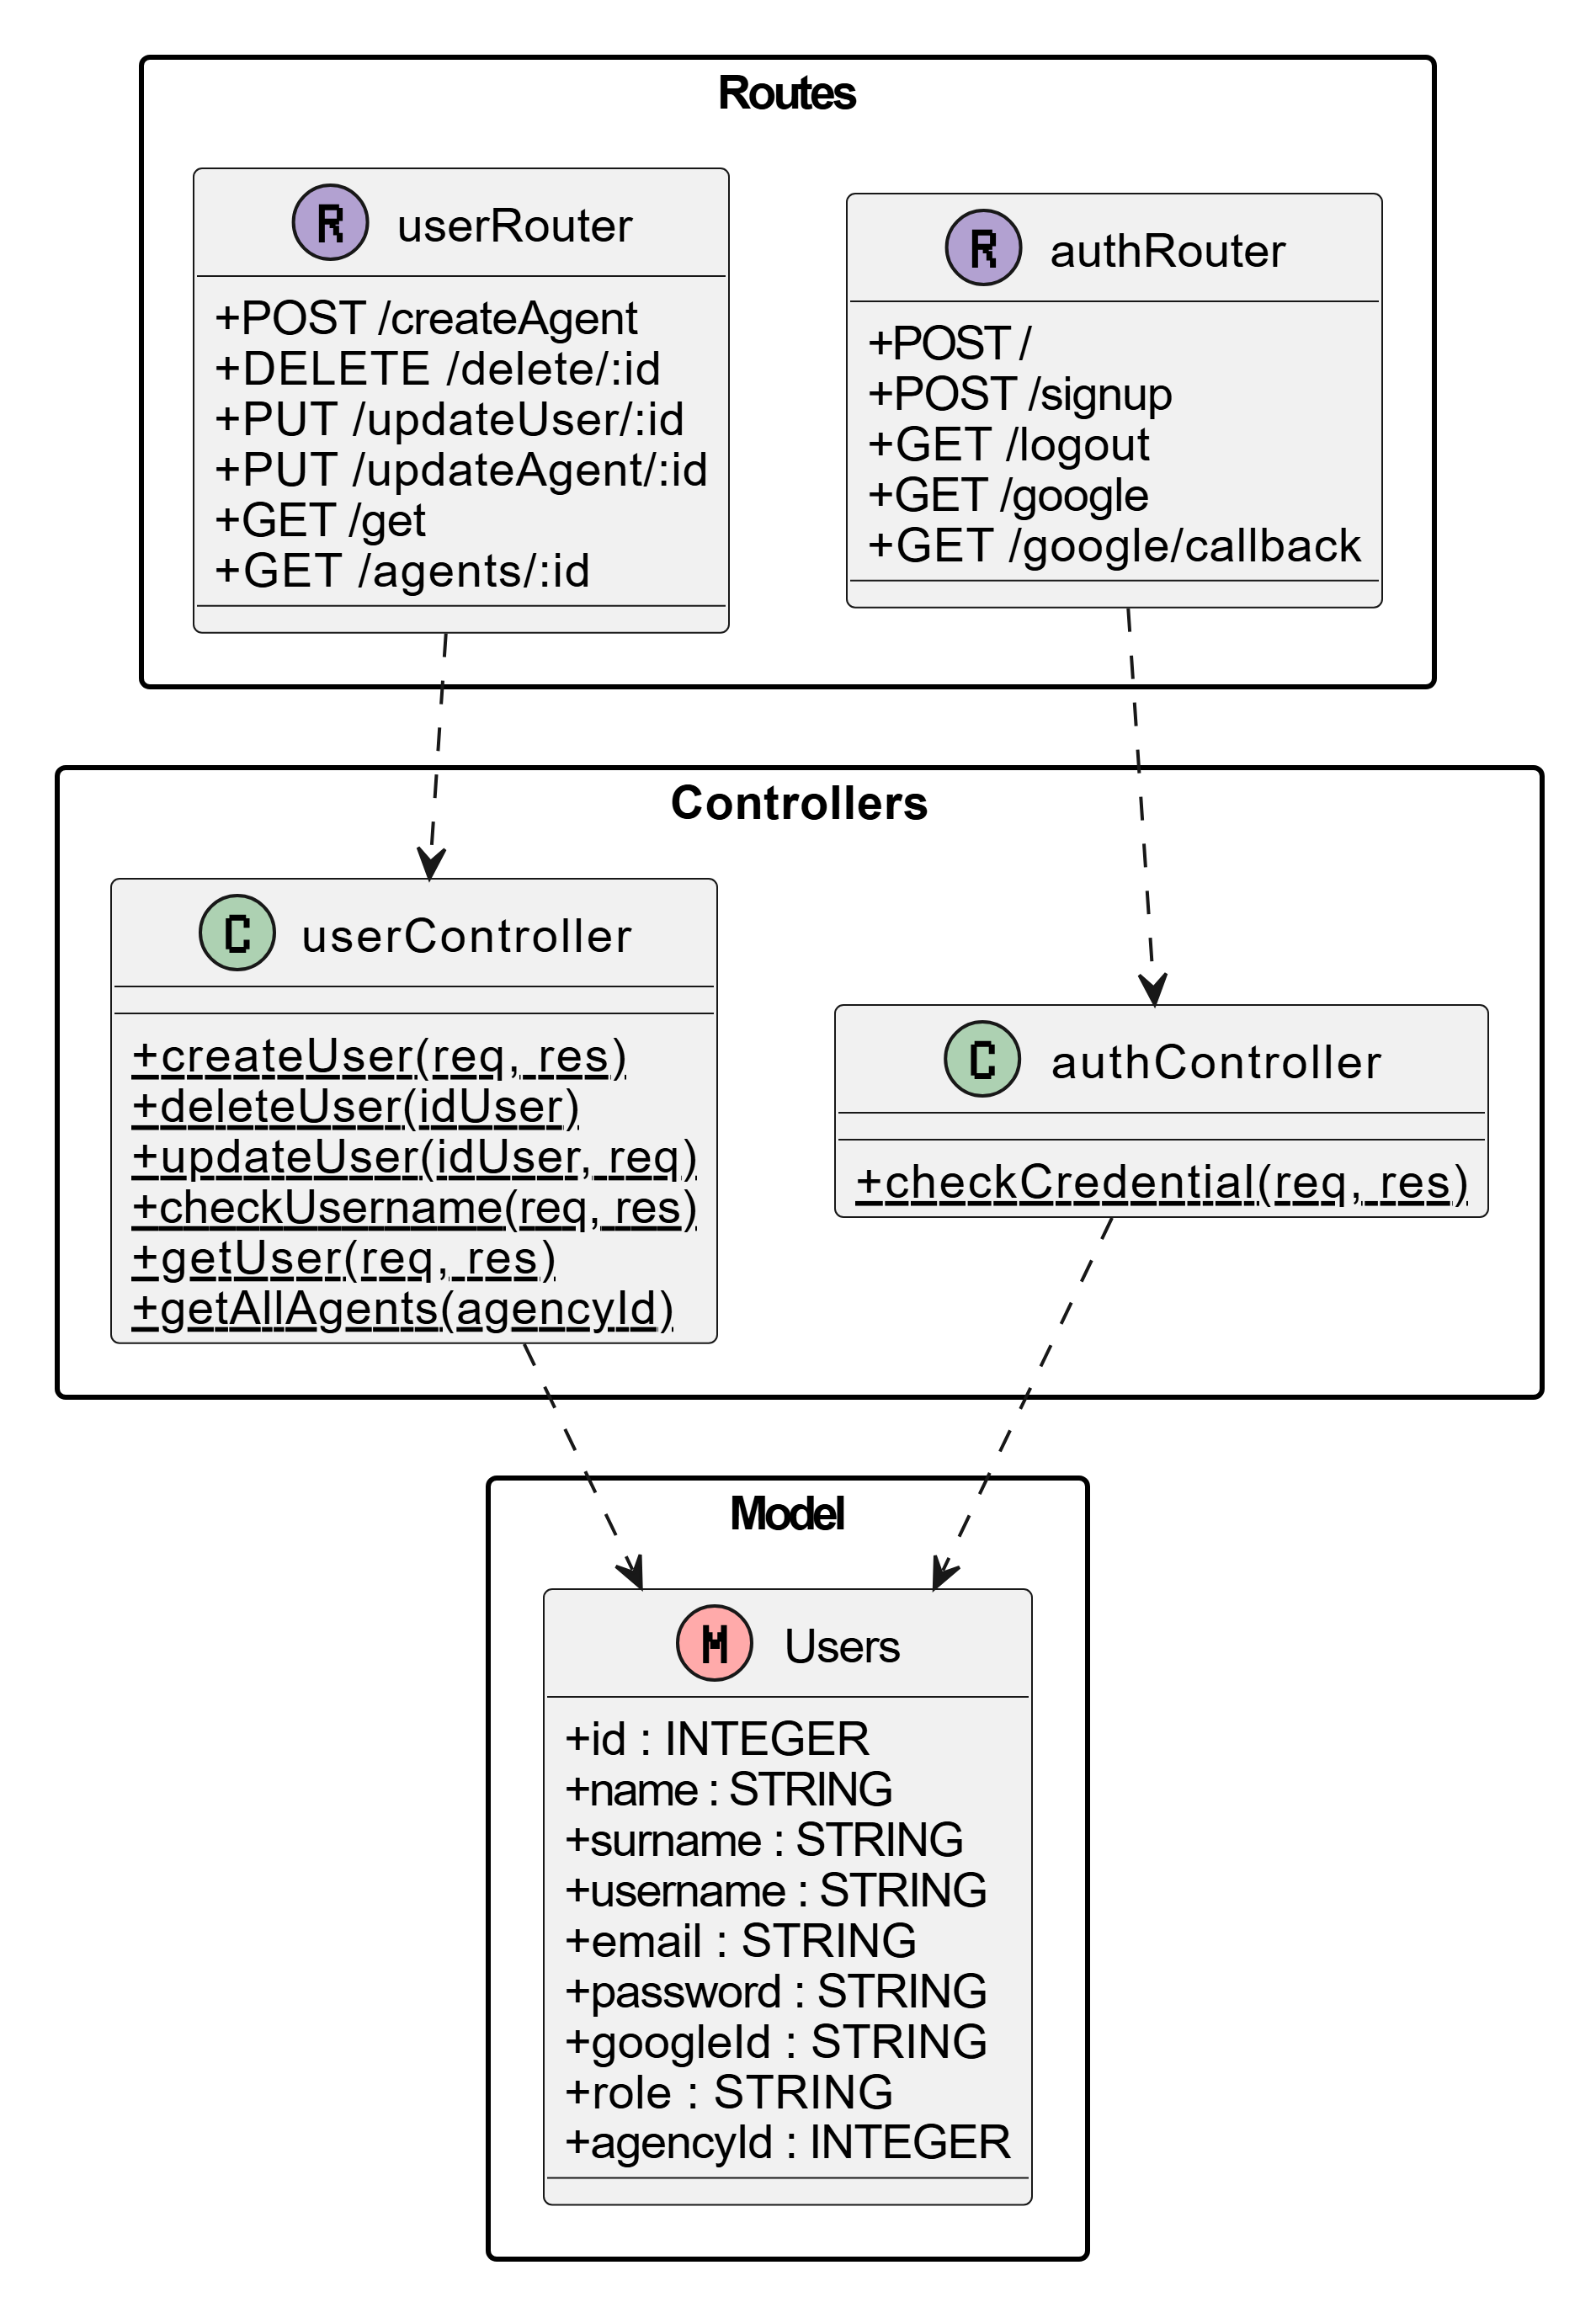
\includegraphics[width=0.8\textwidth]{images/fotoUML/UserAuthUML.png}
    \caption{Schema UML Auth e User}
\end{figure}

\newpage
\subsubsection{Diagramma UML del modulo "Properties \& Images"}
\begin{figure}[H]
    \centering
    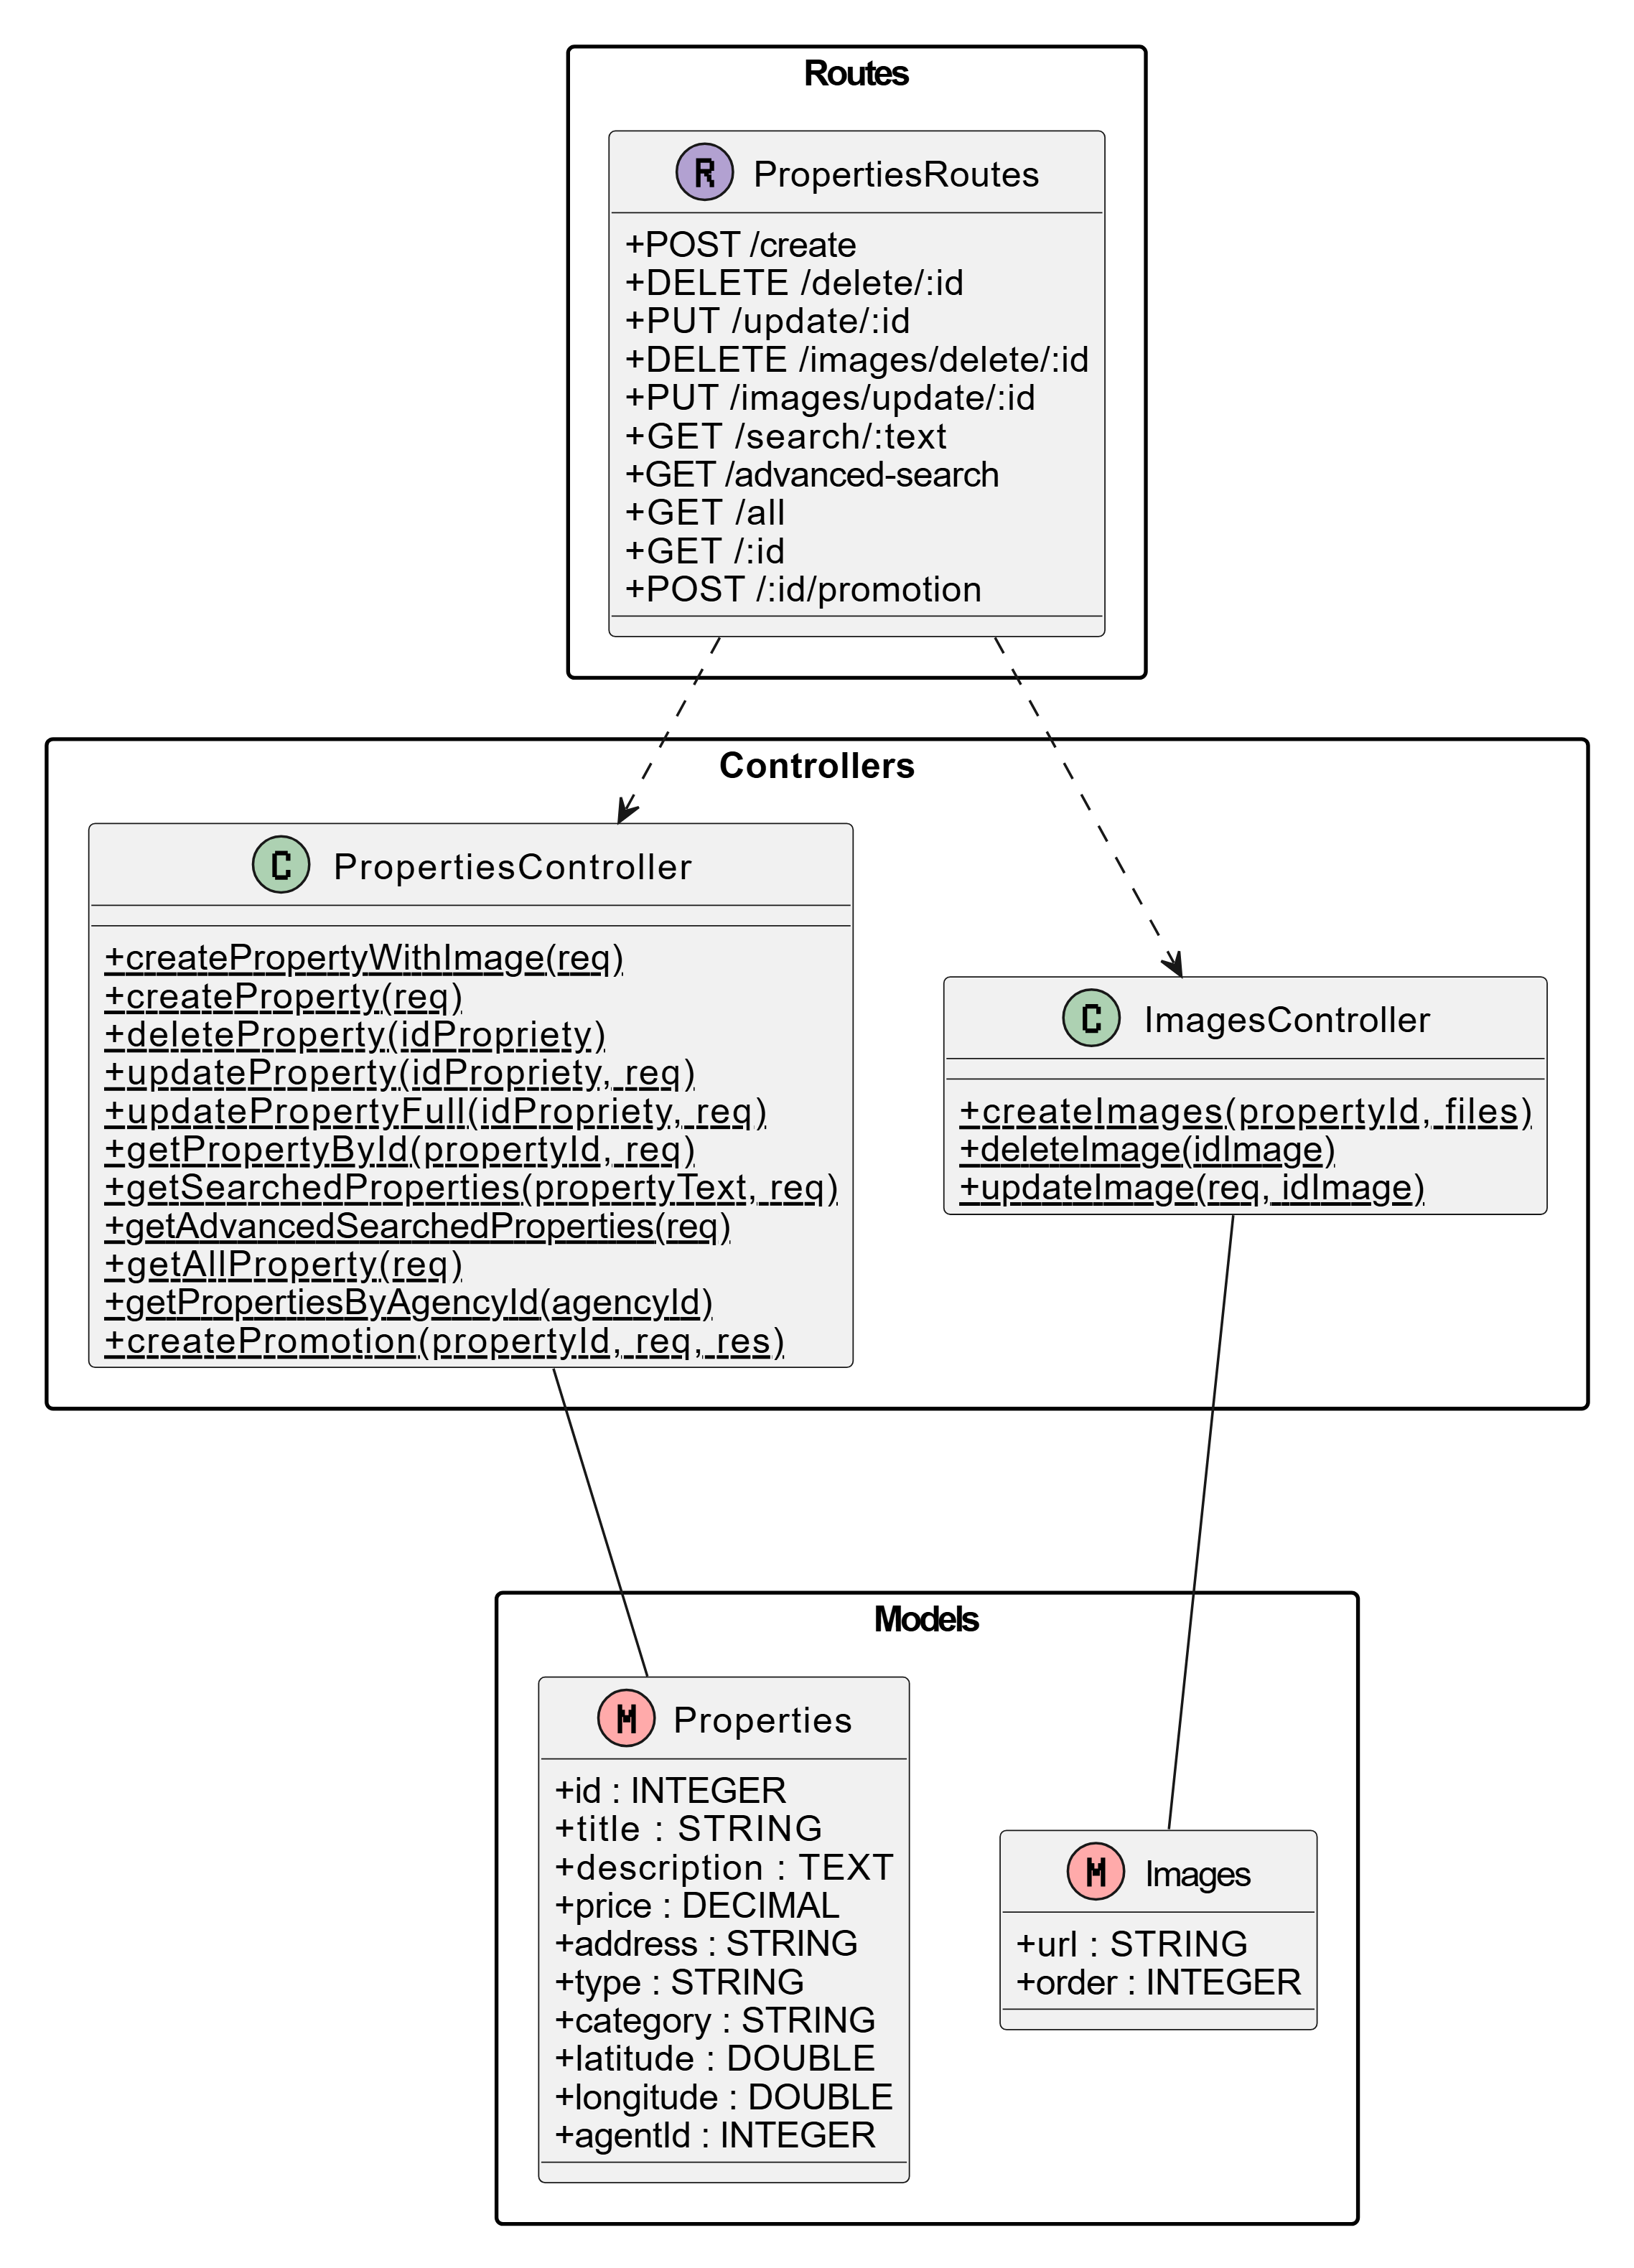
\includegraphics[width=0.8\textwidth]{images/fotoUML/PropertiesImagesUML.png}
    \caption{Schema UML Properties e Images}
\end{figure}
\newpage

\subsubsection{Diagramma UML del modello "PropertiesFeatures"}
\begin{figure}[H]
    \centering
    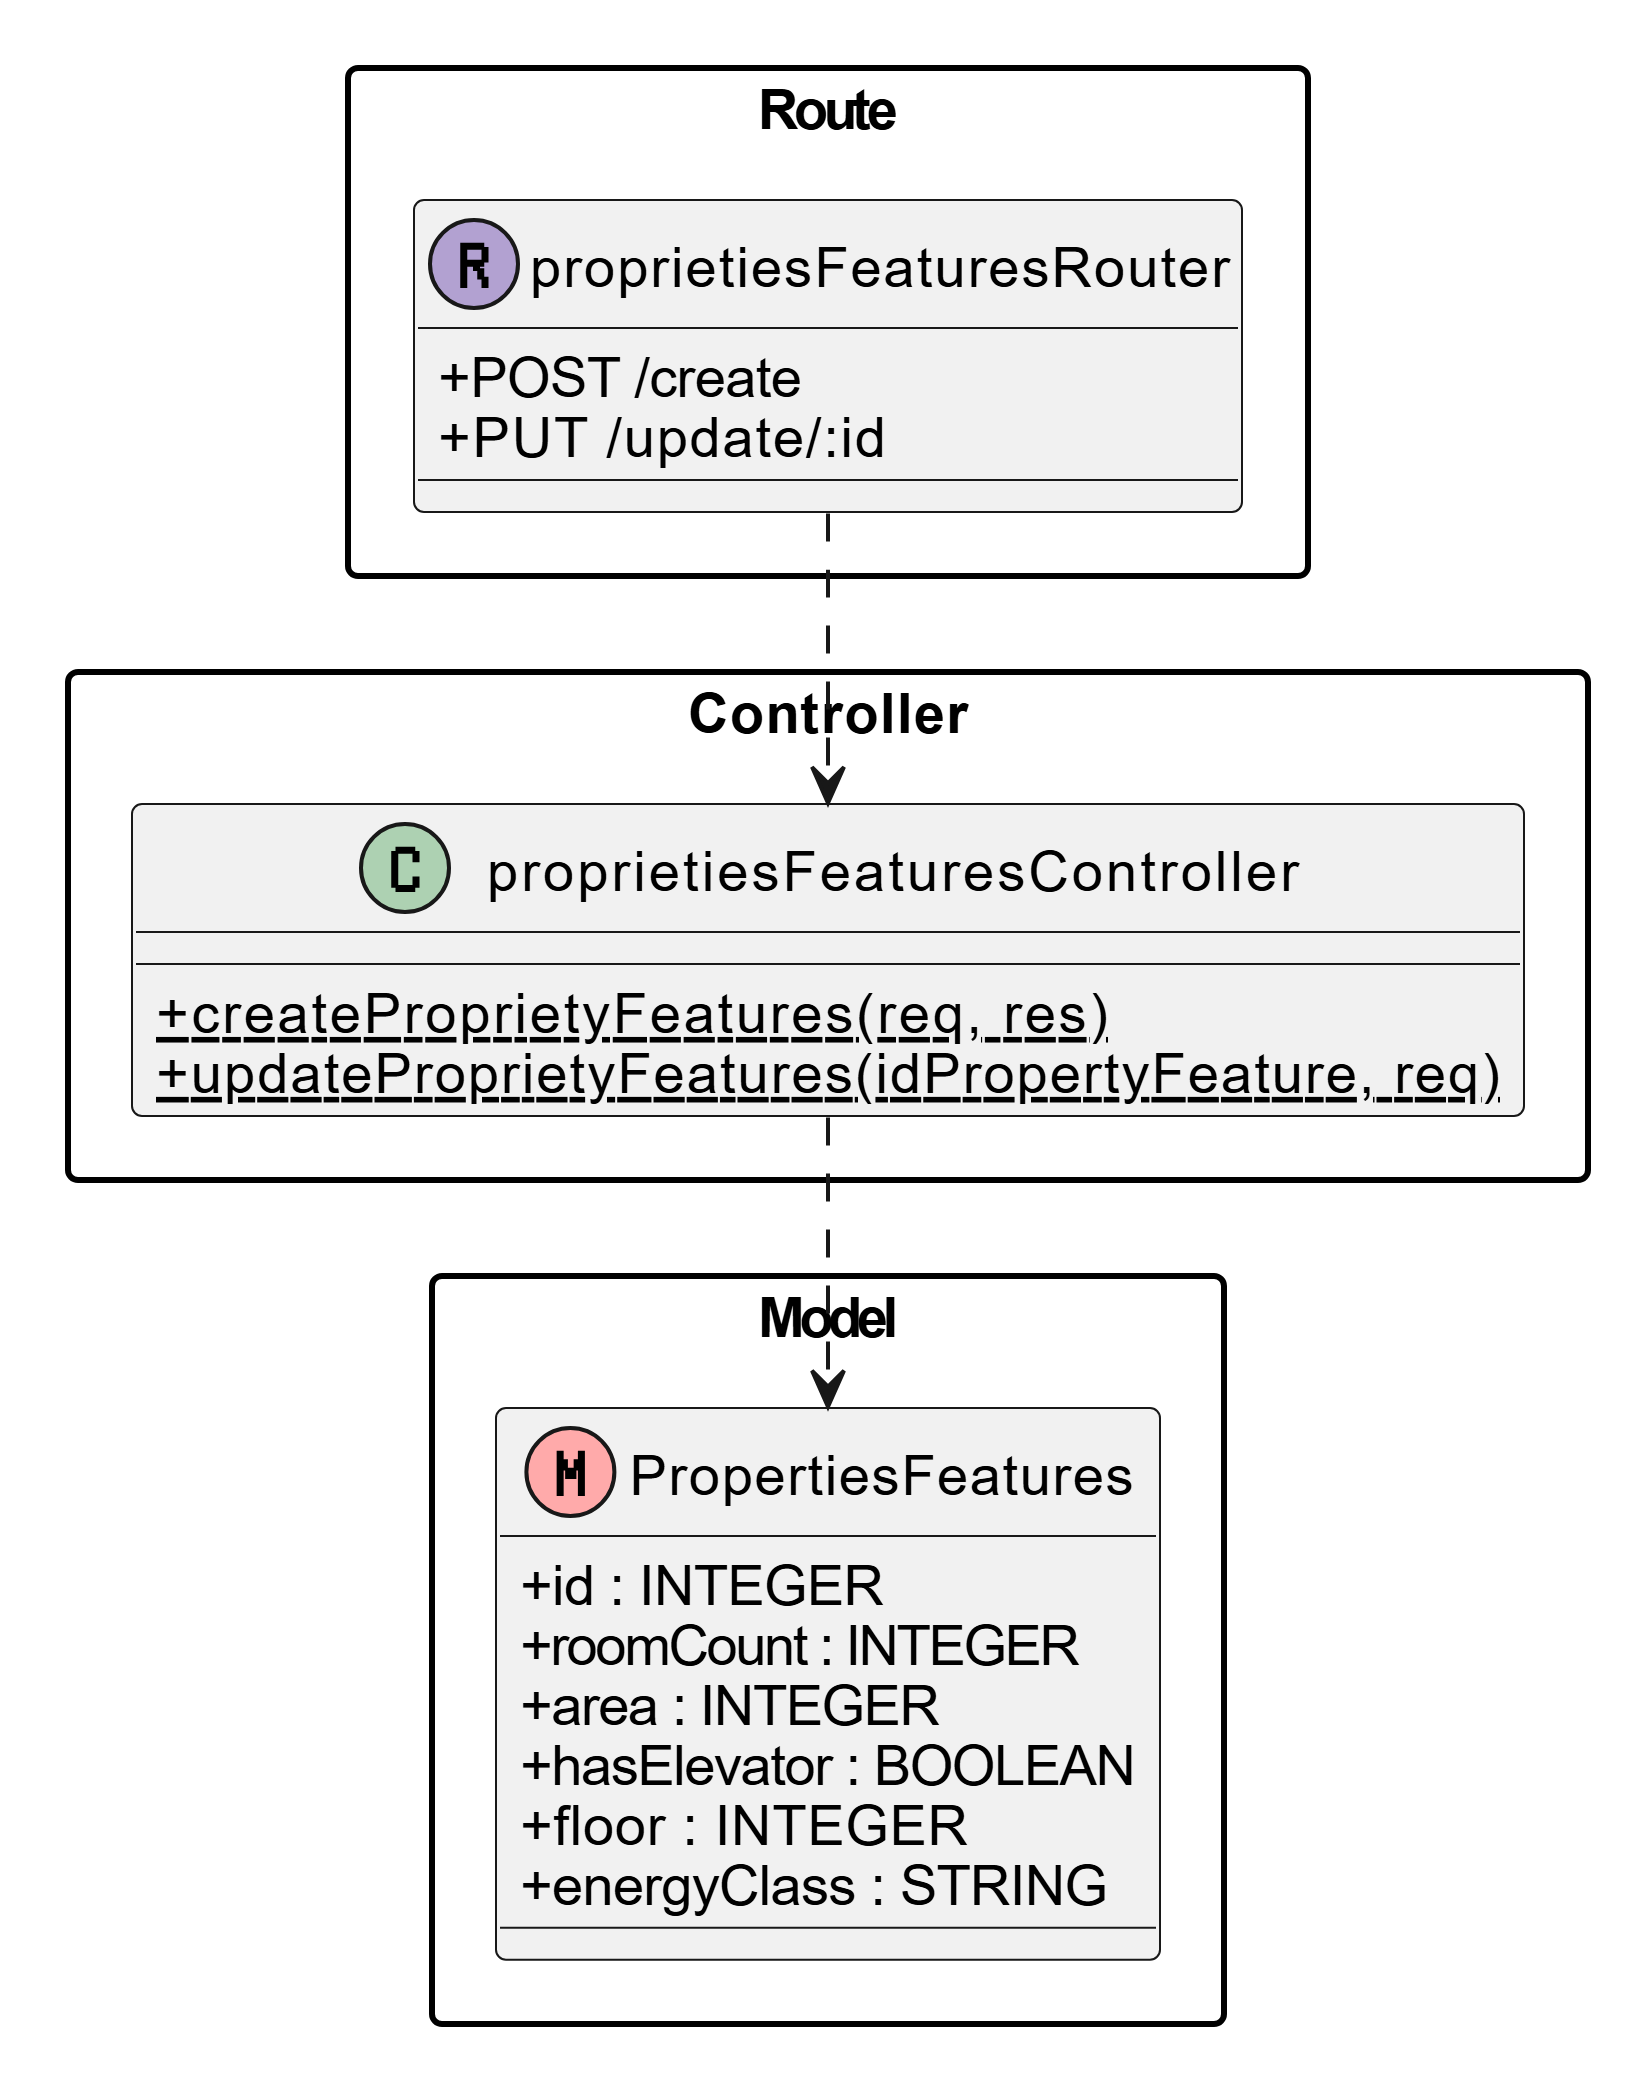
\includegraphics[width=0.6\textwidth]{images/fotoUML/PropertiesFeaturesUML.png}
    \caption{Schema UML PropertiesFeatures}
\end{figure}
\newpage

\subsubsection{Diagramma UML del modello "Agencies"}
\begin{figure}[H]
    \centering
    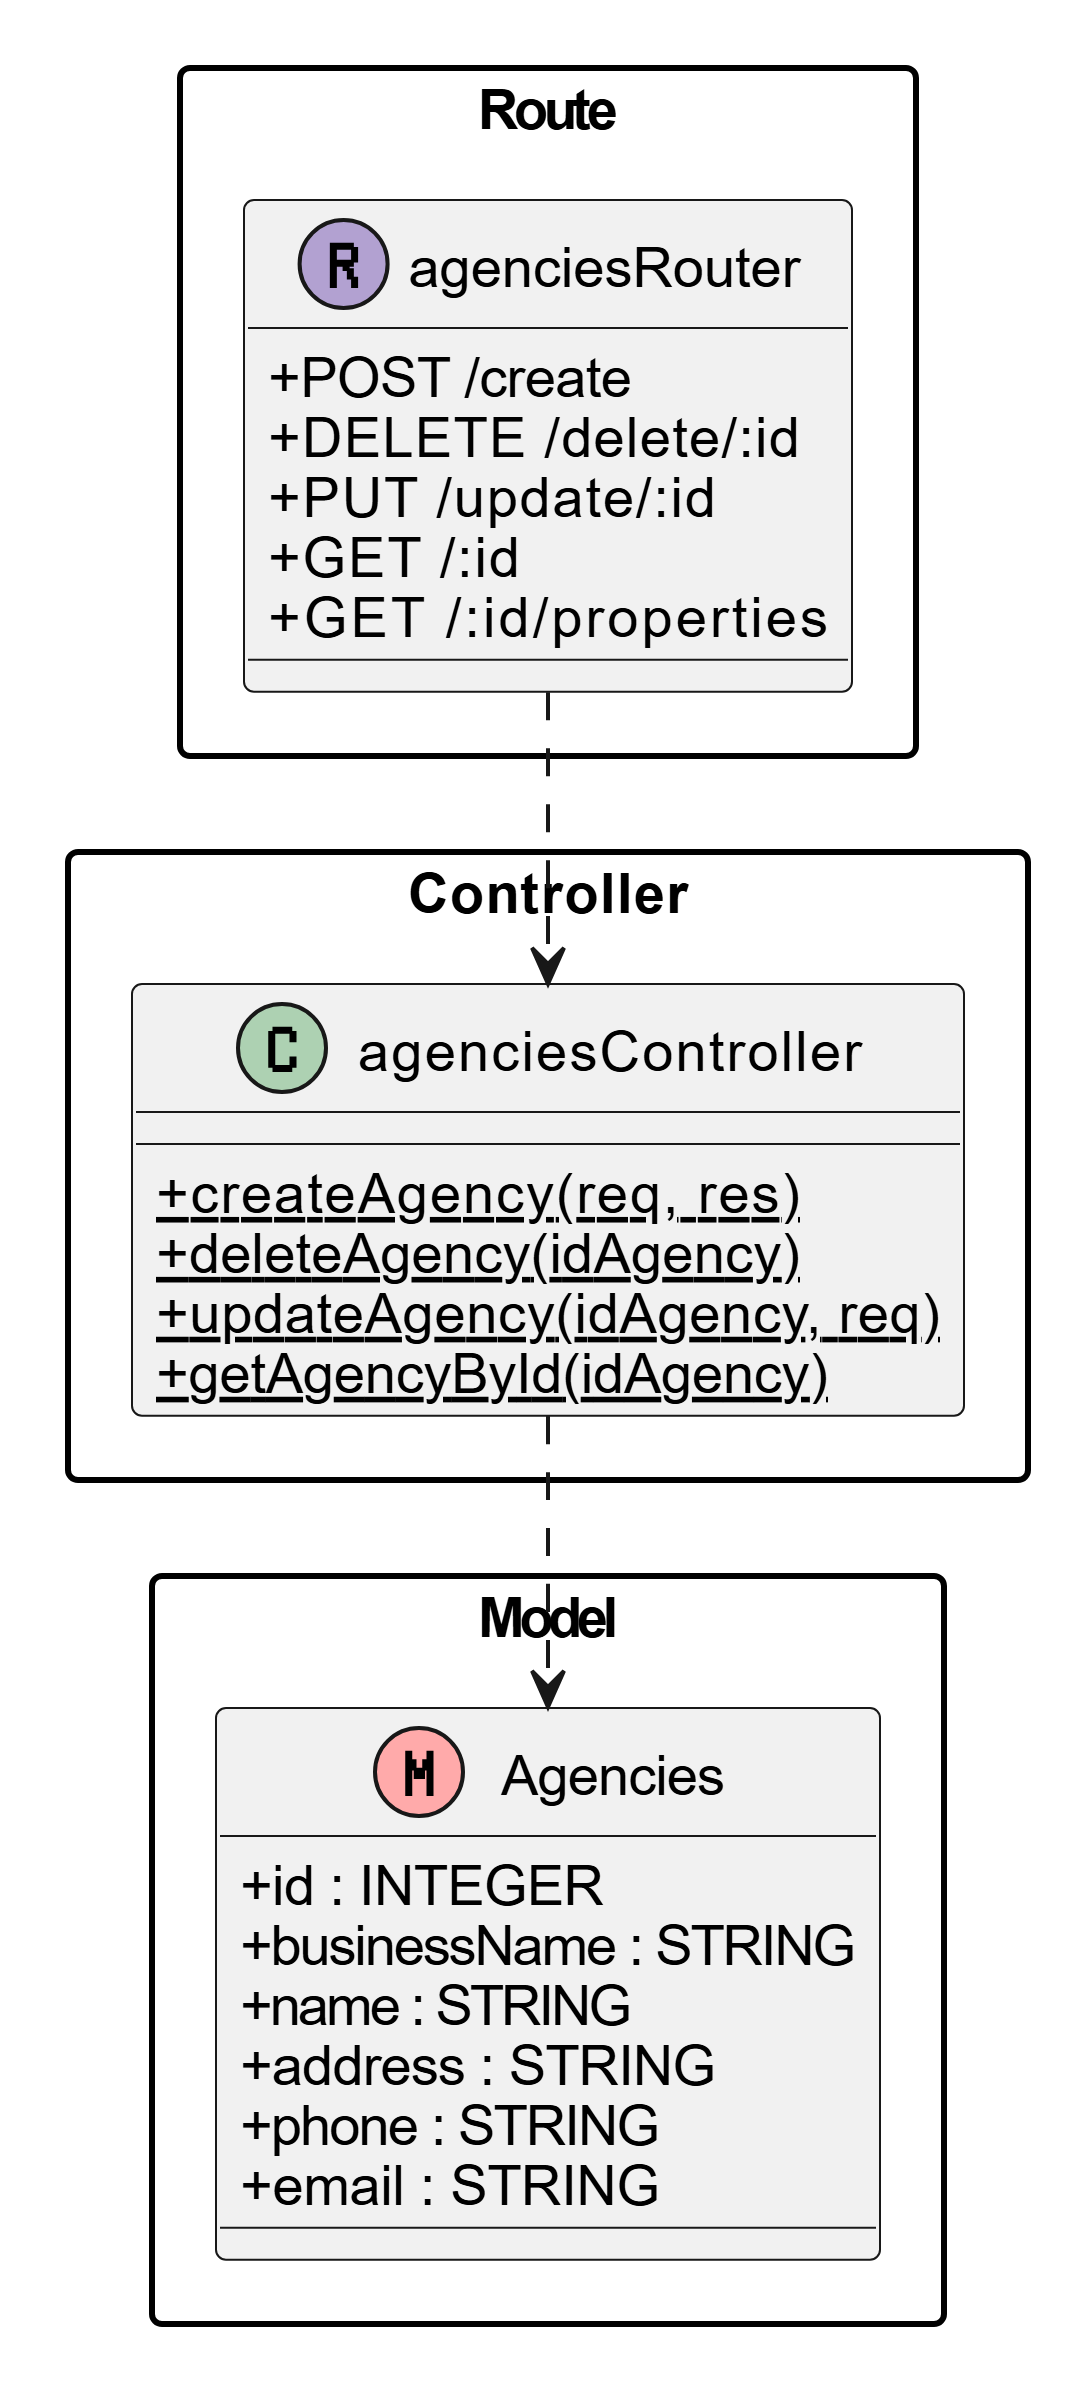
\includegraphics[width=0.5\textwidth]{images/fotoUML/AgenciesUML.png}
    \caption{Schema UML Agencies}
\end{figure}
\newpage

\subsubsection{Diagramma UML del modello "RequestAgencies"}
\begin{figure}[H]
    \centering
    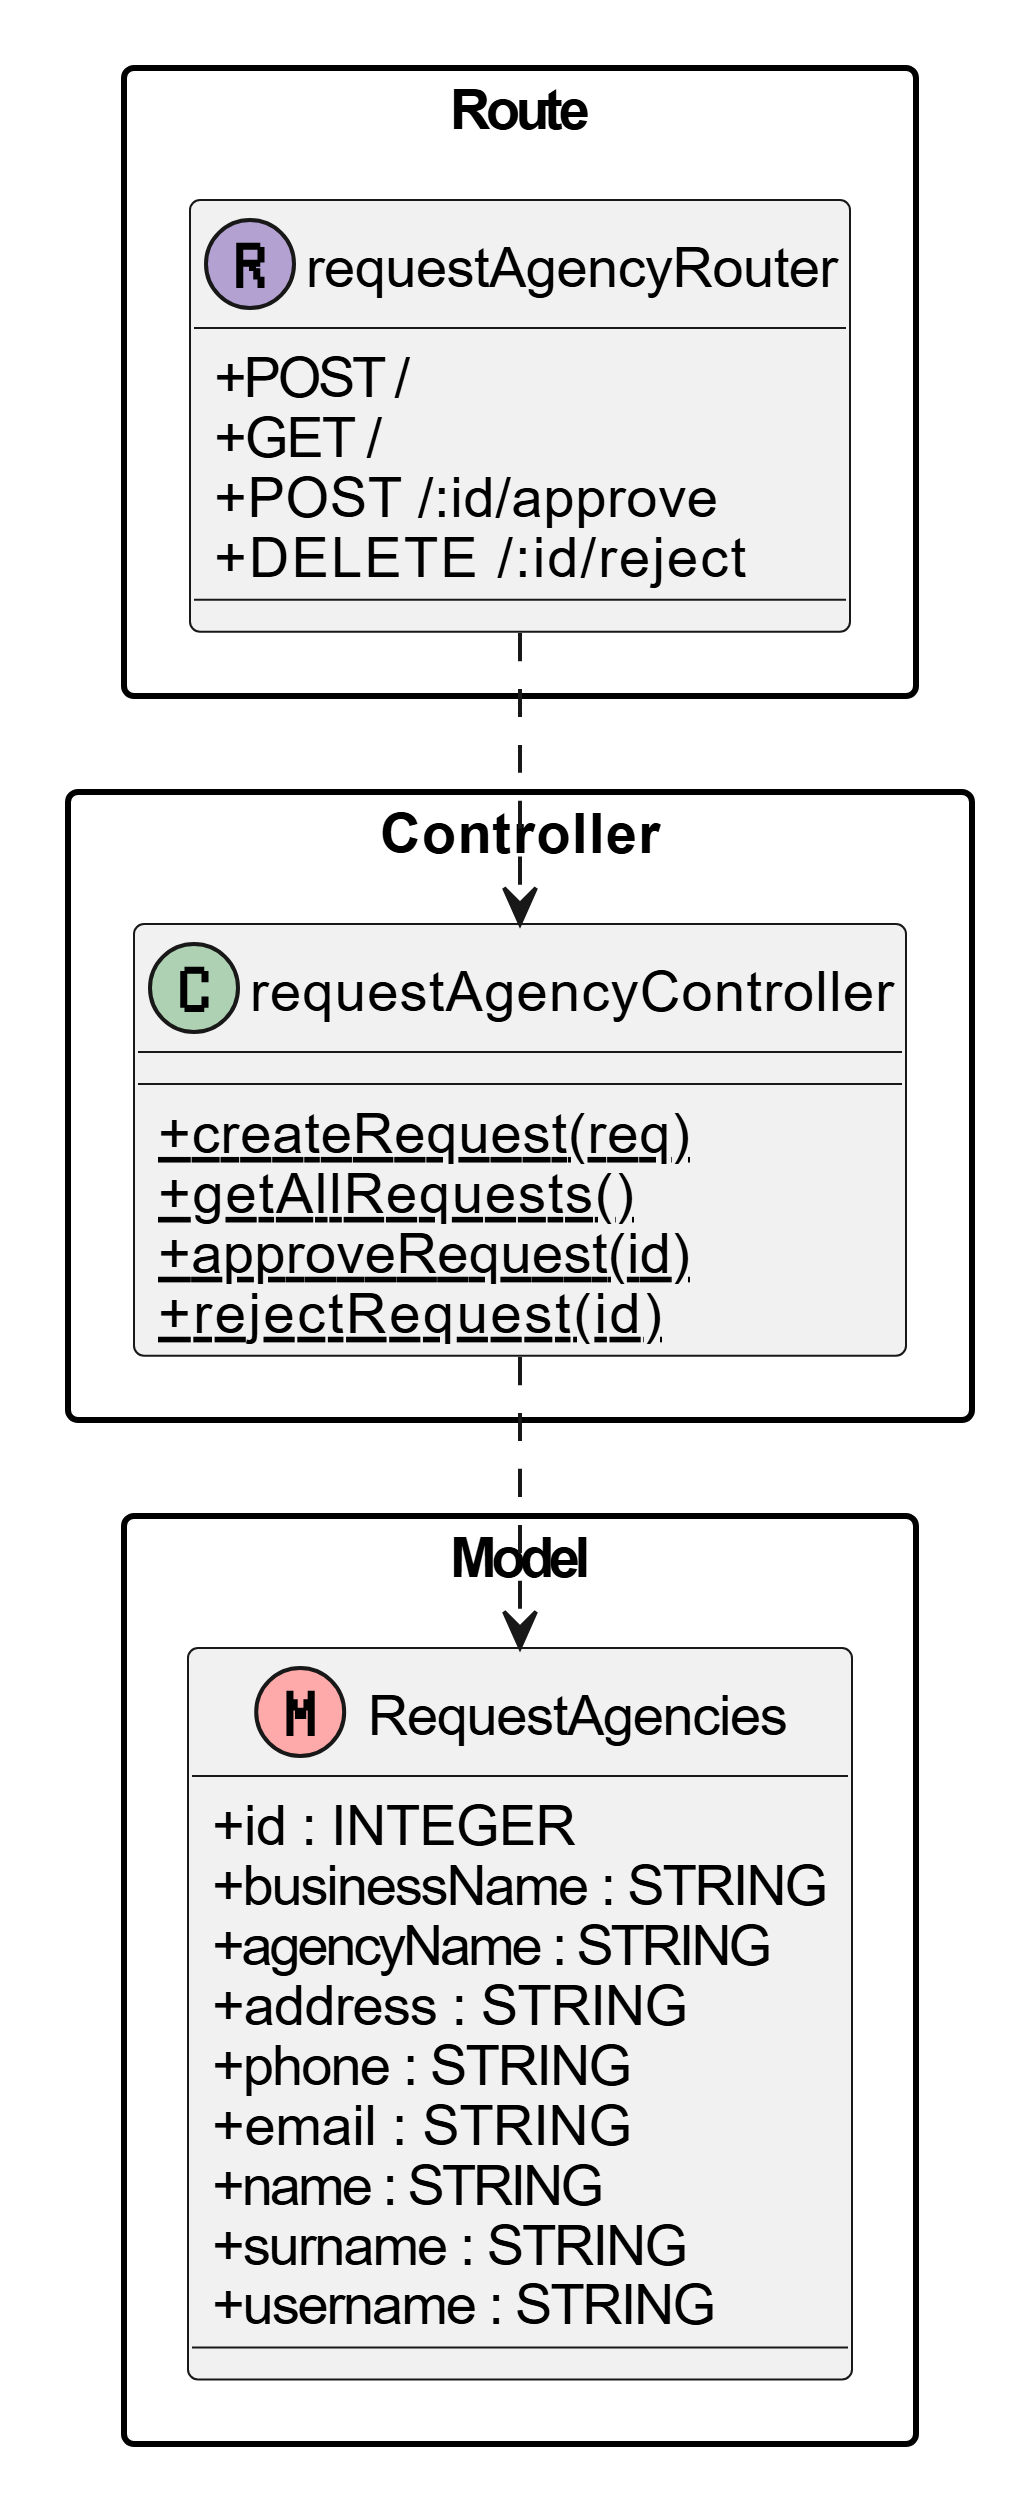
\includegraphics[width=0.5\textwidth]{images/fotoUML/RequestAgenciesUML.png}
    \caption{Schema UML RequestAgencies}
\end{figure}
\newpage

\subsubsection{Diagramma UML del modello "Notifications"}
\begin{figure}[H]
    \centering
    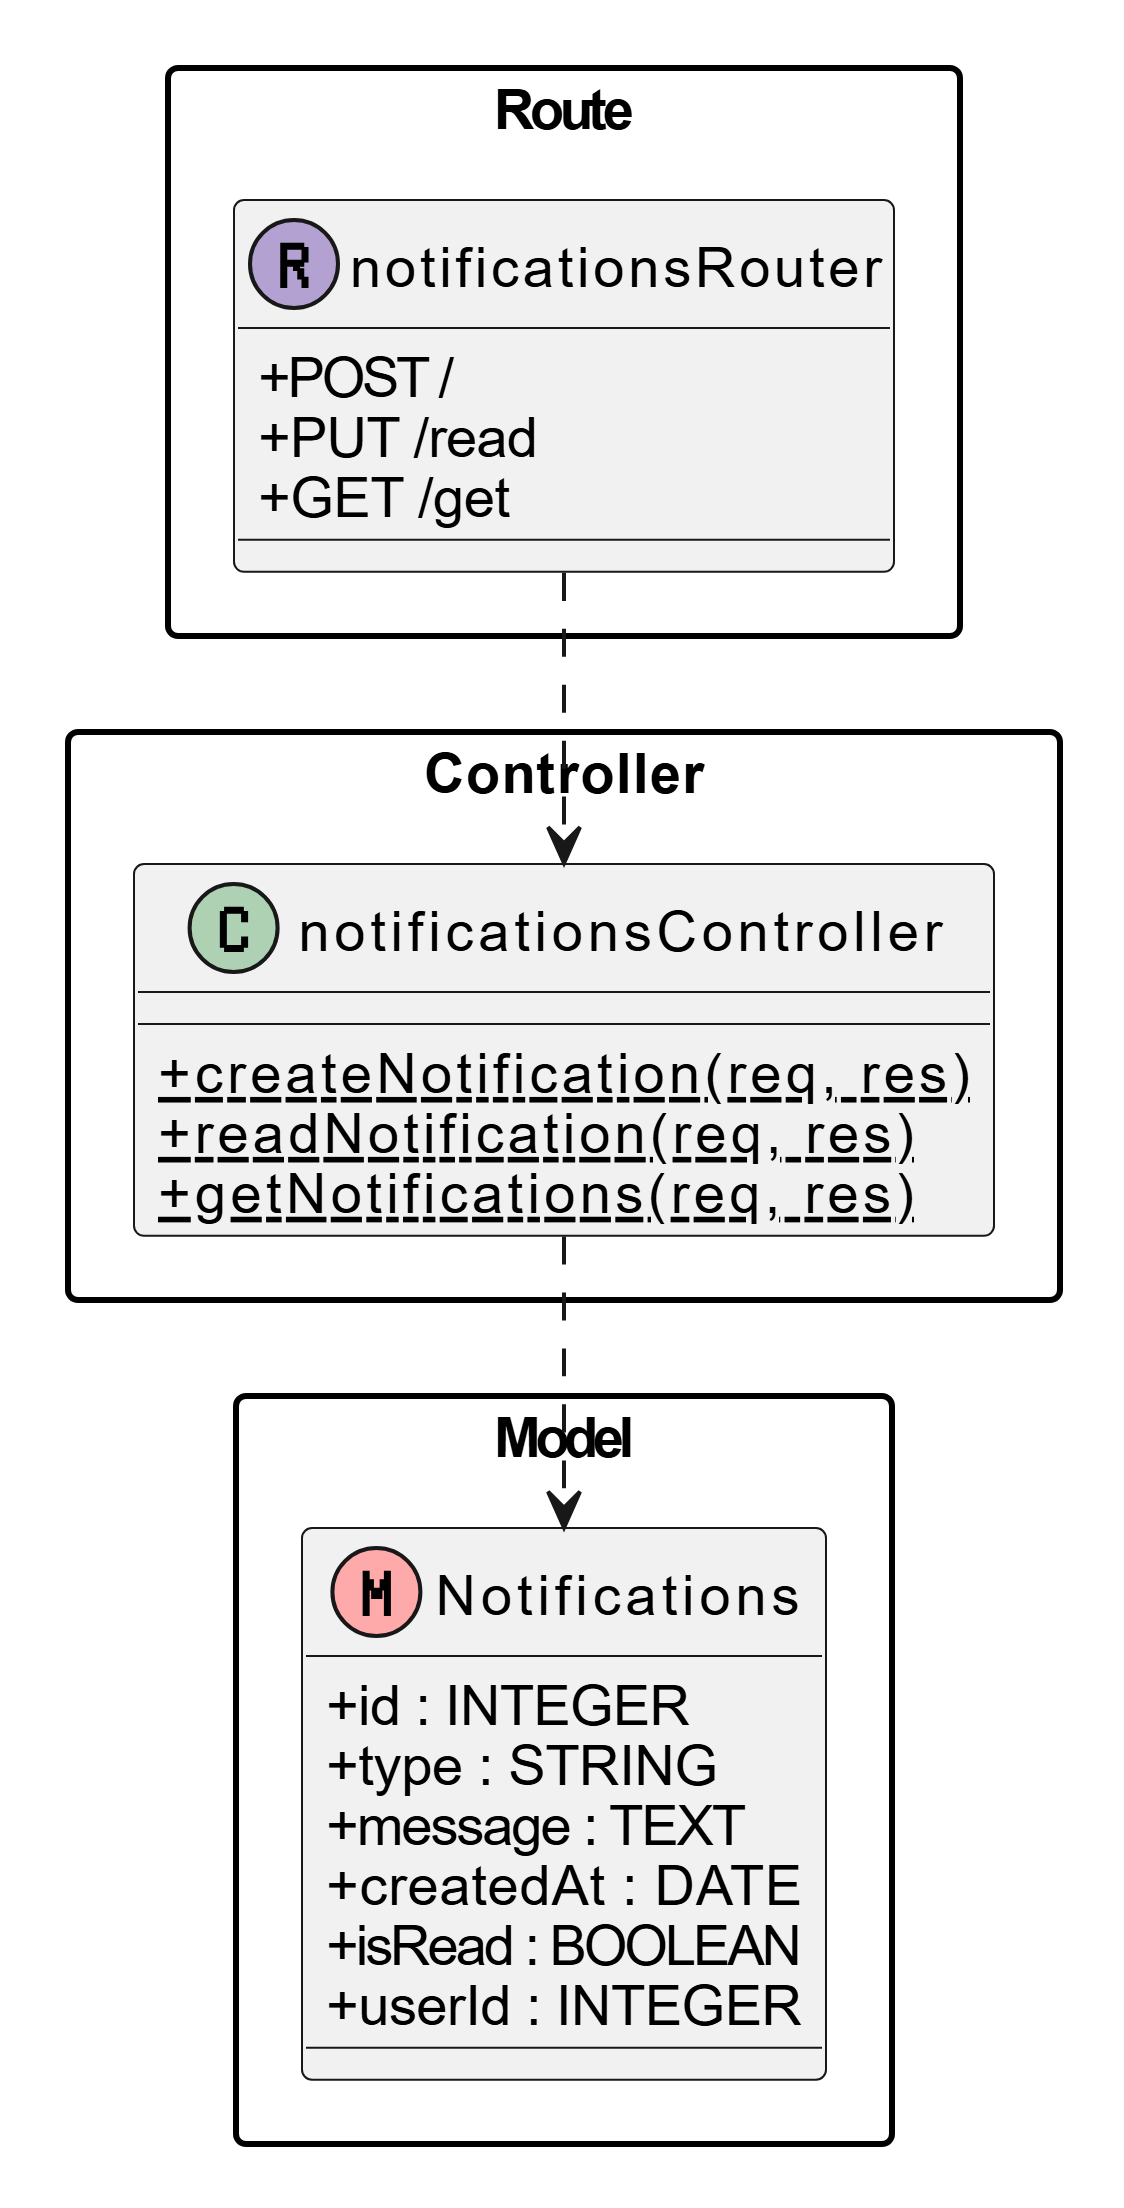
\includegraphics[width=0.5\textwidth]{images/fotoUML/NotificationsUML.png}
    \caption{Schema UML Notifications}
\end{figure}
\newpage

\subsubsection{Diagramma UML del modello "Searches"}
\begin{figure}[H]
    \centering
    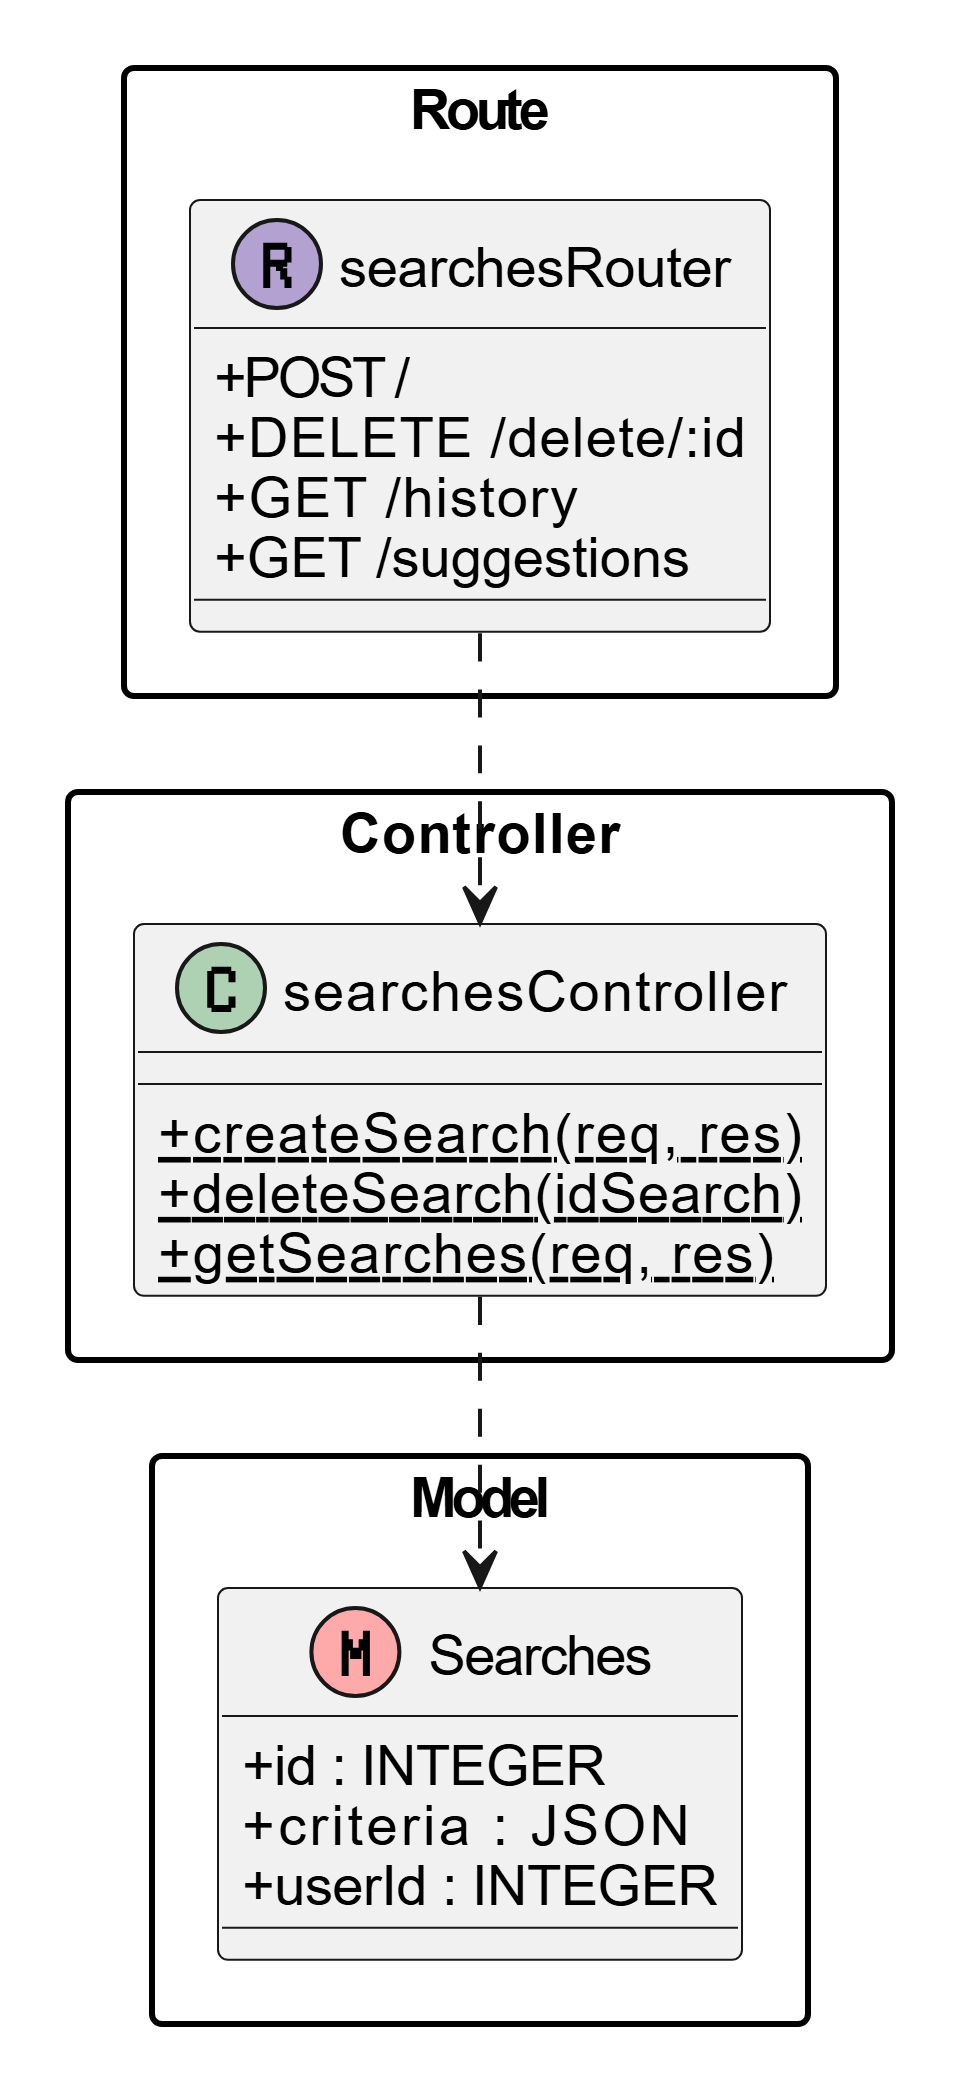
\includegraphics[width=0.5\textwidth]{images/fotoUML/SearchesUML.png}
    \caption{Schema UML Searches}
\end{figure}
\newpage

\subsection{Diagrammi di sequenza di design}

In questa sezione vengono presentati i \textbf{Diagrammi di Sequenza} per illustrare la dinamica del sistema catturando le interazioni temporali tra gli oggetti per i casi d'uso principali. Mentre il diagramma delle classi offre una visione statica dell'architettura, questi schemi documentano il \textbf{flusso logico dei messaggi}: dalla richiesta iniziale inviata dall'utente attraverso gli endpoint delle API, passando per le logiche di validazione e autorizzazione gestite dai middleware, fino alla persistenza dei dati tramite l'ORM (Sequelize) e la conseguente risposta al client.
\vspace{0.25cm} % Spaziatura verticale
\noindent % Disabilita l'indentazione del nuovo paragrafo
Sono stati analizzati e modellati i flussi critici per le diverse tipologie di attori (Admin, Agente, Utente), con particolare riferimento a:
\begin{itemize}
    \item \textbf{Gestione Immobili:} Processi di caricamento e aggiornamento delle proprietà e delle relative caratteristiche tecniche.
    \item \textbf{Creazione account agente immobiliare:} Flusso di creazione di un nuovo account Agente da parte di un Amministratore di Agenzia.
    \item \textbf{Ricerca Avanzata:} Ricerca sul catalogo immobiliare tramite filtri avanzati o l'uso di una mappa.
\end{itemize}

\vspace{0.25cm} % Spaziatura verticale
\noindent % Disabilita l'indentazione del nuovo paragrafo
\begin{tcolorbox}[colback=gray!10,colframe=black,title=Nota schema UML]
    Il processo di "Ricerca Immobile" è stato suddiviso in diagrammi distinti (Ricerca per Mappa, Ricerca per Filtri e Ricerca per Prezzo). Questa scelta è stata adottata per ridurre la complessità visiva dei singoli schemi, facilitando la comprensione granulare di come i diversi parametri di input interagiscano con il controller e il database per restituire i risultati filtrati.
\end{tcolorbox}

\subsection{Diagramma di sequenza aggiornamento immobile}
\begin{figure}[H]
    \centering
    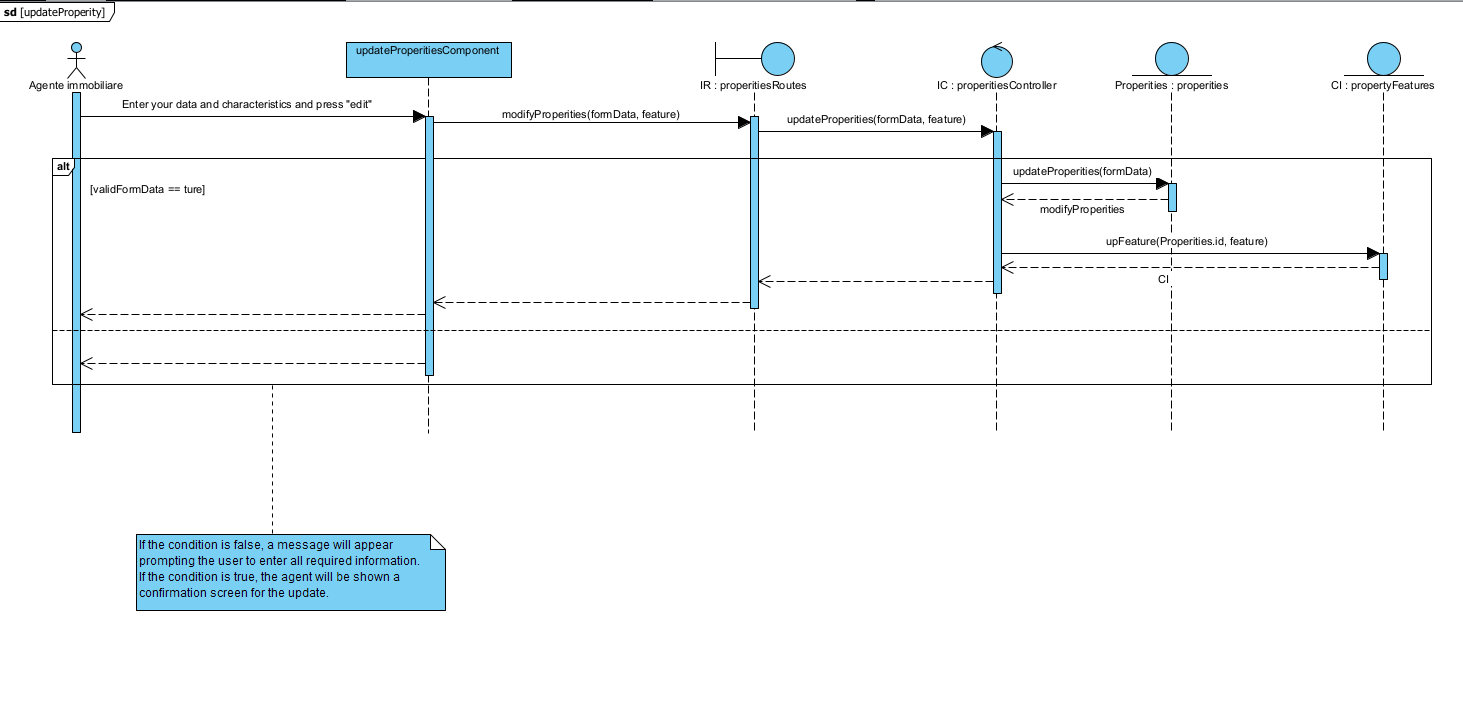
\includegraphics[width=1.1\textwidth]{images/fotoSequenceDiagram/aggiornametoImmobile.png}
    \caption{Schema UML Searches}
\end{figure}

\newpage
\subsection{Diagramma di sequenza caricamento immobile}
\begin{figure}[H]
    \centering
    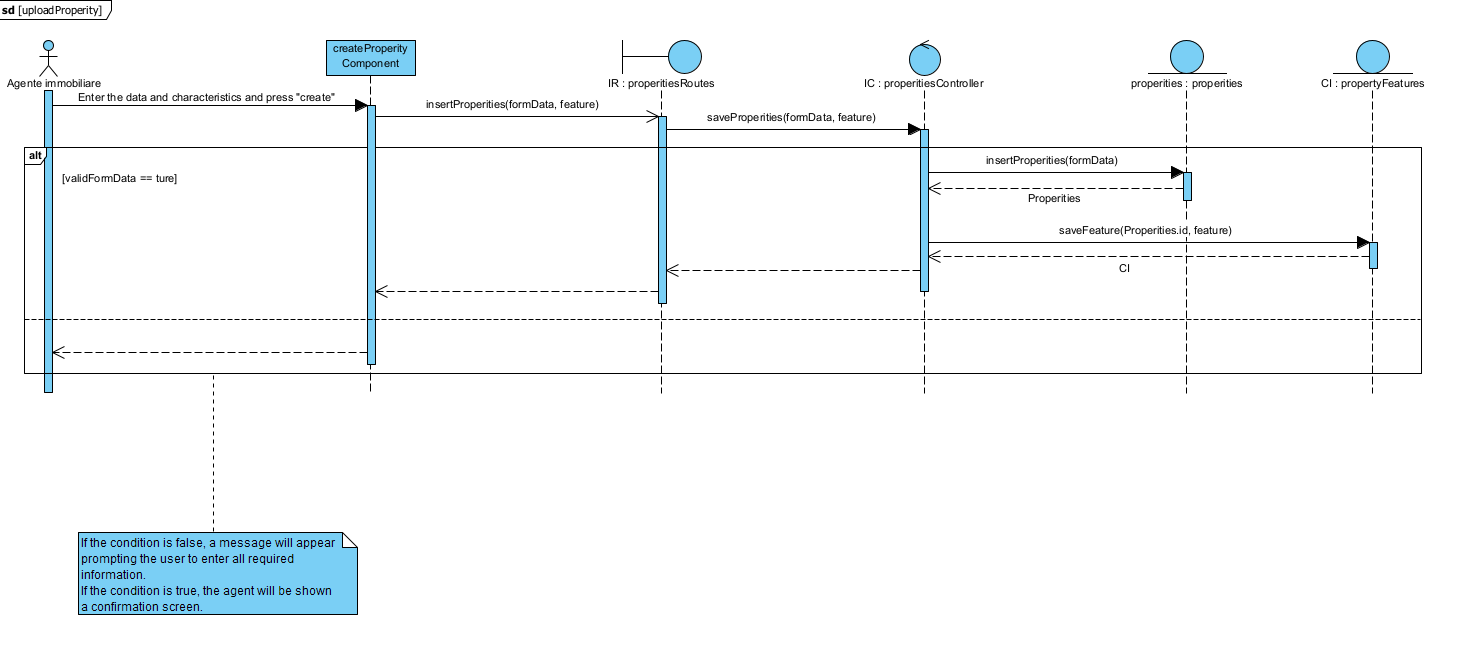
\includegraphics[width=1.1\textwidth]{images/fotoSequenceDiagram/caricamentoImmobile.png}
    \caption{Schema UML Searches}
\end{figure}
\newpage

\subsection{Diagramma di sequenza creazione agente immobiliare}
\begin{figure}[H]
    \centering
    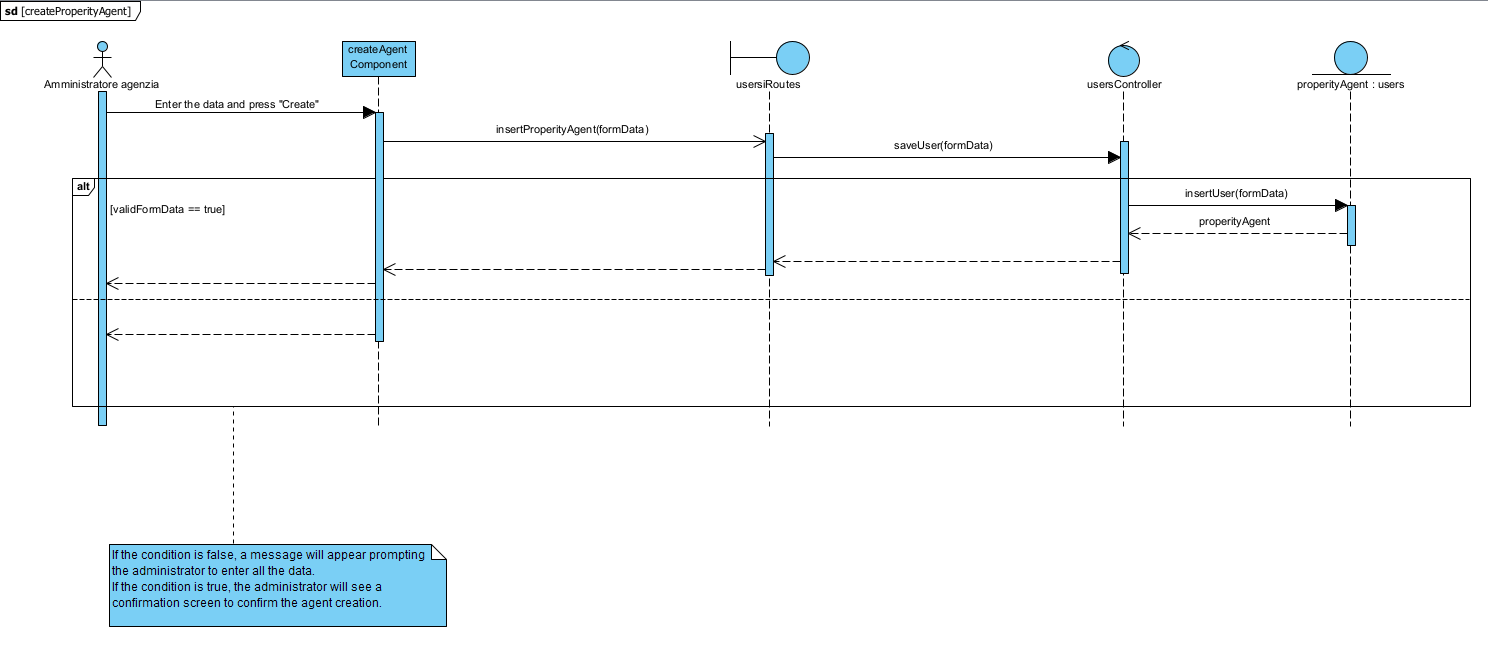
\includegraphics[width=1.1\textwidth]{images/fotoSequenceDiagram/creazioneAgenteImmobiliare.png}
    \caption{Schema UML Searches}
\end{figure}
\newpage

\subsection{Diagramma di sequenza ricerca immobile}
\begin{figure}[H]
    \centering
    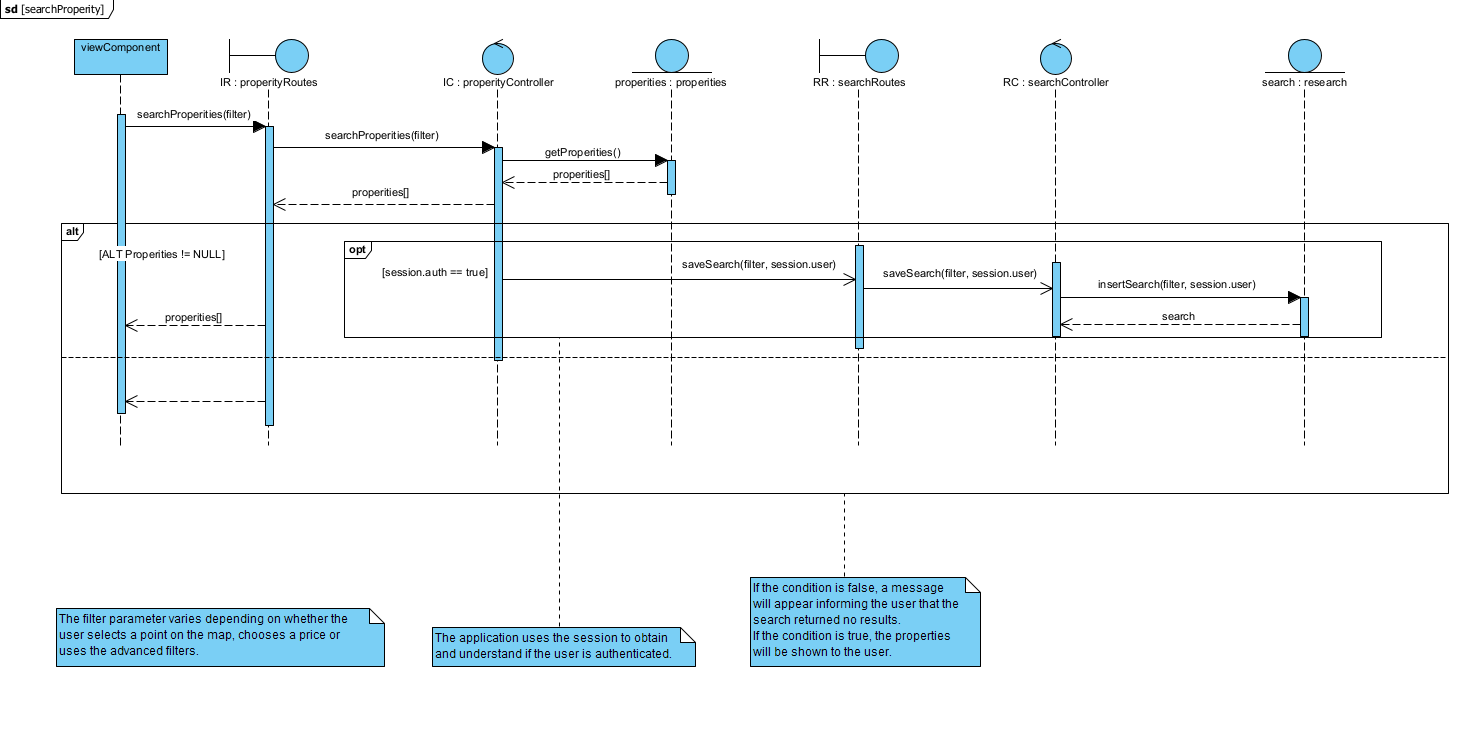
\includegraphics[width=1.1\textwidth]{images/fotoSequenceDiagram/ricercaImmobile.png}
    \caption{Schema UML Searches}
\end{figure}

\newpage

\subsection{Diagramma di sequenza ricerca tramite prezzo}
\begin{figure}[H]
    \centering
    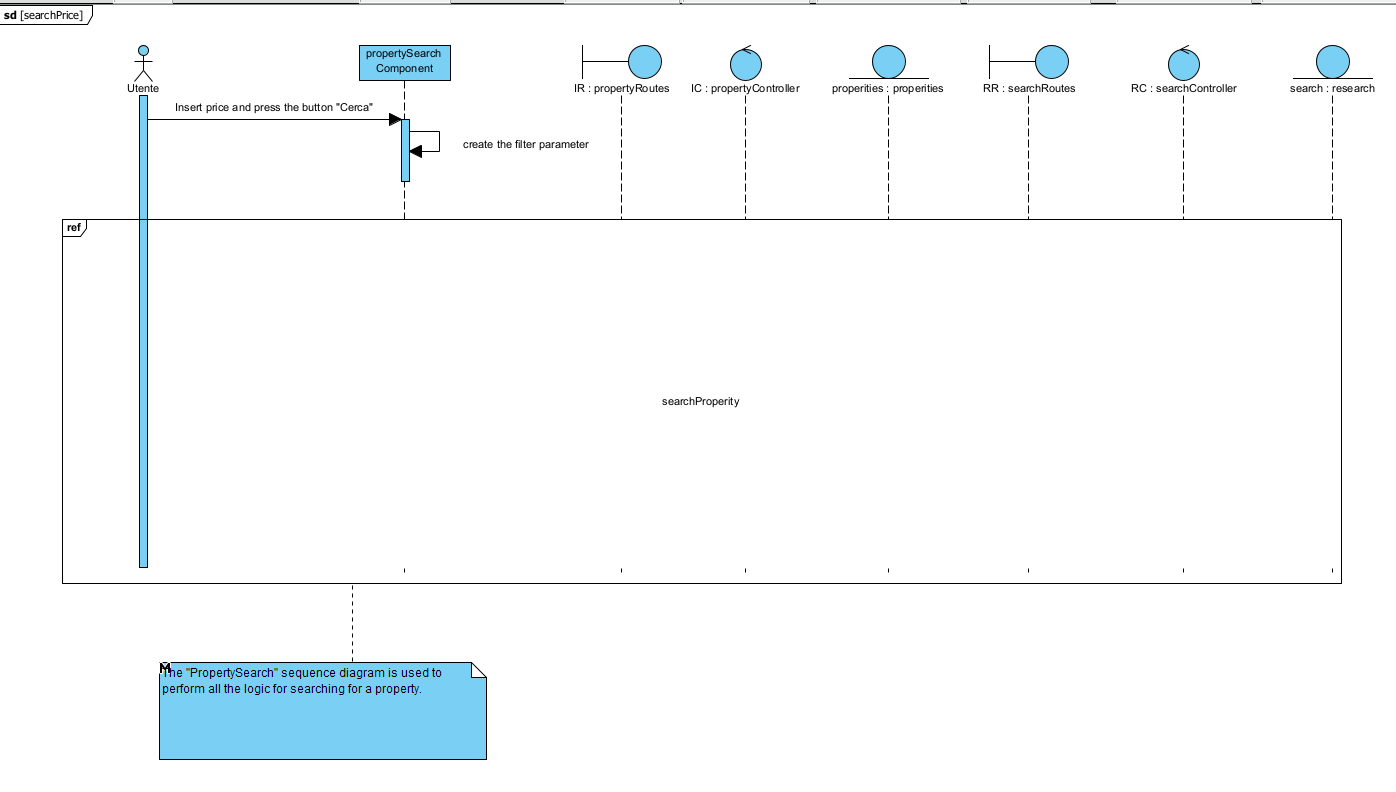
\includegraphics[width=1.1\textwidth]{images/fotoSequenceDiagram/ricercaPrezzo.png}
    \caption{Schema UML Searches}
\end{figure}

\newpage

\subsection{Diagramma di sequenza ricerca tramite mappa}
\begin{figure}[H]
    \centering
    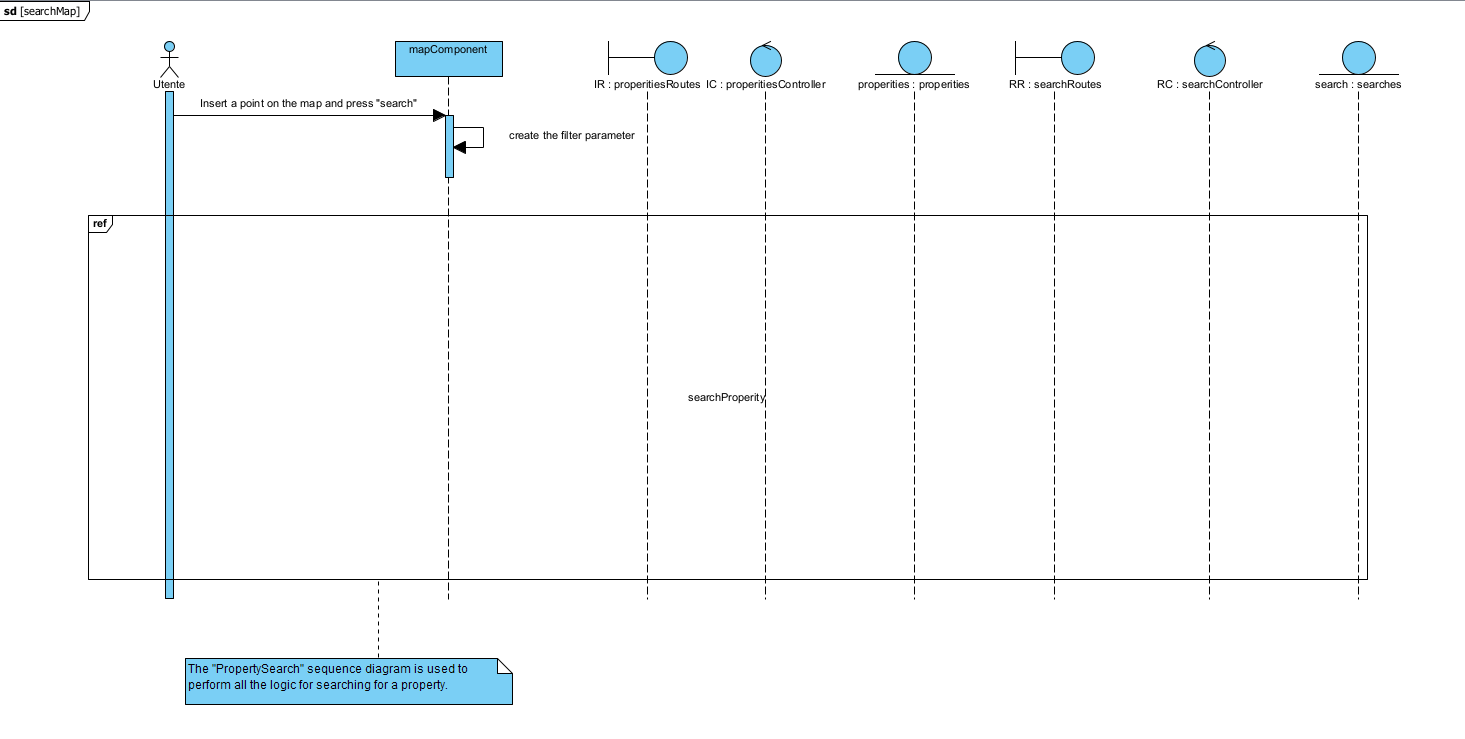
\includegraphics[width=1.1\textwidth]{images/fotoSequenceDiagram/ricercaMappa.png}
    \caption{Schema UML Searches}
\end{figure}

\newpage

\subsection{Diagramma di sequenza ricerca tramite filtri}
\begin{figure}[H]
    \centering
    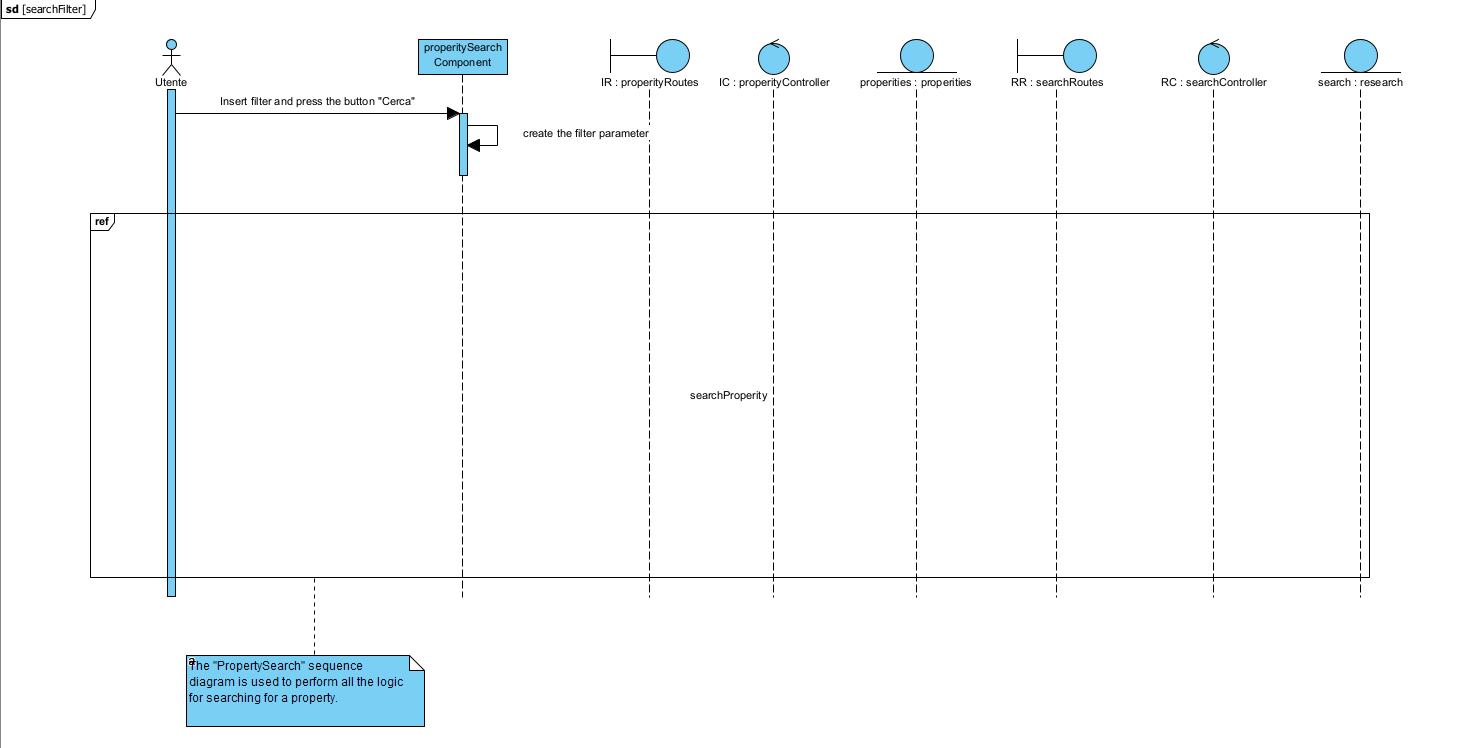
\includegraphics[width=1.1\textwidth]{images/fotoSequenceDiagram/ricercaFiltri.png}
    \caption{Schema UML Searches}
\end{figure}

\newpage

\subsection{Sistema di versionamento}
Per il versionamento del codice abbiamo utilizzato come tecnologia github, che ci ha permesso di gestire in modo efficiente le modifiche al codice sorgente, facilitando la collaborazione tra i membri del team e mantenendo una cronologia dettagliata delle evoluzioni del progetto. Tutto il progetto è stato messo su una unica repository suddivisa in backend e frontend. Di seguito viene riportato un estratto di tutti i commit effettuati durante lo sviluppo.
\begin{figure}[H]
    \centering
    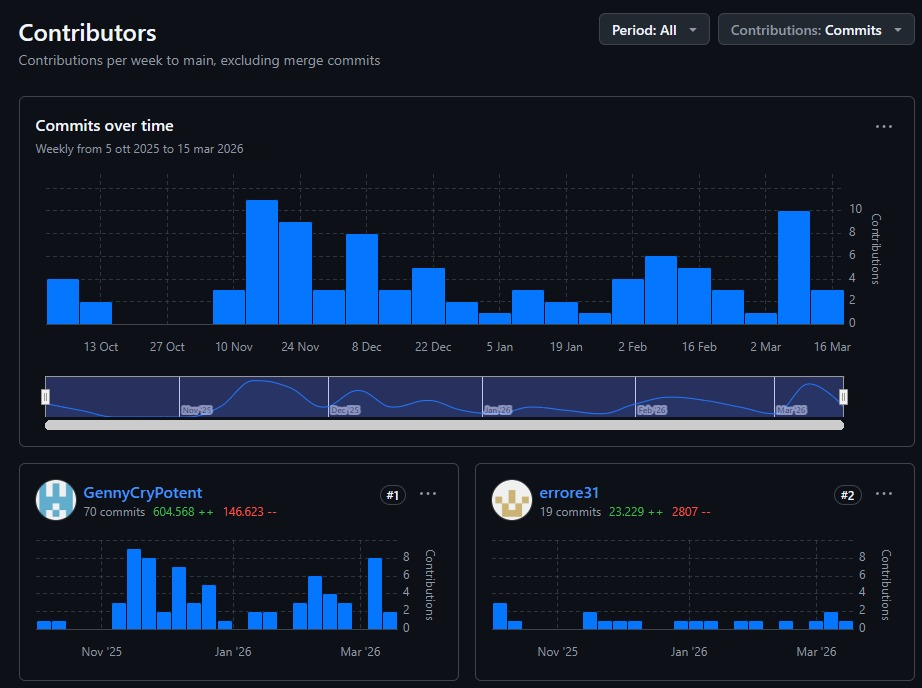
\includegraphics[width=1\textwidth]{images/CommitGitHub.jpeg}
    \caption{Storia dei commit su GitHub}
\end{figure}


\newpage
\subsubsection{Report della qualità del codice}
Per garantire la qualità del codice, è stato utilizzato SonarQube, un tool di analisi statica del codice che ci ha permesso di identificare e risolvere potenziali problemi di qualità e di mantenere un alto livello di standardizzazione del codice. Di seguito è riportato un estratto del report generato da SonarQube, evidenziando le metriche chiave relative alla copertura dei test, alla complessità del codice e alla presenza di eventuali bug o code smells.
\begin{figure}[H]
    \centering
    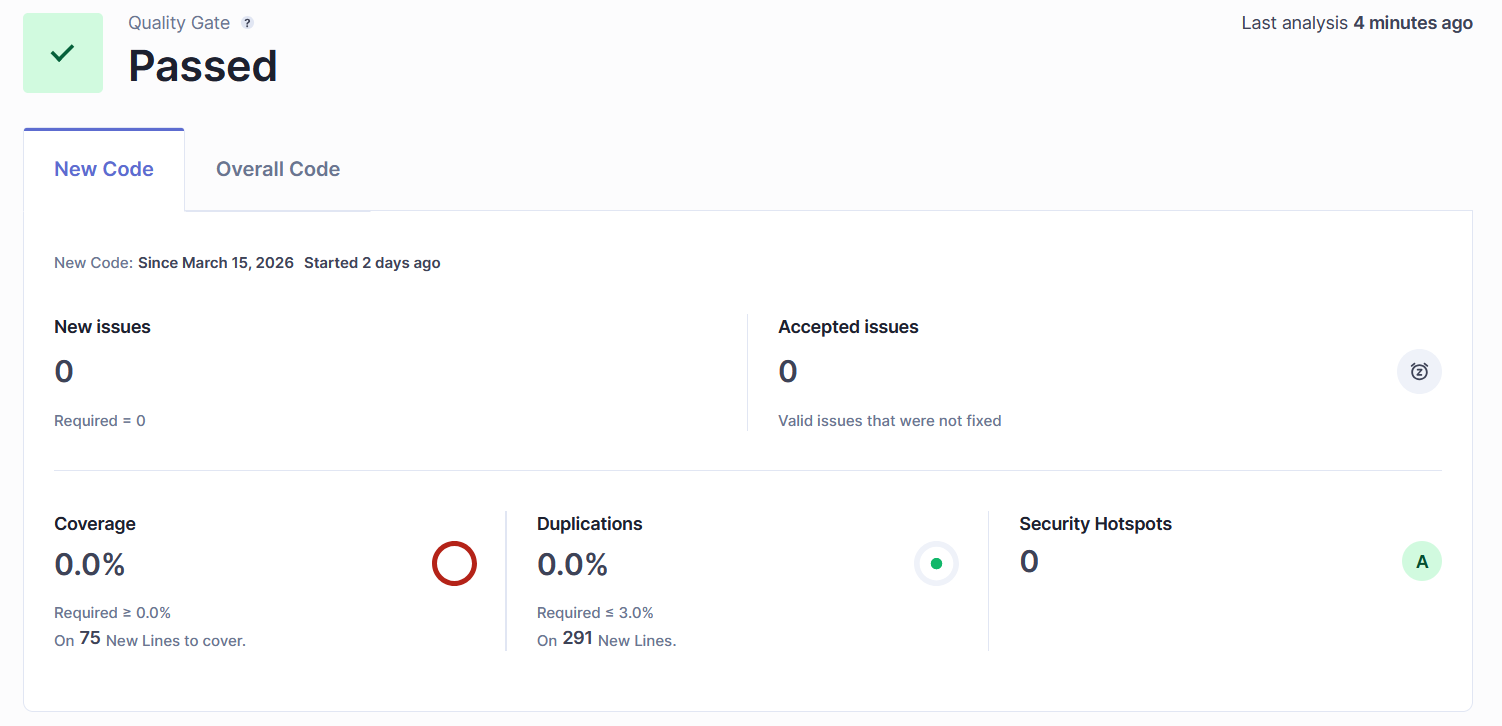
\includegraphics[width=1\textwidth]{images/ReportSonarQube.png}
    \caption{Report di qualità del codice su SonarQube}
\end{figure}


\newpage

\section{Testing}
La fase di testing ha l'obiettivo di garantire che i moduli software sviluppati rispondano correttamente ai requisiti funzionali individuati in fase di analisi. La di verifica si è concentrata sulla ricerca di eventuali difetti logici e sulla validazione della robustezza del backend, assicurando che il sistema sia in grado di gestire correttamente non solo gli input validi, ma anche situazioni di errore o casi limite.

\subsection{Strategia e tecnologie}
Per la fase di verifica del backend, sviluppato in Node.js, è stato adottato il framework \textbf{Jasmine}, che ha permesso l'implementazione di unit test conformi allo standard xUnit. La strategia di testing è stata focalizzata su un approccio puramente funzionale, integrando metodiche avanzate per garantire la massima affidabilità delle componenti critiche.

Di seguito sono descritti i pilastri metodologici utilizzati:

\begin{itemize}
    \item \textbf{Approccio Signature-based}: I test sono stati progettati basandosi esclusivamente sulla \textit{firma} dei metodi (parametri di input e tipi di ritorno). Questo ha permesso di validare l'interfaccia dei controller garantendo che il sistema risponda correttamente alle sollecitazioni esterne previste dal contratto software.

    \item \textbf{Copertura R-WECT} (\textit{Robust Weak Equivalence Class Testing}): Si è scelto questo specifico approccio di partizione per bilanciare efficacia e manutenibilità.
          \begin{itemize}
              \item \textbf{Weak (Debole)}: Si assume che le anomalie siano causate raramente dalla combinazione simultanea di più errori; pertanto, ogni test case sollecita una sola classe invalida alla volta, mantenendo gli altri parametri entro i range di validità.
              \item \textbf{Robust (Robusta)}: A differenza del WECT standard, questa variante include esplicitamente il testing delle \textbf{classi di errore} (input nulli, fuori range o malformati), garantendo che il backend gestisca le eccezioni senza crash di sistema.
          \end{itemize}

    \item \textbf{Analisi dei Valori al Limite} (\textit{Boundary Value Analysis}): Integrata alla partizione in classi, questa tecnica è stata fondamentale per verificare il comportamento del sistema in corrispondenza delle soglie critiche (es. lunghezze minime delle password o soglie di prezzo per il contratto), dove statisticamente si annida la maggior parte dei bug logici.
\end{itemize}

\newpage

\subsection{Metodi di test}
In questa sezione vengono illustrati i casi di test relativi a quattro componenti core del sistema, selezionati per l'articolazione della loro logica di business e per la criticità rivestita nel mantenimento dell'integrità dei dati.

\subsubsection{TEST 1: Registrazione utente}
\begin{lstlisting}[language=javascript, caption=Unit Test della logica di registrazione]
 validateRegistration: (email, password, role) => {
        const emailRegex = /^[^\s@]+@[^\s@]+\.[^\s@]+$/;
        const validRoles = ['User', 'Agency', 'Admin'];

        if (!emailRegex.test(email)) return "EMAIL_INVALIDA";
        if (!password || password.length < 8) return "PASSWORD_TROPPO_CORTA";
        if (!validRoles.includes(role)) return "RUOLO_NON_VALIDO";
        
        return "REGISTRAZIONE_OK";
    }

describe("Metodo: validateRegistration", () => {
        it("TC_01 - Email errata", () => {
            const result = TestTarget.validateRegistration("mario.rossi", "Segreta123", "User");
            expect(result).toBe("EMAIL_INVALIDA");
        });
        it("TC_02 - Password troppo corta", () => {
            const result = TestTarget.validateRegistration("mario@email.it", "Pass123", "User");
            expect(result).toBe("PASSWORD_TROPPO_CORTA");
        });
        it("TC_03 - Ruolo non valido", () => {
            const result = TestTarget.validateRegistration("mario@email.it", "PasswordSicura123", "Guest");
            expect(result).toBe("RUOLO_NON_VALIDO");
        });
         it("TC_04 - Registrazione corretta", () => {
            const result = TestTarget.validateRegistration("mario@email.it", "PasswordSicura123", "User");
            expect(result).toBe("REGISTRAZIONE_OK");
        });
    });
\end{lstlisting}

\begin{itemize}
    \item \textbf{email}: Stringa rappresentante l'indirizzo di posta elettronica dell'utente. Viene validata tramite espressione regolare per garantirne il formato standard.
    \item \textbf{password}: Stringa alfanumerica scelta dall'utente. Il sistema impone un vincolo di sicurezza minimo di 8 caratteri.
    \item \textbf{role}: Stringa che definisce il livello di accesso dell'account. I valori ammessi sono limitati a un set predefinito: \texttt{'User'}, \texttt{'Agency'}, \texttt{'Admin'}.
\end{itemize}

\paragraph{Strategia Adottata} \mbox{} \\
Strategia \textbf{Black Box} con approccio \textbf{signature-based} e copertura \textbf{R-WECT}. La logica di test è focalizzata sulla validazione dei vincoli d'integrità del profilo utente: si verifica il corretto filtraggio delle email tramite espressioni regolari e la gestione della sicurezza della password, assicurando che il sistema rifiuti ruoli non previsti dal dominio applicativo.

\newpage

\renewcommand{\arraystretch}{1.5}
\begin{table}[H]
    \centering
    \caption{Classi di Equivalenza - validateRegistration}
    \begin{tabularx}{\textwidth}{|l|X|c|c|}
        \hline
        \rowcolor{DarkBlue}
        \textbf{\color{white}Parametro} & \textbf{\color{white}Classe di Equivalenza}         & \textbf{\color{white}Validità} & \textbf{\color{white}ID CE} \\ \hline
        \rowcolor[gray]{0.95}
        \textit{email}                  & Formato sintatticamente corretto (es. user@test.it) & Valida                         & CE1                         \\ \hline
        \textit{email}                  & Formato mancante di @ o dominio (es. user.it)       & Invalida                       & CE2                         \\ \hline
        \rowcolor[gray]{0.95}
        \textit{password}               & Lunghezza superiore o uguale a 8 caratteri          & Valida                         & CE3                         \\ \hline
        \textit{password}               & Lunghezza inferiore a 8 caratteri                   & Invalida                       & CE4                         \\ \hline
        \rowcolor[gray]{0.95}
        \textit{role}                   & Valore incluso nel set \{User, Agency, Admin\}      & Valida                         & CE5                         \\ \hline
        \textit{role}                   & Valore non censito o nullo                          & Invalida                       & CE6                         \\ \hline
    \end{tabularx}
\end{table}

\begin{table}[H]
    \centering
    \caption{Matrice dei Casi di Test - validateRegistration}
    \rowcolors{2}{white}{gray!10}
    \begin{tabularx}{\textwidth}{|l|l|X|l|l|}
        \hline
        \rowcolor{DarkBlue}
        \textbf{\color{white}ID Test} & \textbf{\color{white}CE Rif.} & \textbf{\color{white}Input (email, psw, role)}   & \textbf{\color{white}Output Atteso} & \textbf{\color{white}Esito}      \\ \hline
        \textbf{TC\_01}               & CE2 + CE3 + CE5               & ("mario.rossi", "Segreta123", "User")            & EMAIL\_INVALIDA                     & {\color{codegreen}\textbf{PASS}} \\ \hline
        \textbf{TC\_02}               & CE1 + CE4 + CE5               & ("mario@email.it", "Pass123", "User")            & PASSWORD\_TROPPO\_CORTA             & {\color{codegreen}\textbf{PASS}} \\ \hline
        \textbf{TC\_03}               & CE1 + CE3 + CE6               & ("mario@email.it", "PasswordSicura123", "Guest") & RUOLO\_NON\_VALIDO                  & {\color{codegreen}\textbf{PASS}} \\ \hline
        \textbf{TC\_04}               & CE1 + CE3 + CE5               & ("mario@email.it", "PasswordSicura123", "User")  & REGISTRAZIONE\_OK                   & {\color{codegreen}\textbf{PASS}} \\ \hline
    \end{tabularx}
\end{table}

\newpage
\subsubsection{TEST 2: Controllo input creazione proprietà}
\begin{lstlisting}[language=javascript, caption=Unit Test della logica di validione input proprietà]
 checkPropertyConstraints: (price, contractType, description) => {
        if (!price || price <= 0) return "PREZZO_NON_VALIDO";
        if (!description || description.length < 10) return "DESCRIZIONE_INSUFFICIENTE";
        
        // Logica di business: coerenza prezzo/contratto
        if (contractType === 'Affitto' && price > 5000) return "ANOMALIA_PREZZO_AFFITTO";
        if (contractType === 'Vendita' && price < 10000) return "ANOMALIA_PREZZO_VENDITA";
        
        return "VALIDO";
    },

describe("Metodo: checkPropertyConstraints", () => {
        it("TC_05 - Descrizione troppo breve", () => {
            const result = TestTarget.checkPropertyConstraints(150000, 'Vendita', 'Casa');
            expect(result).toBe("DESCRIZIONE_INSUFFICIENTE");
        });
        it("TC_06 - Prezzo incoerente per affitto", () => {
            const result = TestTarget.checkPropertyConstraints(6000, 'Affitto', 'Bellissimo attico panoramico');
            expect(result).toBe("ANOMALIA_PREZZO_AFFITTO");
        });
        it("TC_07 - Inserimento giusto", () => {
            const result = TestTarget.checkPropertyConstraints(3000, 'Affitto', 'Bellissimo attico panoramico');
            expect(result).toBe("VALIDO");
        });
    });
\end{lstlisting}

\begin{itemize}
    \item \textbf{price}: Valore numerico indicante il costo dell'immobile. Deve essere un numero positivo e coerente con la tipologia di contratto scelta.
    \item \textbf{contractType}: Stringa che definisce la natura della transazione. I valori ammessi (in linea con i validatori del backend) sono \texttt{'Affitto'} e \texttt{'Vendita'}.
    \item \textbf{description}: Stringa descrittiva dell'immobile. Per garantire la qualità degli annunci, il sistema impone una lunghezza minima di 10 caratteri.
\end{itemize}

\paragraph{Strategia Adottata} \mbox{} \\
Strategia \textbf{Black Box} con approccio \textbf{signature-based} e copertura \textbf{R-WECT}. In questo scenario, il testing mira a garantire la solidità delle \textbf{regole di business}. Si verifica che il sistema intercetti le anomalie tra prezzo e tipologia di contratto (evitando, ad esempio, prezzi di vendita irrisori o affitti fuori mercato) e che non vengano accettate descrizioni troppo brevi per gli annunci.

\newpage

\renewcommand{\arraystretch}{1.5}
\begin{table}[H]
    \centering
    \caption{Classi di Equivalenza - checkPropertyConstraints}
    \begin{tabularx}{\textwidth}{|l|X|c|c|}
        \hline
        \rowcolor{DarkBlue}
        \textbf{\color{white}Parametro} & \textbf{\color{white}Classe di Equivalenza}      & \textbf{\color{white}Validità} & \textbf{\color{white}ID CE} \\ \hline
        \rowcolor[gray]{0.95}
        \textit{price}                  & Valore numerico strettamente positivo ($> 0$)    & Valida                         & CE7                         \\ \hline
        \textit{price}                  & Valore nullo, negativo o non numerico            & Invalida                       & CE8                         \\ \hline
        \rowcolor[gray]{0.95}
        \textit{description}            & Lunghezza della stringa $\geq 10$ caratteri      & Valida                         & CE9                         \\ \hline
        \textit{description}            & Lunghezza della stringa $< 10$ caratteri         & Invalida                       & CE10                        \\ \hline
        \rowcolor[gray]{0.95}
        \textit{contractType}           & Prezzo $> 5000$ con contratto di tipo 'Affitto'  & Invalida                       & CE11                        \\ \hline
        \textit{contractType}           & Prezzo $< 10000$ con contratto di tipo 'Vendita' & Invalida                       & CE12                        \\ \hline
    \end{tabularx}
\end{table}

\begin{table}[H]
    \centering
    \caption{Matrice dei Casi di Test - checkPropertyConstraints}
    \rowcolors{2}{white}{gray!10}
    \begin{tabularx}{\textwidth}{|l|c|X|l|l|}
        \hline
        \rowcolor{DarkBlue}
        \textbf{\color{white}ID Test} & \textbf{\color{white}CE Rif.} & \textbf{\color{white}Input (price, type, desc)}   & \textbf{\color{white}Output Atteso} & \textbf{\color{white}Esito}      \\ \hline
        \textbf{TC\_05}               & CE7 + CE10                    & (150000, 'Vendita', 'Casa')                       & DESCRIZIONE\_INSUFFICIENTE          & {\color{codegreen}\textbf{PASS}} \\ \hline
        \textbf{TC\_06}               & CE7 + CE11 + CE9              & (6000, 'Affitto', 'Bellissimo attico panoramico') & ANOMALIA\_PREZZO\_AFFITTO           & {\color{codegreen}\textbf{PASS}} \\ \hline
        \textbf{TC\_07}               & CE7 + CE9                     & (3000, 'Affitto', 'Bellissimo attico panoramico') & VALIDO                              & {\color{codegreen}\textbf{PASS}} \\ \hline
    \end{tabularx}
\end{table}

\newpage
\subsubsection{TEST 3: Matching Località}
\begin{lstlisting}[language=javascript, caption=Unit Test della logica di matching della ricerca con la località ]
checkMatch: (propertyAddress, searchString) => {
    if (!propertyAddress || !searchString) return false;
    const searchTerm = searchString.split(',')[0].trim().toLowerCase();
    return propertyAddress.toLowerCase().includes(searchTerm);
},

describe("Metodo: checkMatch", () => {
   it("TC_08 - Dovrebbe matchare la localita ignorando spazi e case", () => {
        expect(TestTarget.checkMatch("Via Roma 10, Napoli", "NAPOLI , NA")).toBeTrue();
    });
    it("TC_09 - Dovrebbe restituire false se la localita non matcha", () => {
        expect(TestTarget.checkMatch("Via Roma 10, Napoli", "Milano, MI")).toBeFalse();
    });
    it("TC_10 - Dovrebbe restituire false con i parametri nulli", () => {
        expect(TestTarget.checkMatch(null, "Napoli, NA")).toBeFalse();
        expect(TestTarget.checkMatch("Via Roma 10, Napoli", null)).toBeFalse();
    });
});
\end{lstlisting}

\begin{itemize}
    \item \textbf{propertyAddress}: Stringa contenente l'indirizzo completo dell'immobile (es. "Via Roma 10, Napoli").
    \item \textbf{searchString}: Stringa di ricerca inserita dall'utente, che può contenere informazioni aggiuntive separate da virgole (es. "Napoli, NA, Italia").
\end{itemize}

\paragraph{Strategia Adottata} \mbox{} \\
Strategia \textbf{Black Box} con approccio \textbf{signature-based} e copertura \textbf{R-WECT}. La strategia è volta a testare l'algoritmo di manipolazione delle stringhe di ricerca. Viene verificata la capacità della funzione di normalizzare l'input dell'utente, garantendo un matching efficace indipendentemente dalla capitalizzazione (\textit{case-insensitivity}), dalla presenza di spazi superflui o dall'inserimento di dettagli geografici aggiuntivi dopo la virgola.

\newpage
\renewcommand{\arraystretch}{1.5}
\begin{table}[H]
    \centering
    \caption{Classi di Equivalenza - checkMatch}
    \begin{tabularx}{\textwidth}{|l|X|c|c|}
        \hline
        \rowcolor{DarkBlue}
        \textbf{\color{white}Parametro} & \textbf{\color{white}Classe di Equivalenza}           & \textbf{\color{white}Validità} & \textbf{\color{white}ID CE} \\ \hline
        \rowcolor[gray]{0.95}
        \textit{propertyAddress}        & Stringa indirizzo valida (es. "Via Roma")             & Valida                         & CE13                        \\ \hline
        \textit{propertyAddress}        & Valore nullo o non definito (\texttt{null})           & Invalida                       & CE14                        \\ \hline
        \rowcolor[gray]{0.95}
        \textit{searchString}           & Sottostringa presente nell'indirizzo                  & Valida                         & CE15                        \\ \hline
        \textit{searchString}           & Sottostringa NON presente nell'indirizzo              & Valida                         & CE16                        \\ \hline
        \rowcolor[gray]{0.95}
        \textit{searchString}           & Formato con spazi/maiuscole/virgole (es. " NAPOLI ,") & Valida                         & CE17                        \\ \hline
        \textit{searchString}           & Valore nullo o non definito (\texttt{null})           & Invalida                       & CE18                        \\ \hline
    \end{tabularx}
\end{table}

\begin{table}[H]
    \centering
    \caption{Matrice dei Casi di Test - checkMatch}
    \rowcolors{2}{white}{gray!10}
    \begin{tabularx}{\textwidth}{|l|c|X|X|c|}
        \hline
        \rowcolor{DarkBlue}
        \textbf{\color{white}ID Test} & \textbf{\color{white}CE Rif.} & \textbf{\color{white}Input (address, search)} & \textbf{\color{white}Output Atteso} & \textbf{\color{white}Esito}      \\ \hline
        \textbf{TC\_08}               & CE13 + CE15 + CE17            & ("Via Roma 10, Napoli", "NAPOLI , NA")        & \texttt{true}                       & {\color{codegreen}\textbf{PASS}} \\ \hline
        \textbf{TC\_09}               & CE13 + CE16 + CE17            & ("Via Roma 10, Napoli", "Milano, MI")         & \texttt{false}                      & {\color{codegreen}\textbf{PASS}} \\ \hline
        \textbf{TC\_10}               & CE14 + CE18                   & (\texttt{null}, \texttt{null})                & \texttt{false}                      & {\color{codegreen}\textbf{PASS}} \\ \hline
    \end{tabularx}
\end{table}
\newpage
\subsubsection{TEST 4: Generazione titolo notifica}
\begin{lstlisting}[language=javascript, caption=Unit Test della logica di Generazione del titolo della notifica]
generateNotificationText: (type, propertyTitle) => {
    if (!propertyTitle) return "Nuova Notifica";
    const title = propertyTitle.toUpperCase();
    
    if (type === 'promo') return `OFFERTA SPECIALE: ${title}`;
    if (type === 'property') return `CORRISPONDENZA TROVATA: ${title}`;
    return `Aggiornamento su ${title}`;
}

describe("Metodo: generateNotificationText", () => {
    it("TC_11 - Dovrebbe formattare il titolo in maiuscolo per le promo", () => {
        const result = TestTarget.generateNotificationText('promo', 'Appartamento centro');
        expect(result).toBe("OFFERTA SPECIALE: APPARTAMENTO CENTRO");
    });
    it("TC_12 - Dovrebbe formattare il titolo in maiuscolo per le property", () => {
        const result = TestTarget.generateNotificationText('property', 'Villa con piscina');
        expect(result).toBe("CORRISPONDENZA TROVATA: VILLA CON PISCINA");
    });
    it("TC_13 - Dovrebbe restituire un titolo generico se il titolo della proprieta e mancante", () => {
        const result = TestTarget.generateNotificationText('promo', '');
        expect(result).toBe("Nuova Notifica");
    });
});
\end{lstlisting}

\begin{itemize}
    \item \textbf{type}: Stringa che definisce la categoria della notifica[cite: 202]. Determina il prefisso del messaggio (es. \texttt{'promo'}, \texttt{'property'})[cite: 202].
    \item \textbf{propertyTitle}: Stringa contenente il nome dell'immobile[cite: 203]. Viene elaborata per essere visualizzata in maiuscolo all'interno del messaggio[cite: 203].
\end{itemize}

\paragraph{Strategia Adottata} \mbox{} \\
Strategia \textbf{Black Box} con approccio \textbf{signature-based} e copertura \textbf{R-WECT}. Il test si concentra sulla trasformazione dei dati per l'interfaccia utente (\textit{UI string processing}). Si convalida la corretta generazione dei prefissi dinamici in base al tipo di notifica e la trasformazione in maiuscolo del titolo, verificando inoltre la presenza di una logica di \textit{fallback} che garantisca un messaggio di default qualora i metadati dell'immobile fossero mancanti.

\newpage
\renewcommand{\arraystretch}{1.5}
\begin{table}[H]
    \centering
    \caption{Classi di Equivalenza - generateNotificationText}
    \begin{tabularx}{\textwidth}{|l|X|c|c|}
        \hline
        \rowcolor{DarkBlue}
        \textbf{\color{white}Parametro} & \textbf{\color{white}Classe di Equivalenza}       & \textbf{\color{white}Validità} & \textbf{\color{white}ID CE} \\ \hline
        \rowcolor[gray]{0.95}
        \textit{type}                   & Categoria promozionale (\texttt{'promo'})         & Valida                         & CE19                        \\ \hline
        \textit{type}                   & Categoria di corrispondenza (\texttt{'property'}) & Valida                         & CE20                        \\ \hline
        \rowcolor[gray]{0.95}
        \textit{type}                   & Qualsiasi altro valore (Categoria generica)       & Valida                         & CE21                        \\ \hline
        \textit{propertyTitle}          & Stringa titolo valida (non vuota)                 & Valida                         & CE22                        \\ \hline
        \rowcolor[gray]{0.95}
        \textit{propertyTitle}          & Stringa vuota o non definita (\texttt{null})      & Invalida                       & CE23                        \\ \hline
    \end{tabularx}
\end{table}

\begin{table}[H]
    \centering
    \caption{Matrice dei Casi di Test - generateNotificationText}
    \rowcolors{2}{white}{gray!10}
    \begin{tabularx}{\textwidth}{|l|c|X|X|c|}
        \hline
        \rowcolor{DarkBlue}
        \textbf{\color{white}ID Test} & \textbf{\color{white}CE Rif.} & \textbf{\color{white}Input (type, title)} & \textbf{\color{white}Output Atteso}         & \textbf{\color{white}Esito}      \\ \hline
        \textbf{TC\_11}               & CE19 + CE22                   & ('promo', 'Appartamento centro')          & 'OFFERTA SPECIALE: APPARTAMENTO CENTRO'     & {\color{codegreen}\textbf{PASS}} \\ \hline
        \textbf{TC\_12}               & CE20 + CE22                   & ('property', 'Villa con piscina')         & 'CORRISPONDENZA TROVATA: VILLA CON PISCINA' & {\color{codegreen}\textbf{PASS}} \\ \hline
        \textbf{TC\_13}               & CE19 + CE23                   & ('promo', '')                             & 'Nuova Notifica'                            & {\color{codegreen}\textbf{PASS}} \\ \hline
    \end{tabularx}
\end{table}

\newpage

\subsection{Risultati}
Al termine della fase di \textbf{Unit Testing}, sono stati eseguiti complessivamente \textbf{13 casi di test} distribuiti sui quattro moduli principali del backend. L'applicazione della strategia \textbf{R-WECT} ha permesso di verificare non solo il corretto funzionamento dei flussi nominali, ma anche la resilienza del sistema di fronte a input malformati o mancanti.

\begin{figure}[H] % L'opzione [H] forza la posizione "qui"
    \centering
    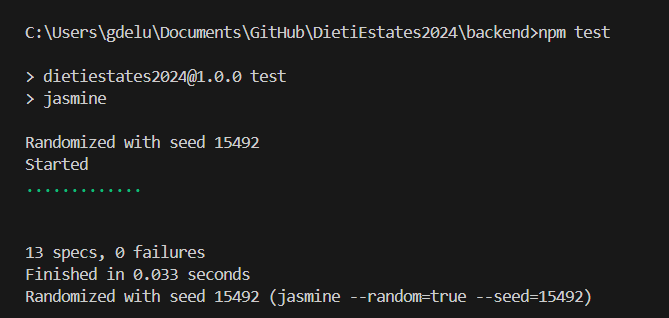
\includegraphics[width=0.7\linewidth]{images/TestResult.png}
    \caption{Esito dell'esecuzione dei 13 Unit Test tramite console (con Jasmine)}
    \label{fig:risultati-console}
\end{figure}
\newpage

\section{Analisi dell'Usabilità e Validazione UI}
Per accertare la qualità dell'interazione uomo-macchina (HCI) all'interno di DietiEstates, è stato strutturato un rigoroso protocollo di validazione. L'obiettivo primario è stato misurare il grado di intuitività del sistema, con un focus mirato sull'efficacia dello storico delle ricerche e sulla tempestività delle notifiche push. La strategia di testing si è divisa in due macro-fasi: una revisione analitica da parte degli addetti ai lavori (Expert Review) e una sessione di validazione sul campo con un campione rappresentativo (Usability Testing).

\subsection{Fase 1: Expert Review e Ispezione Euristica}
Prima di coinvolgere gli utenti, il prototipo è stato sottoposto a una Ispezione Euristica. Il team ha valutato le interfacce utilizzando come perimetro di riferimento le celebri 10 euristiche di Nielsen, declinandole sulle necessità specifiche di un portale immobiliare.

\subsubsection{Definizione della Checklist Sistematica}
Il processo di review è stato guidato dalla seguente checklist valutativa:
\begin{enumerate}
    \item \textbf{Visibilità e Feedback immediato:} Il sistema comunica in tempo reale i cambiamenti? (Verifica focalizzata sul badge delle notifiche push).
    \item \textbf{Aderenza al mondo reale:} I termini utilizzati ("Vani", "Locazione", "Classe Energetica") sono comprensibili senza ambiguità tecniche?
    \item \textbf{Libertà d'azione e reversibilità:} L'utente può facilmente tornare sui propri passi? (Es. visualizzare ricerche precedenti).
    \item \textbf{Standardizzazione visiva:} I bottoni di call-to-action e le gerarchie tipografiche mantengono la stessa coerenza tra la homepage e le viste di dettaglio?
    \item \textbf{Prevenzione strutturale degli errori:} I form di filtraggio bloccano l'inserimento di dati contrastanti (es. prezzo minimo maggiore del massimo)?
    \item \textbf{Supporto cognitivo (Riconoscere vs Ricordare):} L'interfaccia solleva l'utente dallo sforzo mnemonico? \textit{(Punto focale per testare la validità dello "Storico Ricerche")}.
    \item \textbf{Flessibilità d'uso:} Sono presenti shortcut per gli utenti più esperti che desiderano bypassare la navigazione standard?
    \item \textbf{Minimalismo estetico:} Le card degli immobili mettono in risalto la componente fotografica evitando sovraccarichi informativi?
    \item \textbf{Gestione trasparente degli errori:} Le pagine vuote (es. "Nessun immobile trovato") offrono percorsi alternativi chiari?
    \item \textbf{Help contestuale:} La documentazione e i tooltip di supporto sono accessibili direttamente nei punti di maggiore frizione?
\end{enumerate}

\subsubsection{Applicazione della Checklist e Interventi Correttivi}
L'applicazione di questa griglia ha confermato la validità dell'architettura dell'informazione. La feature dello \textit{Storico Ricerche} ha superato a pieni voti il controllo sul "Supporto cognitivo", permettendo di recuperare query complesse con una singola interazione. Allo stesso modo, le \textit{Notifiche} hanno garantito un eccellente livello di "Visibilità e Feedback".
Durante la review sono emerse solo criticità minori: è stato necessario aumentare il contrasto cromatico delle notifiche lette rispetto a quelle da leggere e inserire un pulsante più visibile per il reset totale dei filtri di ricerca.

\subsection{Fase 2: Usability Testing sul Campo}
Risolti i problemi preliminari, si è passati alla conduzione di un test empirico basato sulla metodologia del \textit{Discount Usability Engineering}. L'esperimento ha combinato metriche oggettive (time-on-task) e valutazioni soggettive.

\subsubsection{Procedura Sperimentale, Metriche e Soggetti}
Il campione di test è stato accuratamente profilato per coprire diversi livelli di alfabetizzazione digitale e molteplici casi d'uso (acquisto, affitto, monitoraggio). Le metriche considerate includono il tempo di completamento delle operazioni e il tasso di soddisfazione post-esperimento.

\begin{table}[h!]
    \centering
    \small
    \begin{tabularx}{\textwidth}{c c c c X X}
        \toprule
        \textbf{ID} & \textbf{Età} & \textbf{Genere} & \textbf{Skill IT} & \textbf{Occupazione} & \textbf{Obiettivo del Tester}                                  \\
        \midrule
        P1          & 23           & M               & Avanzata          & Studente Univ.       & Ricerca di immobili economici tramite filtri avanzati e mappa. \\
        P2          & 34           & F               & Media             & Impiegata            & Monitoraggio degli immobili tramite alert e notifiche.         \\
        P3          & 48           & M               & Media             & Professionista       & Utilizzo basato sul recupero dello storico delle ricerche.     \\
        P4          & 58           & F               & Base              & Casalinga            & Navigazione visuale ed esplorazione del portale.               \\
        P5          & 65           & M               & Critica           & Pensionato           & Valutazione della chiarezza delle informazioni.                \\
        \bottomrule
    \end{tabularx}
    \caption{Demografia e profilazione del campione coinvolto nell'esperimento.}
    \label{tab:usability_users}
\end{table}

\subsubsection{Definizione dei Task (Scenari d'Uso)}
Ogni soggetto ha affrontato quattro scenari operativi senza alcun supporto esterno:
\begin{enumerate}
    \item [Task 1] \textbf{Ricerca Strutturata:} Configurare una query inserendo città, range di prezzo e metratura minima.
    \item [Task 2] \textbf{Recupero Rapido:} Interrompere la sessione, tornare alla pagina principale e ripristinare la ricerca precedente usando lo Storico.
    \item [Task 3] \textbf{Gestione Alert:} Notare l'arrivo di un aggiornamento, aprire il pannello notifiche e leggerne il contenuto.
    \item [Task 4] \textbf{Contatto Diretto:} Aprire una scheda immobile e individuare i bottoni per comunicare con l'agenzia di riferimento.
\end{enumerate}

\subsubsection{Survey Post-Esperimento}
Per raccogliere il feedback qualitativo, i tester hanno compilato un questionario basato su scala Likert a 5 punti (1 = Pessimo/Disaccordo, 5 = Ottimo/D'accordo), strutturato per validare i principi di usabilità:

\begin{table}[h!]
    \centering
    \small
    \begin{tabularx}{\textwidth}{c X l}
        \toprule
        \textbf{ID} & \textbf{Domanda di Valutazione}                                     & \textbf{Principio Analizzato} \\
        \midrule
        Q1          & Il vocabolario del portale è stato sempre chiaro e non ambiguo.     & Linguaggio Naturale           \\
        Q2          & Richiamare le mie ricerche passate è stato immediato e utile.       & Carico Cognitivo              \\
        Q3          & Il sistema di notifiche mi ha avvisato in modo tempestivo.          & Visibilità di Stato           \\
        Q4          & L'interfaccia si comporta in modo prevedibile in ogni schermata.    & Coerenza Visiva               \\
        Q5          & Quando ho sbagliato a inserire un filtro, è stato facile rimediare. & Controllo Utente              \\
        Q6          & I messaggi del sistema sono rassicuranti e costruttivi.             & Gestione Errori               \\
        \bottomrule
    \end{tabularx}
    \caption{Questionario di gradimento (Adattamento SUS).}
    \label{tab:usability_survey}
\end{table}

\subsubsection{Analisi e Discussione dei Risultati}
I dati raccolti certificano l'eccellente usabilità del prodotto. Sul fronte dell'efficienza oggettiva (Figura \ref{fig:times}), l'interazione con le Notifiche (Task 3) e lo Storico (Task 2) ha richiesto tempi brevissimi (rispettivamente 12 e 15 secondi di media), dimostrando che le feature abbattono efficacemente i tempi di navigazione. Il Task 1, prevedibilmente più lungo (65 secondi), rientra comunque in un range ottimale per la compilazione di moduli complessi.

\begin{figure}[h!]
    \centering
    \begin{tikzpicture}
        \begin{axis}[
                xbar,
                y axis line style = { opacity = 0 },
                axis x line       = none,
                tickwidth         = 0pt,
                enlarge y limits  = 0.2,
                enlarge x limits  = 0.02,
                symbolic y coords = {Task 4 - Contatto, Task 3 - Alert, Task 2 - Recupero, Task 1 - Ricerca},
                nodes near coords,
                nodes near coords align={horizontal},
                width=10cm,
                height=6cm,
                bar width=15pt,
                fill=blue!30,
                draw=blue!80
            ]
            \addplot coordinates { (45,Task 4 - Contatto) (12,Task 3 - Alert) (15,Task 2 - Recupero) (65,Task 1 - Ricerca) };
        \end{axis}
    \end{tikzpicture}
    \caption{Metriche oggettive: Tempo medio speso per Task (in secondi).}
    \label{fig:times}
\end{figure}

L'analisi soggettiva derivata dal survey (Figura \ref{fig:radar}) conferma pienamente le metriche temporali. La voce Q2 (relativa allo Storico) ha dominato il questionario con un punteggio di 4.8 su 5, confermandosi la funzionalità più apprezzata per l'abbattimento del carico cognitivo. Ottimi risultati anche per le Notifiche (Q3 - 4.6/5). Le uniche lievi flessioni si registrano sulla voce Q5 (4.0/5), suggerendo che, per futuri aggiornamenti, i pulsanti di reset delle form dovrebbero essere resi ancor più evidenti visivamente.



\end{document}